\documentclass[a4paper,12pt]{article}

% -------------------- Paquetes base --------------------
\usepackage[utf8]{inputenc}
\usepackage[T1]{fontenc}
\usepackage[spanish]{babel}
\usepackage{lmodern}
\usepackage{geometry}
  \geometry{margin=2cm}
\usepackage{amsmath,amssymb,physics,dsfont}
\usepackage{graphicx}
\usepackage{multicol}
\usepackage{tikz}
  \usetikzlibrary{positioning,shapes.callouts,shadows,decorations.pathmorphing,shapes.geometric}
\usepackage{pgfplots}
  \pgfplotsset{compat=1.17}
\usepackage{feynmp-auto}
\usepackage{tikz-feynman}

% -------------------- Hiperenlaces y colores --------------------
\usepackage[svgnames]{xcolor}
\usepackage{hyperref}
  \hypersetup{
    colorlinks   = true,
    linkcolor    = DarkBlue,
    urlcolor     = DarkRed,
    citecolor    = DarkGreen,
  }

% -------------------- Microtipografía --------------------
\usepackage{microtype}
\usepackage{ragged2e}
\usepackage{url}

% -------------------- Documento bibliográfico --------------------
\usepackage{natbib}

% -------------------- Títulos secciones --------------------
\usepackage{titlesec}

% -------------------- Carga de estilos personalizados ----

% entornos.tex
% ------------------------------------
% Definición de colores personalizados
\definecolor{DarkBlue}{RGB}{0, 50, 100}
\definecolor{DarkRed}{RGB}{150, 0, 0}
\definecolor{DarkGreen}{RGB}{0, 100, 0}
\definecolor{LightYellow}{RGB}{255, 255, 200}

% Configuración de titlesec
\titleformat{\section}
  {\Large\bfseries\sffamily}
  {\thesection}{1em}{}

\titleformat{\subsection}
  {\large\bfseries\sffamily}
  {\thesubsection}{1em}{}


% Carga de tcolorbox libraries
\usepackage{tcolorbox}
\tcbuselibrary{skins, breakable}

% Ejercicio estándar (azul)
\newtcolorbox{ejercicio}[1][]{
  colback=LightYellow!5,
  colframe=DarkBlue!80!black,
  title=Ejercicio,
  fonttitle=\sffamily\bfseries,
  sharp corners,
  boxrule=0.8pt,
  left=8pt,
  right=8pt,
  top=4pt,
  bottom=4pt,
  enhanced,
  attach boxed title to top left={xshift=5mm, yshift=-2mm},
  boxed title style={colback=DarkBlue!80!black},
  #1
}

% Ejercicio importante (rojo)
\newtcolorbox{ejercicioimportante}[1][]{
  colback=LightYellow!5,
  colframe=DarkRed!80!black,
  title=Ejercicio Importante,
  fonttitle=\sffamily\bfseries,
  sharp corners,
  boxrule=0.8pt,
  left=8pt,
  right=8pt,
  top=4pt,
  bottom=4pt,
  enhanced,
  attach boxed title to top left={xshift=5mm, yshift=-2mm},
  boxed title style={colback=DarkRed!80!black},
  #1
}

% Tarea (verde)
\newtcolorbox{tarea}[1][]{
  colback=LightYellow!5,
  colframe=DarkGreen!80!black,
  title=Tarea,
  fonttitle=\sffamily\bfseries,
  sharp corners,
  boxrule=0.8pt,
  left=8pt,
  right=8pt,
  top=4pt,
  bottom=4pt,
  enhanced,
  attach boxed title to top left={xshift=5mm, yshift=-2mm},
  boxed title style={colback=DarkGreen!80!black},
  #1
}
  %
\usetikzlibrary{positioning,shapes.geometric,decorations.pathmorphing,shadows}
\newtcolorbox{ejercicios}{
  colback=LightYellow!5,
  colframe=DarkBlue,
  title = Ejercicio,
  sharp corners,
  boxrule=0.5pt,
  left=8pt,
  right=8pt,
  top=4pt,
  bottom=4pt,
}


%\titleformat{\section}
%  {\normalfont\LARGE\bfseries}{\thesection}{1em}{}

\begin{document}

\begin{center}
    Julio Fernando Vicente Maldonado\\ 
    \textbf{Altas energías primer semestre 2025 }
\end{center}

\vspace{1cm}
\centerline{\rule{0.95\textwidth}{0.4pt}}
\centerline{\rule{0.95\textwidth}{0.4pt}}

\section{Simetrías y Grupos (representaciones)}

Definición: \\
Es un conjunto de elementos, \( G=\{g_1, g_2, \dots, g_n\} \), que satisface las siguientes propiedades:
\begin{itemize}
    \item \textbf{Cerradura:} Para todo \( g, g' \in G \), se tiene que \( g \circ g' \in G \).
    \item \textbf{Sociativo :} Para todo $g,g' \in G $ , se tiene que  $(g\circ g') \circ g'' = g \circ (g' \circ g'')  $  
    \item \textbf{Identidad:}  Para todo $g \in G$ existe $e \in G$ tal que:  $g \circ e = e\circ g =g$ 
    \item \textbf{Inverso:} para todo $g \in G $ y $g^{-1}\in G $, se tiene $g \circ g^{-1} = g^{-1}\circ g = \mathbb{I} $
\end{itemize}

 

\begin{tikzpicture}[remember picture, overlay]
  \node[rectangle callout, 
        callout relative pointer={(0.6cm, -0.8cm)}, % Ajusta la dirección y longitud de la flecha
        draw, 
        fill=green!10, 
        drop shadow, 
        rounded corners, 
        inner sep=2pt] 
  at (-1,4) {Producto};
  \node[rectangle callout, 
        callout relative pointer={(-1.6cm, -0.4cm)}, % Ajusta la dirección y longitud de la flecha
        draw, 
        fill=green!10, 
        drop shadow, 
        rounded corners, 
        inner sep=2pt] 
  at (15,2.2) {Donde $e$ es la identidad};
\end{tikzpicture}

\subsection{Algunos ejemplos ilustrativos: }
\subsubsection{Grupo $Z_3$ (Permutaciones)} 

\begin{center}
    \begin{table}[h]
    \centering
    \begin{tabular}{c||ccc}
         & $e$& $a$& $b$\\
        \hline \hline
        $e$& $e$& $a$& $b$\\
        $a$& $a$& $b$& $e$\\
        $b$& $b$& $e$& $a$\\
    \end{tabular}
    \label{tab:placeholder_label}
\end{table}
\end{center}
$n $ objetos $(x_1,x_2,\ldots x_n )$ \\
$S_n$ con $n!$ elementos\\
\[  
\begin{array}{cccc}
    n =1  & (x_1) & s_1= \{ e \} & g(x_1)= (x_1)   \\
     n =2  & (x_1,x_2) & s_2= \{ e,g_{12} \} & g_{12}(x_1,x_2)= (x_1)   \\
     n =3  & (x_1,x_2,x_3) & s_3= \{ e,g_{12},g_{23},g_{31},g_{123},g_{132} \} &     \\
     n =3  & (x_2,x_1,x_3) & s_3= \{ e,g_{12},g_{23},g_{31},g_{123},g_{132} \} &     \\
     n =3  & (x_1,x_3,x_2) & s_3= \{ e,g_{12},g_{23},g_{31},g_{123},g_{132} \} &     \\
     n =3  & (x_3,x_2,x_1) & s_3= \{ e,g_{12},g_{23},g_{31},g_{123},g_{132} \} &     \\
     n =3  & (x_3,x_1,x_2) & s_3= \{ e,g_{12},g_{23},g_{31},g_{123},g_{132} \} &     \\
     n =3  & (x_2,x_3,x_1) & s_3= \{ e,g_{12},g_{23},g_{31},g_{123},g_{132} \} &     \\
\end{array}
\]
$S_3$ esta es la única forma de de escribir los elementos. 

\subsection{Grupos  Continuos}
\textbf{Ejemplo:} 
\subsubsection{Grupo unitario de dimensión 1 $U(1)$}

 

\begin{minipage}[t]{0.30\textwidth}
  \centering
  \begin{tikzpicture}
    \begin{axis}[
        axis equal,
        xlabel={$Re(z)$},
        ylabel={$Im(z)$},
        xmin=-1.2, xmax=1.2,
        ymin=-1.2, ymax=1.2,
        axis lines=middle,
        ticks=none,
        clip=false
      ]
      % Círculo unitario
      \addplot [domain=0:360, samples=200, blue, very thick]
      ({cos(x)}, {sin(x)});
      
      % Definir ángulo theta
      \pgfmathsetmacro{\theta}{45}
      
      % Dibujar el radio
      \addplot [red, thick, domain=0:1]
      ({x*cos(\theta)}, {x*sin(\theta)})
      node[pos=1.05, right] {$r,\theta$};
      
      % Marcar el punto en la circunferencia
      \addplot [only marks, mark=*, mark size=2pt, red]
      coordinates {({cos(\theta)}, {sin(\theta)})};
      
      % Arco indicando el ángulo
      \draw [ red] (axis cs:0.3,0) arc (0:\theta:0.3);
      \node [red] at (axis cs:0.4,0.15) {\(\theta\)};
      \draw[dotted] (0,1)--(1,1);
      \node at (1.5,0.5) {$z= x+iy$};
            \node at (1.1,1) {$1$};
    \draw[dotted] (-1 ,0)--(-1,-1);
    \node at (-1.1,-1) {$1$};
    \end{axis}
  \end{tikzpicture}
\end{minipage}
\hfill
\begin{minipage}[t]{0.45\textwidth}
  % Aquí va el texto que acompañará a la figura
  \textbf{$U(1)= \{ \text{exp }(i\theta), \quad 0\leq \theta < 2 \pi \}$ }\\
Esto puede expresarse en un plano complejo, como se ve al lado izquierdo.
\end{minipage}


En el plano carteciano: 
$\mathbb{R} \quad \begin{pmatrix}
    x\\y
\end{pmatrix} $
El grupo especial ortogonal en dos dimensiones, \(\mathrm{SO}(2)\), se define como
\[
\mathrm{SO}(2) = \left\{ R \in \mathbb{R}^{2\times2} \;\middle|\; R^T R = I \quad \text{y} \quad \det R = 1 \right\}.
\]
\begin{tikzpicture}[remember picture, overlay]
  \node[rectangle callout, 
        callout relative pointer={(1.5cm, 0.6cm)}, % Ajusta la dirección y longitud de la flecha
        draw, 
        fill=green!10, 
        drop shadow, 
        rounded corners, 
        inner sep=2pt] 
  at (2,0) {Especial};
  \node[rectangle callout, 
        callout relative pointer={(0.28cm, 0.45cm)}, % Ajusta la dirección y longitud de la flecha
        draw, 
        fill=green!10, 
        drop shadow, 
        rounded corners, 
        inner sep=2pt] 
  at (4,0) {Ortogonal};
  \node[rectangle callout, 
        callout relative pointer={(-1.5cm, 0.5cm)}, % Ajusta la dirección y longitud de la flecha
        draw, 
        fill=green!10, 
        drop shadow, 
        rounded corners, 
        inner sep=2pt] 
  at (7,0) {Matrices $2\times 2$};
\end{tikzpicture}
\vspace{1cm}

Podemos desglosar esta definición de la siguiente forma:

\begin{itemize}
  \item \(\mathbf{S}\) (\emph{Special}): Se refiere a que las matrices tienen determinante \(1\), es decir, preservan la orientación.  
    \[
    \det R = 1.
    \]
  \item \(\mathbf{O}\) (\emph{Orthogonal}): Indica que las matrices son ortogonales, lo que implica que se conserva la norma (o la longitud) y los ángulos. Esto se expresa mediante:
    \[
    R^T R = I,
    \]
    donde \(R^T\) es la traspuesta de \(R\) e \(I\) es la matriz identidad.
  \item El \(2\) en \(\mathrm{SO}(2)\) señala que estamos trabajando con matrices \(2 \times 2\), es decir, en el plano.
\end{itemize}

De esta manera, la definición de \(\mathrm{SO}(2)\) se entiende como el conjunto de todas las matrices \(2 \times 2\) ortogonales con determinante \(1\), que corresponden a las rotaciones en el plano.
\[
\begin{array}{c|c}
     M  \in SO(2) & V^T (\theta )  \\
     M (\theta )v = v(\theta ) & V^T M(\theta )^T M(\theta )V \\
     \text{matriz} & V^T V 
\end{array}
\]

\begin{tcolorbox}[colback=yellow!10, colframe=blue!60!white, title=Ejercicio]
\begin{enumerate}
    \item Mostrar que las matrices \underline{ortogonales } de $2 \times 2$ solo pueden tener $det 1 $o $-1$
    \item  Si el determinante es $(-1)$  corresponde a hacer una rotación y una reflexión. 
\end{enumerate}

\end{tcolorbox}
\fboxrule=3pt

 \fbox
{ 
\begin{minipage}{0.75\textwidth}
\underline{Solución:} \\
$1)$ Recordemos que para que una matriz sea ortogonal debe de cumplirse: 
\[
A \cdot A = A^T \cdot A = \mathbb{I}
\]
Es decir: La inversa de una matriz es su transpuesta:
\[
A^{-1} = A^T
\]
Entonces, podemos extender esto para toda matriz $A $ de tamaño $n \times n $ que sea ortogonal: 
\begin{align*}
det(A \cdot A^T ) &= det (A^T \cdot A )= det (\mathbb{I}) \\
det(A)\cdot det(A^T ) &= det(A^T ) \cdot det (A) =1\\
\Rightarrow det(A)\cdot det(A) &= det(A)\cdot det(A) = 1 \\
det^2(A)  &= 1\\
det(A) &= \pm 1.
\end{align*}
2) Para esto, tomemos el caso de la matriz de rotación pura en $2 \times 2$: 
\[
A=\begin{pmatrix}
\cos \theta &- \sin \theta \\
\sin \theta &\cos\theta
\end{pmatrix}
\]
Primero sabemos que es una matriz ortogonal porqué cumple que: 
\[
A^T \cdot A = \mathbb{I} 
\]
cuyo determinante es 1. 
por otra parte, si tomamos la reflexión pura: 
\[
A= \begin{pmatrix}
    \cos \theta & \sin \theta\\
    \sin \theta & - \cos\theta 
\end{pmatrix}
\]
Para esta matriz ortogonal se tiene en efecto $det A = -1.$

En general podemos decir pues; toda matriz ortogonal \( A \in \text{O}(2) \) con \(\det(A) = -1\) puede expresarse como una \textbf{rotación seguida de una reflexión}. Por ejemplo: \\

Sea \( R \) una reflexión en el eje \( x \):
\[
R = \begin{pmatrix}
1 & 0 \\
0 & -1
\end{pmatrix}, \quad \det(R) = -1.
\]

Una matriz con \(\det = -1\) se escribe como, una rotación seguida de una reflexión:
\[
A = \begin{pmatrix}
\cos\theta & -\sin\theta \\
\sin\theta & \cos\theta
\end{pmatrix} \cdot R = \begin{pmatrix}
\cos\theta & \sin\theta \\
\sin\theta & -\cos\theta
\end{pmatrix}.
\]

\textbf{Esto básicamente es:} \\
  primero hace una \textit{Rotación}: Gira el sistema por \(\theta\). \\  
  luego hace una \textit{Reflexión}: Invierte la coordenada \( y \). \\

Entonces \(\det(A) = -1\) corresponde a una transformación que combina rotación y reflexión.
\end{minipage}
}


\subsection{Transformaciones Infinitesimales}
Para un grupo de Lie \( G \), un elemento \( g(\theta) \) cerca de la identidad (\( \theta = 0 \)) puede expandirse en serie de Taylor como:
\[
g(\theta) = g(0) + \frac{\partial g}{\partial \theta} \bigg|_{\theta=0} \theta + \frac{1}{2} \frac{\partial^2 g}{\partial \theta^2} \bigg|_{\theta=0} \theta^2 + \cdots.
\]
Como \( g(0) = \mathbb{I} \) (la identidad), para \( \theta = \epsilon \ll 1 \), la expansión se reduce a:
\[
g(\epsilon) \approx \mathbb{I} + \frac{\partial g}{\partial \theta} \bigg|_{\theta=0} \epsilon.
\]
El término \( \frac{\partial g}{\partial \theta} \big|_{\theta=0} \) es el \textbf{generador del grupo}, denotado por \( T \). Así, escribimos:
\[
g(\epsilon) = \mathbb{I} + i T \epsilon.
\]

\subsection{Ejemplos de Generadores}
\subsubsection{Grupo \( U(1) \)}
El grupo \( U(1) \) consiste en números complejos de la forma \( g(\theta) = e^{i\theta} \). Su generador se obtiene derivando:
\[
\frac{\partial g}{\partial \theta} \bigg|_{\theta=0} = \frac{\partial}{\partial \theta} e^{i\theta} \bigg|_{\theta=0} = i.
\]
Por lo tanto, el generador de \( U(1) \) es \( T = 1 \).

\subsubsection{Grupo \( SO(2) \)}
El grupo \( SO(2) \) consiste en matrices de rotación en 2D:
\[
M(\theta) = \begin{pmatrix}
\cos\theta & -\sin\theta \\
\sin\theta & \cos\theta
\end{pmatrix}.
\]
Su generador se obtiene derivando:
\[
\frac{\partial M}{\partial \theta} \bigg|_{\theta=0} = \begin{pmatrix}
-\sin\theta & -\cos\theta \\
\cos\theta & -\sin\theta
\end{pmatrix} \bigg|_{\theta=0} = \begin{pmatrix}
0 & -1 \\
1 & 0
\end{pmatrix}.
\]
Por lo tanto, el generador de \( SO(2) \) es:
\[
T = \begin{pmatrix}
0 & -1 \\
1 & 0
\end{pmatrix}.
\]

\subsection{Representaciones de un grupo}
Es un mapeo $D$, de los elementos de $\epsilon $ 
en un set de operadores lineales: 
\begin{align*}
\underbrace{D(\mathbb{I})}_{\mathbb{I}\text{ es la identidad }} &= 1 \tag{1}\\
D(g_1)D(g_2) &= D(g_1\cdot g_2) \tag{2}
\end{align*}
\subsubsection{Ejemplo: Grupo Cíclico de Orden 3}
 Considere el grupo $G = \{e, a, b\}$ que sigue la siguiente regla:
\begin{center}
    \begin{table}[h]
    \centering
    \begin{tabular}{c||ccc}
         & $e$& $a$& $b$\\
        \hline \hline
        $e$& $e$& $a$& $b$\\
        $a$& $a$& $b$& $e$\\
        $b$& $b$& $e$& $a$\\
    \end{tabular}
\caption{Posibles permutaciones ($e = \mathbb{I}$)}
\end{table} 
 
\end{center}
Una \textbf{representación unidimensional} se construye usando raíces cúbicas de la unidad:
\[
\begin{array}{cc}
     D(\mathbb{I }) =1& \overbrace{D(\mathbb{I})}^{1} D(a)  = D(I\cdot a ) = D(a).   \\
     D( a) = e^{\frac{2 }{3} \pi i}&  D(a) D(a) = D(a\cdot a) = D(b).\\
     D(b) = e^{\frac{4}{3}\pi i } & D(a)D(b) = D(a\cdot b) = D(\mathbb{I}).
\end{array}
\]

\subsection{Representación Regular: Construcción}
Para grupos finitos, la \textbf{representación regular} actúa sobre un espacio vectorial con base $\{\ket{g} | g \in G\}$:
 
\begin{enumerate}
    \item Primero construyo una base ortogonal:
\[
\begin{array}{ccc}
     \ket{a} & \ket{b} & \ket{D(\mathbb{I})}
\end{array}
\]
\item  Los elementos de la representación los voy a construir sobre la base: 
\[
D(g_1)  \ket{g_2} = \ket{g_1 \cdot g_2}
\]
\item  Cambiando de notación, los elementos de $D(g)$ van a ser: 
\[
[ D( g) ]_{ij} = \bra{e_i } D(g) \ket{e_j}
\]
\[
\begin{array}{ccc}
    \ket{e_1} = \ket{\mathbb{I}} & \ket{e_2} = \ket{a} & \ket{e_3} = \ket{b}
\end{array}
\]

\end{enumerate}
Entonces tomando: 
\begin{align*}
g&= \mathbb{I} \\
[D(e_1)]_{ij} &= \bra{e_i } D(e_1) \ket{e_j} = \bra{e_i} \ket{\mathbb{ I } e_j} \\
[D(e_1)]_{ij} &=\bra{e_i} \ket{e_j} = \delta_{ij}\\
[D(e_1)]_{ij} &= \begin{pmatrix}
    1&0&0\\
    0&1&0\\
    0&0&1
\end{pmatrix}.
\end{align*}

Para $g= e_2 = a$ 
\[
[D(a) ]_{ij} = \bra{e_i} D(a) \ket{e_j} = \bra{e_i} \ket{a e_j}
\]
tomando los casos correspondientes para: 
\[
\begin{array}{ccc}
     \bra{\mathbb{I}}\ket{a e_j} & \bra{a } \ket{ae_j}     &  \bra{b}\ket{a e_j} 
\end{array}
\]
Se tiene la siguiente matriz: 

\[
[D(a)]_{ij} = \begin{pmatrix}
    0&0&1 \\
    1 &0&0 \\
    0&1&0
\end{pmatrix}
\]





\begin{tcolorbox}[colback=yellow!10, colframe=blue!60!white, title=Ejercicio] 
 
Calcular: $[D(b) ]_{ij} $
\end{tcolorbox}

\fbox
{ 
\begin{minipage}{0.75\textwidth}
\underline{Solución:} 

Hacemos un procedimiento análogo al que se hizo para $e_2=a$;
Para $g= e_3 = b$ 
\[
[D(b) ]_{ij} = \bra{e_i} D(b) \ket{e_j} = \bra{e_i} \ket{b e_j}
\]
tomando los casos correspondientes para: 
\[
\begin{array}{c|c|c}
     \bra{\mathbb{I}}\ket{b e_j} & \bra{a } \ket{be_j}     &  \bra{b}\ket{b e_j} \\
     \bra{\mathbb{I}}\ket{b \mathbb{I}} =0 & \bra{a } \ket{b\mathbb{I} } =0 & \bra{b}\ket{b \mathbb{ I} } =1 \\
     \bra{\mathbb{I}}\ket{b a } =1 & \bra{a } \ket{b a}=0 & \bra{b}\ket{b a } =0  \\
     \bra{\mathbb{I}}\ket{b b} =0 & \bra{a } \ket{b b} =1 & \bra{b}\ket{b b} =0
\end{array}
\]
De esto ya se tiene la siguiente matriz: 
\[
[D(b)]_{ij} = \begin{pmatrix}
0&1&0\\
0&0&1\\
1&0&0
\end{pmatrix}.
\]

\end{minipage}
}

\subsection{Representaciones de grupos continuos}
Para grupos como $SO(2)$ o $SU(2)$, las representaciones se construyen usando \textbf{generadores infinitesimales}. Cerca de la identidad:

Sea $U \in G$ tales que $U(\alpha =0) =1$ (si esto es cierto puedo expandirlos en intervalos pequeños con series de Taylor)
\[
U(\epsilon) = \mathbb{I} + i \epsilon_a T_a + \mathcal{O}(\epsilon^3
) 
\]
Esto es: 
\[
D[\epsilon =0] =1.
\]
La representación más general de $\epsilon$ es
\fbox
{ 
\( 
D(\epsilon ) = \mathbb{I} + i \epsilon_a T_a
\)
}
donde $T_a$ son generadores del álgebra de Lie.

El mapeo del producto de todas las representaciones es: 
\[
D(g_1)D(g_2)\cdots D(g_n)  = D(g_1 \cdot g_2 \cdots g_n)
\]
Si se hace una parametrización exponencial esto es: 
\[
D(\alpha ) = \lim_{k \to \infty } \qty( 1+ i \frac{ \alpha_a}{k}T_a  )^k
\]
\begin{tcolorbox}[colback=yellow!10, colframe=blue!20!black, title=Ejercicio interesante ] 

 Se puede desmostar que exp$[ i \alpha_a T_a]$
\end{tcolorbox}
 
\fbox{ 
\begin{minipage}{0.9\textwidth}
\underline{Solución}

   Para \( k \) grande:
   \[
   \left(\mathbb{I} + \frac{i \alpha_a T_a}{k}\right)^k = \sum_{m=0}^k \binom{k}{m} \left(\frac{i \alpha_a T_a}{k}\right)^m.
   \]
Entonces,    Cuando \( k \to \infty \), tenemos:
   \[
   \binom{k}{m} \frac{1}{k^m} \approx \frac{1}{m!}.
   \]
Por lo tanto:
   \[
   \lim_{k \to \infty} \sum_{m=0}^k \frac{\left(i \alpha_a T_a\right)^m}{m!} = \sum_{m=0}^\infty \frac{\left(i \alpha_a T_a\right)^m}{m!} = \exp\left(i \alpha_a T_a\right).
   \]

\end{minipage}
}


\subsection{Representación exponencial de $SO(2)$}

\[
M(\theta) = \begin{pmatrix}
    \cos \theta &-\sin\theta \\
    \sin\theta & \cos\theta
\end{pmatrix}
\]
El generador $T$ se obtiene derivando en $\theta=0$:
\[
T = - i \frac{\partial M}{ \partial \theta }\big|_{\theta =0 } \quad \Rightarrow T = \begin{pmatrix}
    0 & -1\\
    1 &0 .
\end{pmatrix}
\]
La representación exponencial reconstruye la rotación:
\[
D(\theta) = e^{ i \theta T}
\]
Expandimios esto, y tenemos: 

\begin{align*}
D(\theta  ) &= 1+ i\theta T+ \frac{1}{2} (i\theta T)^2+\ldots + \frac{1}{n!} (i \theta T)^n\\
\text{Tenemos} \\
T^2 &= \begin{pmatrix}
    0 &i\\
    -i&0
\end{pmatrix}\begin{pmatrix}
    0 &i\\
    -i&0
\end{pmatrix} = \begin{pmatrix}
    0 &1\\
    1&0
\end{pmatrix}\\
T^3&= T^2 \cdot T = T 
\end{align*}
Tenemos los siguientes casos: 
\[
 \begin{cases}
     \text{pares} = \mathbb{I} \\
     \text{impares } = T
 \end{cases}
\]

De esto se tiene entonces: 
\[
D(\theta ) = \underbrace{\qty(1+  \sum_{n=1}^\infty \frac{(i\theta )^{2n}}{2n!} )\mathbb{I}}_{\text{pares}} +\underbrace{\sum_{n=0}^\infty\frac{(i\theta)^{ 2n+1} }{(2n+1)! }T  }_{\text{Impares }}
\]

\begin{align*}
D(\theta ) &= \sum_{n=0}^\infty \frac{(i\theta )^{2n}}{(2n)!} \mathbb{I} + \sum_{n=0}^\infty\frac{(i\theta )^{2n+1} }{(2n+1)! } i T\\
D(\theta ) &=\sum_{n=0}^\infty \frac{(-1 )^n \theta^{2n} }{(2n)! } \mathbb{I} + \sum_{n=0}^\infty \frac{(-1)^n \theta^{2n+1}}{(2n+1)!} iT \\
D(\theta ) &=\cos\theta \cdot \mathbb{I} \sin \theta \cdot iT\\
D(\theta ) &=\begin{pmatrix}
    \cos\theta & 0 \\
    0 & \cos\theta 
\end{pmatrix}+ \begin{pmatrix}
    0 & -\sin\theta \\
    \sin\theta &0
\end{pmatrix} \\
D(\theta ) &=\begin{pmatrix}
    \cos\theta & -\sin\theta \\
    \sin\theta & \cos\theta 
\end{pmatrix}.
\end{align*}
Obtenemos de nuevo la matriz de rotación, por lo cual funciona nuestro método aproximado. 

Nosotros vamos a trabajar con los grupos $SU(n)$ y $SO(n)$, 
Estos tienen los siguientes parametros: 
\[
\begin{array}{ccc}
     SO(N)& \text{matrices } n\times n   & \text{restricciones} n \times n  \\
     &\text{como es ortogonal } Det =1 &  1 \\
\end{array}
\]
Dimensión $\frac{1}{2}(N^2-N  )= \frac{N(N-1)}{2} $


\begin{tikzpicture}[remember picture, overlay]
  \node[rectangle callout, 
        callout relative pointer={(-0.75cm, 0.2cm)}, % Ajusta la dirección y longitud de la flecha
        draw, 
        fill=green!10, 
        drop shadow, 
        rounded corners, 
        inner sep=2pt] 
  at (11,1) {No suele quitarnos grados de liverdad};
\end{tikzpicture}
Parámetros para $SU(N) $
\[
\begin{array}{cc}
& \text{Restricciones}\\
\hline
     \text{matrices } n \times n  & 2N^2   \\
     \text{unitaria } U^T\cdot U =1 & N(N-1) \\
     \text{Determinante} & 1\\
     \text{Dimensión} & N^2-1 \quad(eje. SU(2)=3)
\end{array}
\]
\begin{tcolorbox}[colback=yellow!10, colframe=blue!20!black, title=Ejercicio ] 
Para \( U \in SU(2) \), demostrar que cerca de la identidad, \( U(\epsilon) = \mathbb{I} + i \epsilon_a T_a \), donde \( T_a \) son los generadores de SU(2).
\end{tcolorbox}
  
\fbox{
\begin{minipage}{0.9\textwidth}
\textbf{Solución} \\

 El grupo  $SU(2)$  está definido por matrices \( U \) que cumplen:
\[
U^\dagger U = \mathbb{I}, \quad \det(U) = 1.
\]
Cerca de la identidad (\( \epsilon_a \ll 1 \)), una transformación infinitesimal se expande como:
\[
U(\epsilon) \approx \mathbb{I} + i \epsilon_a T_a,
\]
donde \( T_a \) son los  generadores  del grupo. Para $SU(2)$, estos generadores son:
\[
T_a = \frac{\sigma_a}{2}, \quad \sigma_a = \text{Matrices de Pauli},
\]
\[
\sigma_1 = \begin{pmatrix} 0 & 1 \\ 1 & 0 \end{pmatrix}, \quad
\sigma_2 = \begin{pmatrix} 0 & -i \\ i & 0 \end{pmatrix}, \quad
\sigma_3 = \begin{pmatrix} 1 & 0 \\ 0 & -1 \end{pmatrix}.
\]
 

 
Los generadores \( T_a \) cumplen:  

 \textbf{Anticonmutación}:
   \[
   \{T_a, T_b\} = \frac{1}{2} \delta_{ab} \mathbb{I}.
   \] 
   \textbf{Conmutación} (Álgebra de Lie de SU(2)):
   \[
   [T_a, T_b] = i \epsilon_{abc} T_c,
   \]
   donde \( \epsilon_{abc} \) es el símbolo de Levi-Civita.
 
Comparando esto:
 
$SO(2)$: Tiene solo 1 generador (es un grupo abeliano):
  \[
  T = \begin{pmatrix} 0 & -1 \\ 1 & 0 \end{pmatrix}, \quad [T, T] = 0.
  \]
Por otra parte, 
SU(2): Tiene3 generadores no conmutativos, lo que refleja su estructura no abeliana.
 
Para $SU(2)$, cualquier elemento cerca de la identidad puede escribirse como:
\[
U(\epsilon) = \exp\left(i \epsilon_a T_a\right) \approx \mathbb{I} + i \epsilon_a T_a + \mathcal{O}(\epsilon^2).
\]
 Ejemplo:
Si \( \epsilon_1 = \epsilon \), \( \epsilon_2 = \epsilon_3 = 0 \):
\[
U(\epsilon) = \exp\left(i \epsilon T_1\right) \approx \mathbb{I} + i \epsilon \begin{pmatrix} 0 & 1/2 \\ 1/2 & 0 \end{pmatrix}.
\]
\end{minipage}
}

¿Qué características tiene el generador ? 

$U : $  Unitario y cumple $U^\dagger U=1 $
Entonces: 

\begin{align*}
(1- i\epsilon_a T_a^\dagger ) (1+ i\epsilon_a T_a) &= \mathbb{I} \\
1- i\epsilon_a T_a^\dagger+i\epsilon_aT^a +\mathcal{O}(\epsilon^3 )&=1\\
i\epsilon_a T_a^\dagger &= i\epsilon_a T_a\\
T_a^\dagger &= T_a \quad \text{Son matrices Hermíticas !}
\end{align*}

 


 

\begin{tcolorbox}[colback=yellow!10, colframe=red!20!black, title=Ejercicio (Este implica mayor importancia)  ] 
Mostrar que cualquier matriz de $2\times 2$ hemitica y de traza 0 se puede escribir como combinación lineal de las matrices de Pauli.  \[
   X = C_a \sigma_a, \quad \text{donde } \sigma_a = \{\sigma_1, \sigma_2, \sigma_3\}.
   \] 
   
   Los elementos del grupo $SU(2)$ se expresan como:  
   \[
   U = \exp\left(i \alpha_a \sigma_a\right).
   \]


\end{tcolorbox}
\fbox{
\begin{minipage}{0.9\textwidth}
Por definición, \( SU(n) \) es el grupo de matrices unitarias (\( U^\dagger U = \mathbb{I} \)) con determinante 1:  
\[
\boxed{\det(U) = 1}.
\]
En el espacio de matrices \( 2 \times 2 \) hermíticas y traceless tiene dimensión 3. Las matrices de Pauli:  
\[
\sigma_1 = \begin{pmatrix} 0 & 1 \\ 1 & 0 \end{pmatrix}, \quad
\sigma_2 = \begin{pmatrix} 0 & -i \\ i & 0 \end{pmatrix}, \quad
\sigma_3 = \begin{pmatrix} 1 & 0 \\ 0 & -1 \end{pmatrix},
\]  
son hermíticas (\( \sigma_a^\dagger = \sigma_a \)),traceless (\( \text{Tr}(\sigma_a) = 0 \)), y linealmente independientes. Por lo tanto, forman una base para este espacio.

Formalmente esto es: 

Sea \( X \) una matriz \( 2 \times 2 \) hermítica y traceless:  
\[
X = \begin{pmatrix} a & b \\ c & d \end{pmatrix}, \quad X^\dagger = X \implies a, d \in \mathbb{R}, \quad c = b^*.
\]  
Además, \( \text{Tr}(X) = a + d = 0 \implies d = -a \).  
Expresando \( X \) en términos de \( \sigma_a \):  
\[
X = C_1 \sigma_1 + C_2 \sigma_2 + C_3 \sigma_3 = \begin{pmatrix} C_3 & C_1 - i C_2 \\ C_1 + i C_2 & -C_3 \end{pmatrix}.
\]  
Igualando componentes:  
\[
C_3 = a, \quad C_1 = \text{Re}(b), \quad C_2 = \text{Im}(b).
\]  
Por lo tanto, toda matriz \( X \) admite una descomposición en términos de \( \sigma_a \).

Por otra parte: 
Las matrices \( i \sigma_a \) son generadores del álgebra de Lie \( \mathfrak{su}(2) \), que consiste en matrices antihermíticas (\( X^\dagger = -X \)) y traceless.  

Por el  teorema de exponenciación de Lie , la aplicación exponencial lleva el álgebra de Lie al grupo:  
   \[
   \exp: \mathfrak{su}(2) \to SU(2).
   \]  
Para \( \alpha_a \in \mathbb{R} \), \( i \alpha_a \sigma_a \) es antihermítica y traceless, por lo que \[(   U= \exp(i \alpha_a \sigma_a) \in SU(2) \]


\end{minipage}
}
\subsection{Álgebras de Lie}

Consideremos un elemento de la representación: 
\[
u(\lambda) = \text{exp} [i \lambda \epsilon_a T_a]
\]
Aplicando la regla de multiplicación del grupo
\[
u(\lambda_1) u(\lambda_2) = u(\lambda_1+\lambda2)
\]
Sin embargo, si los elementos son generados por una combinación lineal diferente
\[
e^{i \alpha_aT_a} e^{i \beta_aT_a} \not= e^{i (\alpha_a 
 + \beta_a)T_a}
\]
Los elementos de la representación deben de poder expresarse como el  exponente de una combinación lineal de los generadores. 
\[
e^{i \alpha_aT_a} e^{i \alpha_aT_a} = e^{i \delta_aT_a} \quad \text{para algún } \delta
\]
Podemos construir una representación utilizando la parametrización exponencial. Para $T_a$ los generadores de $G$ $D(\alpha) = e^{i \alpha_aT_a}$ es una representación de $G$ por lo que tendrá que ser cierto que: 
\[
e^{i \alpha_aT_a} e^{i \beta_bT_b} = e^{i \delta_cT_c}\quad \text{ donde } \delta_a \not = \alpha_a+\beta_a
\]
Consideremos una transformación infinitesimal
\[
i \delta_cT_c = \ln (e^{i \alpha_aT_a} e^{i \beta_bT_b} + \mathbb{I} - \mathbb{I}  )
\]
Intentemos escribir esta expresión como $\ln ( \mathbb{I} + l)$, si $k$ es infinitesimal podemos expandir alrededor de $k=0$. 

Para una transformación infinitesimal $\alpha_a, \beta_a$ son pequeños 
\[
k = e^{i \alpha_aT_a} e^{i \beta_bT_b}  - \mathbb{I}
\]
Expandiendo hata segundo orden tenemos: 
\begin{align*}
    k &= [1+ i \alpha_a T_a -1/2 (\alpha_aT_a)^2] [1+i\beta_bT_b -1/2 (\beta_bT_b)^2] -1\\
    &= 1+ i \alpha_aT_a+i\beta_bT_b -\alpha_a T_a \beta_bT_b -\frac{1}{2} ( \alpha_aT_a)^2 -\frac{1}{2} (\beta_bT_b)^2-1 
\end{align*}
Para $k $ pequeño se tiene: 
\begin{align*}
    i \delta_cT_c &= \ln(1+k )  = k-\frac{1}{2}k^2+\dots\\
    &= i \alpha_aT_a +i\beta_bT_b -\alpha_aT_a\beta_bT_b-\not\frac{1}{2} (\alpha_a T_a)^2-\not\frac{1}{2}(\beta_bT_b)^2    \\
    &\underbrace{-\frac{1}{2} (i \alpha_aT_a + i\beta_bT_b })^2+\dots\\
    & \frac{1}{2 }(\alpha_aT_a)^2+ \frac{1}{2}(\beta_bT_b)^2+\frac{1}{2} \alpha_aT_a\beta_bT_b + \frac{1}{2}    \beta_bT_b \alpha_aT_a\\
    i\delta_cT_c&= i \alpha_aT_a + i\beta_bT_b   - \frac{1}{2-} \alpha_a\beta_b (T_aT_b-T_bT_a)+ \dots \\
    &= i\alpha_aT_a + i \beta_bT_b-\frac{1}{2} \alpha_a\beta_b [T_a,T_b]
\end{align*}
El conmutador del álgebra juega un papel similar al producto del grupo:
\[
[T_a, T_b ] = i \underbrace{f_ {abc}} T_c
\]
Donde $f_{abc}$ Se le conoce como constante de estructura del grupo. 
\[
\to \delta _c = ( \delta_{ac}\alpha_a +\delta_{bc}\beta_b  +f_{abc}\alpha_a \beta_b  ) 
\]
\fbox{Ejemplo } Las rotaciones en $3D $ están descritas por los elementos de $SO(3)$ 
\[
R(\theta, \phi, \psi )= \begin{pmatrix}
    1&0&0\\0&\cos\theta & -\sin\theta \\0 &\sin\theta & \cos\theta
\end{pmatrix} \begin{pmatrix}
    \cos\phi&0& \sin\phi \\ 0&1&0\\-\sin\phi &0&\cos\phi 
\end{pmatrix} \begin{pmatrix}
    \cos\psi & - \sin\psi &0\\ \sin\psi &\cos\psi &0 \\0&0&1
\end{pmatrix}
\]
Necesitamos 3 parámetros para describir un elemento de $SO(3) \to$
3 generadores. 
Estos generadores son: 
\[
J_1 = i \frac{\partial R}{\partial\theta}\big|_{\theta,\phi, \psi =0} = i\begin{pmatrix}
    0&0&0\\0&0&-1\\0&1&0
\end{pmatrix}, \quad J_2 = i \frac{\partial R}{\partial\phi}\big|_{\theta,\phi, \psi =0} = i\begin{pmatrix}
    0&0&1\\0&0&0\\-1&0&0
\end{pmatrix} 
\]
\[
J_3 = i \frac{\partial R}{\partial\psi}\big|_{\theta,\phi, \psi =0} = i\begin{pmatrix}
    0&-1&0\\1&0&0\\0&0&0
\end{pmatrix}
\]
Donde 
\[ 
D(\theta_a)  = \text{exp}[-i \theta_a J_a ]
\]
\[
\theta_a= \theta_1,\theta_2,\theta_3 = \theta, \phi, \psi 
\]
\[
J_a = i \frac{\partial R}{\partial\theta_a }\big|_{\theta_a =0}
\]

\begin{tcolorbox}[colback=yellow!10, colframe=red!20!blue, title=Ejercicio  ] 
 Mostrar que el álgebra de Lie de $SO(3) $ 
\[
[J_a,J_b ] = i \epsilon_{abc} J_c
\]

\end{tcolorbox}
\fbox{
\begin{minipage}{0.9\textwidth}
\underline{Solución}
Queremos demostar que  los generadores de $SO(3)$ satsfacen la relación de conmutación. 

Entonces, cambiando de notación a los generadores por comodidad a $L_a$, que serían: 
\[
J_a = i L_a
\]


Entonces, probemos pues los valores para las diferentes combinaciones, tomemos: 
\[[J_1,J_2] \]
Usando el combenio definido anteriormente tenemos: 
\begin{align*}
    [J_1,J2 ] &= J_1J_2 -J_2J_1 \\ &= (i L_1) (iL_2) -(iL_2)(iL_1 )\\
    J_1J_2 &= i^2L_1L_2 = -L_1L_2 \\
    J_2J_1 &= -L_2L_1\\
    [J_1,J_2] &= -( L_1L_2-L_2L_1) = -[L_1,L_2]
\end{align*}
Pero ya sabemos que \[[L_1L_2] = \epsilon_{123}L_3  \]
Como $\epsilon_{123} =1$, tenemos que: 
\[
[J_1,J_2] = -L_3
\]
Si tomamos $J_3 = i L_3$, tnemos que 
\[
L_3 = \frac{J_3}{ i} = -i J_3
\]
Entonces:
\[
[J_1,J_2] = -(-iJ_3) = i J_3
\]

 Esto podemos verlo con el  cálculo explícito de \([J_1, J_2]\) 
Primero haciendo el Productos matriciales:
\[
J_1 J_2 = \begin{pmatrix} 0 & 0 & 0 \\ 1 & 0 & 0 \\ 0 & 0 & 0 \end{pmatrix}, \quad
J_2 J_1 = \begin{pmatrix} 0 & 1 & 0 \\ 0 & 0 & 0 \\ 0 & 0 & 0 \end{pmatrix}.
\]

Tenemos el conmutador:
\[
[J_1, J_2] = J_1 J_2 - J_2 J_1 = \begin{pmatrix} 0 & -1 & 0 \\ 1 & 0 & 0 \\ 0 & 0 & 0 \end{pmatrix}.
\]

Notemos que este es el generador $J_3$
\[
[J_1, J_2] = i J_3, \quad \text{donde } J_3 = i \begin{pmatrix} 0 & -1 & 0 \\ 1 & 0 & 0 \\ 0 & 0 & 0 \end{pmatrix}.
\]

\subsubsection*{Generalización }
El símbolo de Levi-Civita \( \epsilon_{abc} \) captura todas las combinaciones:
\[
[J_a, J_b] = i \epsilon_{abc} J_c.
\]
Por ejemplo:
\[
[J_2, J_3] = i J_1, \quad [J_3, J_1] = i J_2.
\]

\end{minipage}
}

¿Qué nos dice el álgebra de Lie sobre cómo se comportan las rotaciones? 

Consideremos una rotación infinitesimal ($\epsilon$) alrededor de $x$, luego $\eta $  al rededor de $y $ luego $-\epsilon$ alrededor d e $x$ y luego $- \eta $ alrededor de $y$ 
\[
R_y(-\eta)R_x(- \epsilon ) R_y (\eta) R_x(\epsilon)
\]
Esto es 
\begin{align*}
    & \qty(\mathbb{I}-i \eta J_2 -\frac{1}{2} \eta^2J_2^2 ) \qty(1+i \epsilon J_1 -\frac{1}{2}\epsilon^2J_1^2  )R_y(\eta) R_x (\epsilon )\\
    &= (1+ i \eta J_2+ i \epsilon J_1- \eta \epsilon J_2J_1-\frac{1}{2} \eta^2 J^2- \frac{1}{2} \epsilon^2J_1^2   )\\
    &\times   (1- i \eta J_2- i \epsilon J_1- \eta \epsilon J_2J_1-\frac{1}{2} \eta^2 J^2- \frac{1}{2} \epsilon^2J_1^2   )\\
    &= 1+i \eta J_2+i \epsilon J_1 -i J_2-i\epsilon J_1\\
    & \eta^2 J_2^2 +\eta\epsilon J_2J_1 +\eta \epsilon J_1 J_2 +\epsilon ² J_1 ^2\\
    & - \eta \epsilon J_2 J_1  - \frac{1}{2} \eta^2 J_2^2- \frac{1}{2} \epsilon^2J^2_1 - \eta \epsilon J_2 J_1 - \frac{1}{2} \eta^2 J_2^2 -\frac{1}{2} \epsilon^2 J_1^2\\
    &= 1 + \eta \epsilon (J_1J_2 -J_2J_1 ) = 1 + \eta \epsilon [J_1, J_2] \\
    &= 1 + \eta \epsilon (-i)  \epsilon_{123}J_3 = 1- i (\eta \epsilon ) J_3 \\
    \to &= \text{ exp }( -i \eta \epsilon J_3) 
\end{align*}
Esto equivale a una rotación en $\epsilon \eta$ alrededor del eje $z$  
\subsection{ La identidad de Jacobi}
Los generadores satisfacen la identidad: 
\[
[T_a, [T_b,T_c] ]+[T_b, [T_c,T_a] ] +[T_c, [T_a,T_b] ] =0
\]
\begin{tcolorbox}[colback=yellow!10, colframe=red!20!blue, title=Ejercicio] 
 Mostrar que los generadores de las álgebras de Lie ( para representaciones de dimensió finita) cumplen con la identidad de Jacobi

\end{tcolorbox}
\fbox{
\begin{minipage}{0.9\textwidth}
\underline{Solución}


Calculemos cada término de la identidad de Jacobi usando la definición del conmutador.

Entonces, para el primer Término:

\[
\begin{aligned}
[T_a, [T_b, T_c]] &= T_a[T_b, T_c] - [T_b, T_c]\,T_a \\
&= T_a(T_b T_c - T_c T_b) - (T_b T_c - T_c T_b)T_a \\
&= T_aT_bT_c - T_aT_cT_b - T_bT_cT_a + T_cT_bT_a.
\end{aligned}
\]

Para el segundo Término: 

\[
\begin{aligned}
[T_b, [T_c, T_a]] &= T_b[T_c, T_a] - [T_c, T_a]\,T_b \\
&= T_b(T_c T_a - T_a T_c) - (T_c T_a - T_a T_c)T_b \\
&= T_bT_cT_a - T_bT_aT_c - T_cT_aT_b + T_aT_cT_b.
\end{aligned}
\]

y para el tercer término:

\[
\begin{aligned}
[T_c, [T_a, T_b]] &= T_c[T_a, T_b] - [T_a, T_b]\,T_c \\
&= T_c(T_a T_b - T_b T_a) - (T_a T_b - T_b T_a)T_c \\
&= T_cT_aT_b - T_cT_bT_a - T_aT_bT_c + T_bT_aT_c.
\end{aligned}
\]

 

Sumando las expresiones anteriores, obtenemos:

\[
\begin{aligned}
&\quad\, \Bigl(T_aT_bT_c - T_aT_cT_b - T_bT_cT_a + T_cT_bT_a\Bigr) \\
&+ \Bigl(T_bT_cT_a - T_bT_aT_c - T_cT_aT_b + T_aT_cT_b\Bigr) \\
&+ \Bigl(T_cT_aT_b - T_cT_bT_a - T_aT_bT_c + T_bT_aT_c\Bigr).
\end{aligned}
\]

Ahora agrupamos los términos:

Notemos que los términos \(T_aT_bT_c\) aparecen en el primer y tercer grupo con signos \(+1\) y \(-1\) respectivamente:
  \[
  T_aT_bT_c - T_aT_bT_c = 0.
  \]
Y que los términos \(T_aT_cT_b\) aparecen con \(-1\) en el primer grupo y \(+1\) en el segundo grupo:
  \[
  -T_aT_cT_b + T_aT_cT_b = 0.
  \]
Además los términos \(T_bT_cT_a\) aparecen con \(-1\) en el primer grupo y \(+1\) en el segundo grupo:
  \[
  -T_bT_cT_a + T_bT_cT_a = 0.
  \]
Finalmente los términos \(T_cT_bT_a\) aparecen con \(+1\) en el primer grupo y \(-1\) en el tercer grupo:
  \[
  T_cT_bT_a - T_cT_bT_a = 0.
  \]
Y de la misma forma, los otros términos (\(T_bT_aT_c\), \(T_cT_aT_b\)) se cancelan de forma similar.

Cada término se cancela exactamente con otro, lo que nos lleva a

\[
[T_a, [T_b, T_c]] + [T_b, [T_c, T_a]] + [T_c, [T_a, T_b]] = 0.
\]

 \end{minipage}
}
 \subsection{ La representación adjunta}
Consideremos el álgebra de Lie $[T_a, T_b ] = if_{abc} T_c $ 
Tomando 
\[
[T_a, [T_b,T_c ]] = i f_{bcd } [T_a, T_d] = -f_{bcd }f_{ade} T_e
\]
La identidad de Jacobi toma la forma: 
\[
f_{bcd }f_{ade} +f_{cad }f_{bde}+ f_{abd}f_{cde}=0
\]
Si definimos 
\[
[Y_a ]_{bc } = - i f_{abc} 
\]
para $f_{acb} = \epsilon_{abc}$ 
\[
[Y_1 ]_{ab} = - i \epsilon_{1bc} = - i \begin{pmatrix}
    0&0&0\\0&0&1\\0&-1&0
\end{pmatrix}
\]
Reescribiendo la identidad de Jacobi 
\begin{align*}
    -f_{cb\textbf{d}} f_{a\textbf{d} e} + f_{ab \textbf{d} }f_{c\textbf{d}e }&= f_{cad } f_{dbe}\\
    (-i f_{cbd}) (- if_{ade} )-(-i f_{abd})(- i f_{cde})  &= if_{cad} [Y_d]_{be} \\
    Y_cY_a -Y_aY_c &= i f_{cad } Y_{d} \quad | \quad \text{para  } f_{abc } = \epsilon_{abc} \\
    [Y_a,Y_c] &= i f_{acd }Y_c \quad | \quad Y_a 
\end{align*}
$Y_a$ son los generadores de $SO(3)$
\textit{Los generadores de  $SO(3)$ son los generadores de la representación adjunta de SU (2)  } 

\subsection{ Estados y operadores }
Los elementos de una representación $\to$ Operadores lineales
\[
x_a \ket{i } = \sum_j \ket{j} \bra{j} x_a\ket{i} = \sum_{\delta} \ket{j} [x_a]_{ij}
\]
El elemento del grupo $e^{i\alpha_a T_a}$ transforma un ket
\[
\ket{i  } \to \ket{i ' } = e^{i \alpha_a T_a } \ket{i}
\]
y para un bra 
\[
\bra{i } \to \bra{i '} = \bra{i } e^{ i \alpha_a T_a}
\]
Al aplicar un operador $\mathcal{O}$ 
\[
\mathcal{O }\ket{ i } \to e^{i \alpha _a T_a } (\mathcal{ O} \ket{i})
\]
\[
\underbrace{e^{i \alpha_a T_a } \mathcal{O }e^{ -i \alpha_a }T_a}_{\mathcal{O'}}   \underbrace{ e^{i \alpha_a }T_a \ket{i } }_{\ket{i'}} 
\]
Los operadores transforman 
\[
\mathcal{O} \to \mathcal{O' } = e^{i \alpha_a T_a } \mathcal{O} e^{-i \alpha_a T_a }
\]
Para una transformación infinitesimal 
\begin{align*}
    e^{i \alpha_a T_a } &\to 1 +\delta \\
    - i \delta \ket{i } &= -i [(1+i \alpha_a T_a )\ket{i }- \ket{i}   ] = \alpha_aT_a \ket{i }\\ 
    \bra{i } i \delta &= \bra{i } \alpha_aT_a \\
    \text{Para el operador }  \mathcal{O}
\end{align*}
\begin{align*}
    - i [ (1+ i \alpha_aT_a)\mathcal{O} (1-i\alpha_aT_a)- \mathcal{O }  ] &= -i \delta \mathcal{O} \\
    - i [\mathcal{O }+i\alpha_aT_a \mathcal{O}- \mathcal{O } i\alpha_aT_a  ]-\mathcal{O}   &= -i \delta \mathcal{O } \\
    -i \delta\mathcal{ O } &= [\alpha_aT_a, \mathcal{O} ].
\end{align*}
La invarianza de la matriz de elementos $\bra{i }\mathcal{ O } \ket{i} $ 
\[
\bra{i } \mathcal{O } (T_a\ket{i }) + \bra{i } [T_a, \mathcal{ O}] \ket{i } - (\bra{i } x_a) \mathcal{O} \ket{i}=0.
\]

\subsection{ Momento Angular}
Un espacio de $N $  dimensiones. asumimos que este espacio transforma bajo una representación de $SU(2)$
\begin{itemize}
    \item Que nos dice el álgebra sobre esta representación 
    \item Diagonalizar tantos elementos como sea posible
\end{itemize}

Álgebra de Lie de $SO(3) $ 
\[
[J_i, J_j] = i \epsilon_{ijk} J_k
\]


$SU(2) :$ Solo podemos diagonalizar un  generador. $J_3$ 

El estado con el elemento más grande es $j $   
\[
J_3 \ket{m} = m \ket{m } \quad m< j
\]
Si definimos los operadores $J^+$ y $J^-$ como 
\[
J^\pm = (J_1 \pm iJ_2)/ \sqrt{2}
\]
\begin{align*}
    [J_3,J^\pm] &= \pm J^\pm \\
    [J^+, J^-] &= J_z
\end{align*}
Se puede mostrar que si el espacio es finito $-j < -m $
\[  
 \text{Ejercicio, ver Georgi} \begin{cases}
    \bra{j, m' } J_3 \ket{j,m } = m \delta_{mm'}  \\
    \bra{j, m' } J^+ \ket{j, m} = \sqrt{ (j+m+1)(j-m )/2  }\delta_{m', m+1 }\\
    \bra{j, m' } J^-\ket{ j, m} = \sqrt{ (j+m)(j-m+1) /2 }\delta_{m', m-1  }
\end{cases}
\]

Los elementos de matriz para la representación espín $j$
\begin{align*}
    [J^j_a]_{kl } &= \bra{j, j+1-k } J_a \ket{j, j+1-l } \quad k, l = \to 2j+1 \text{ posiciones} \\
    [J_a^j]_{mm'} &= \bra{j, m' } J_a \ket{j,m } \quad m,m' \to -j, j
\end{align*}
Para $J = 1/2 $ 
\begin{align*}
        [J_+ ^{1/2}]_{m', m}  &= \sqrt{(j+m +1 ) (j-m)/2 }  \delta_{m', m+1} \quad J_+^{1/2} = \begin{pmatrix}
            0&1\\0&0 
        \end{pmatrix} \frac{1}{\sqrt{2} } \\
        m &= -\frac{1}{2} \to  \sqrt{ \qty(\frac{1}{2}-\frac{1}{2} +1   ) \qty(\frac{1}{2} +\frac{1}{2}  )/2-   } = \frac{1}{\sqrt{2}}
\end{align*}
\begin{align*}
    [J_+^{1/2} ]_{m',m} &= \sqrt{(j+m  ) (j-m+1)/2 }  \delta_{m', m-1} \quad J_-^{1/2} = \begin{pmatrix}
            0&0\\1&0 
        \end{pmatrix} \frac{1}{\sqrt{2} } \\
\end{align*}
\begin{align*}
    J_1 &= \frac{\sqrt{2}}{2} \qty(J_+ +J_-   ) = \frac{1}{2} \begin{pmatrix}
        0&1\\1&0
    \end{pmatrix} \\
    J_2 &= - i \frac{\sqrt{2}}{2 } \qty(J_+-J_- ) = \frac{1}{2}\begin{pmatrix}
        0&-i\\i&0
    \end{pmatrix} \\
    J_3 &= \begin{pmatrix}
        \frac{1}{2} &0 \\ 0 &- \frac{1}{2}
    \end{pmatrix}
 \end{align*}

\begin{tcolorbox}[colback=yellow!10, colframe=red!20!black, title=Ejercicio(como vendría en el examen ) ] 
Obtener los generadores de la representación para $j=1, j = \frac{3}{2}$ 
\end{tcolorbox}
\fbox{
\begin{minipage}{0.9\textwidth}
\underline{Solución}

Asumimos que se cumple el álebra: 
\[
[J_i,J_j] = i \epsilon_{ijk} J_k
\]
Además de que los operadores escalera son: 
\[
J^\pm = \frac{1}{ \sqrt{2}} (J_1 \pm i J_2) 
\]
Entonces, nuestra base de estados $\{ \ket{j,m} \}$ es; 
\[
J_3 = \ket{j, m } = m \ket{j, m } 
\]

\begin{align*}
    J_+ \ket{j,m } &= \sqrt{(j-m)(j+m +1) } \ket{j, m+1} \\
    J_- \ket{j,m } &= \sqrt{(j+m)(j-m +1) } \ket{j, m-1}
\end{align*}
Entonces, las representaciónes para $j =1 $

Definimos los estados de la base como:
\[
\ket{1,1}, \quad \ket{1,0}, \quad \ket{1,-1}
\]

Y recordando que: 
\[
J_3 =  \ket{1,m} =m \ket{1,m}, \quad m=0,1,-1
\]
\[
J_3 = \begin{pmatrix}
    1&0&0\\
    0&0&0\\
    0&0&-1
\end{pmatrix}
\]
Entonces tomando 
\begin{align*}
    J_+ \ket{1, m} &= \sqrt{(1-m)(1+m+1) } \ket{1,m+1} \\
    J_- \ket{1, m} &= \sqrt{(1+m)(1-m+1) } \ket{1,m-1} 
\end{align*}
Entonces, tenemos:
\begin{align*}
    J_+ \ket{1,1}&=0  \\
    J_- \ket{1,1} &= \sqrt{(1+1)(1-1+1) } \ket{1,0} = \sqrt{2} \ket{1,0}\\
    J_+\ket{1,0} &= \sqrt{(1-0) (1+0+1)} \ket{1,1} = \sqrt{2} \ket{1,1} \\
    J_- \ket{1,0} &= \sqrt{(1,0)(1-0+1) } \ket{1,-1} =\sqrt{2} \ket{1,-1} \\
    J_-\ket{1,-1}&= 0 \\
    J_+ \ket{1,-1} &= \sqrt{(1-(-1) )(1+(-1)+1)  }\ket{1,0} = \sqrt{2 } \ket{1,0}
\end{align*}
\[J_+ =
\begin{pmatrix}
    0&\sqrt{2} &0\\ 0&0&\sqrt{2} \\0&0&0
\end{pmatrix}
\]

\end{minipage}
}

\fbox{
\begin{minipage}{0.9\textwidth}
y para $J_- $ 

\[
J_- = J_+^\dagger = \begin{pmatrix}
    0&0&0\\
    \sqrt{2} &0&0 \\
    0&\sqrt{2}&0
\end{pmatrix}
\]
Entonces, los generadores son: 
\begin{align*}
    J_1&= \frac{1}{\sqrt{2} } (J_+ +J_-) \\
    J_1 &= \frac{1}{\sqrt{2} } \begin{pmatrix}
        0& \sqrt{2} &0 \\ \sqrt{2} &0&\sqrt{2} \\0& \sqrt{2} &0
    \end{pmatrix} = \begin{pmatrix}
        0&1&0\\1&0&1\\0&1&0
    \end{pmatrix} \\
    J_2&= \frac{1}{i \sqrt{2}} ( J_+-J_-) \\
    J_2 &= \frac{1}{i \sqrt{2}}\begin{pmatrix}
        0&\sqrt{2} &0 \\ -\sqrt{2} &0&\sqrt{2} \\
        0&- \sqrt{2} &0 
    \end{pmatrix} = \begin{pmatrix}
        0&-i&0\\i&0&-i \\0&i&0
    \end{pmatrix}
\end{align*}

Para $j =3/2$ tenemos 
\end{minipage}

}

\subsection{$SU(2)$ de isospín}

Los  nucleones pueden ser vistos como si fueran 2 grados de libertad.  (Protón \hspace{1cm} neutrón )

$SU(2)$ transforma $(n,p )$ 

\[
p = \begin{pmatrix}    1\\0\end{pmatrix}  \quad n =\begin{pmatrix}    0\\1\end{pmatrix}
\]
\begin{center}
    \begin{tikzpicture}
    \draw[dashed] (0,0) -- (4,0); 
    \node[above] at (1,0.05) {$ n$};
    \node[above] at (3,0.05) {$ p$};
    \fill (1,0) circle (2pt);
    \fill (3,0) circle (2pt);
    \draw[arrows=->] (1,0.6) -- (3,0.6);
    \draw[arrows=->] (3,-0.6) -- (1,-0.6);
    \node[] at (2,1){$\frac{1}{2}(T_1 \pm i T_3) $ };
    \node[] at (4.1,0){$T_3$};
    \end{tikzpicture}
\end{center}

\subsection{El grupo $SU(3) $ y la carga de color. } 


 ¿Cuántos grados de libertad? 
 \[
 n^2 -1 = 8 \quad \text{grados de libertad}
 \]

Es posible tener 2 matrices diagonales. 

Una base de la representación fundamental de $SU(3) $ 
\[
R=\begin{pmatrix} 1\\0\\0 \end{pmatrix}\quad G = \begin{pmatrix}0\\1\\0\end{pmatrix} \quad B = \begin{pmatrix}0\\0\\1\end{pmatrix}
\]

\begin{center}
    \begin{tikzpicture}
    \draw[ ] (-2,0) -- (2,0);
    \draw[ ] ( 0,-2) -- (0,2);
    \node[above] at (-1,1.1) {$ G$};
    \node[above] at (1,1.1) {$ R$};
    \node[above] at (-0.1,-1) {$ B$};
    \fill (-1,1) circle (2pt);
    \fill (1,1) circle (2pt);
    \fill (0,-1) circle (2pt);
    \draw[arrows=->] (-0.8,1) -- (0.8,1);
    \draw[arrows=->] (0.8,0.8) -- (-0.8,0.8);
    \draw[arrows=->] (-1.5,1) -- (-0.5,-0.8);
    \draw[arrows=->] (-0.3,-0.7) -- (-1.2,0.8);
    \draw[arrows=->] ( 0.2,-0.8) -- (1.2, 0.8);
    \draw[arrows=->] (1.5,0.8) -- (0.5,-0.8);
    \node[] at (0,2){$\frac{1}{2}(\lambda_1 \pm i \lambda_2) $ };
    \node[] at (-1.9,-0.4){$\frac{1}{2}(\lambda_6 \pm i \lambda_7) $ };
    \node[] at (1.9,-0.5){$\frac{1}{2}(\lambda_4 \pm i \lambda_5) $ };
    \end{tikzpicture}
\end{center}

\begin{align*}
    \qty[\frac{\lambda_i}{2 ,}, \frac{\lambda_j}{2} ] &= i \sum_k f_{ijk} \frac{\lambda_k }{2}
\end{align*}
$f_{ijk}$ es anti simétrico. 
\[
f_{123} =1  \quad f=_{458} = f_{678} = \frac{\sqrt{3}}{2}
\]
\[
f_{147} =f_{165} =f_{246} = f_{257} = f_{376} = \frac{1}{2}
\]








\subsection*{Transformaciones de Lorentz}
Tomando: 
\begin{align*}
    x' &= \frac{x -vt}{\sqrt{1-\frac{u^2}{c^2}} } \quad t' = \frac{t-\frac{ux}{c^2}}{\sqrt{1-\frac{u^2}{c^2}} } \\
    \begin{pmatrix}
        ct'\\x'\end{pmatrix} &= \begin{pmatrix}
            \gamma & - \beta \gamma \\ - \beta\gamma & \gamma \end{pmatrix} \begin{pmatrix}
                ct\\x
            \end{pmatrix}
\end{align*}
donde $\beta= \frac{u}{c}$ y$ \gamma = \frac{1}{\sqrt{1-\frac{u^2}{c^2 }} } $ 
\[
c^2t^2- x^2 = cte
\]
Ahora, $\beta = \tanh\theta$
\begin{align*}
\gamma &= \frac{1}{\sqrt{1-\beta^2}   } = \frac{1}{\sqrt{1-\tanh^2\theta }} = \frac{\cosh \theta}{\sqrt{\cosh²\theta -\sinh^2\theta} } = \cosh\theta \\
\begin{pmatrix}ct' \\x'\end{pmatrix} &= \begin{pmatrix}
    \cosh \theta &-\sinh \theta \\ - \sinh\theta & \cosh\theta 
\end{pmatrix} \begin{pmatrix}
    ct \\x
\end{pmatrix} \\
\text{Multiplicando por} \\
\times \begin{pmatrix}    i&0\\0&1\end{pmatrix} & \\
    \begin{pmatrix} ict' \\x'\end{pmatrix} &= \begin{pmatrix}
    i&0\\0&1\end{pmatrix}\begin{pmatrix}
    \cosh \theta &-\sinh \theta \\ - \sinh\theta & \cosh\theta 
\end{pmatrix}\begin{pmatrix}
    -i&0\\0&1\end{pmatrix} \begin{pmatrix}
    i&0\\0&1\end{pmatrix}  \begin{pmatrix}
    ct \\x
\end{pmatrix}\\
\begin{pmatrix}ict' \\x'\end{pmatrix} &= \begin{pmatrix}
    \cosh \theta &- i\sinh \theta \\  \sinh\theta & \cosh\theta 
\end{pmatrix} \begin{pmatrix}
    ict \\x
\end{pmatrix}
\end{align*}
Utilizando las siguientes definiciones hiperbólicas: 
\begin{align*}
    \cosh x &= \cos(ix)\\
    \sinh x &= -i \sinh(ix)
\end{align*}
\begin{align*}
    \begin{pmatrix} ict' \\x'\end{pmatrix} &= \begin{pmatrix}    \cosh (i\theta) &-\sin  (i\theta) \\ - \sin (i\theta) & \cos (i\theta) 
\end{pmatrix} \begin{pmatrix}
    ict \\x
\end{pmatrix}
\end{align*}
Esto es una \underline{Rotación} $(ict,x)$ de un ángulo $i\theta$, $v(\theta ) = Rv$ 
\[
v(\theta )\cdot v(\theta )  = v^T(\theta ) v(\theta ) = v^T \underbrace{ R^T (\theta)R(\theta)  }_{\mathbb{I} }  v = v^Tv
\]
Para $\mathcal{X} = (ict, \Vec{x})$
\[
\mathcal{X}\cdot\mathcal{X} = (ict ) (ict) + (\Vec{x}\cdot \Vec{x})  = -c^2t^2+ \Vec{x}^2 = \text{ Invariante} 
\]
La rotación de un ángulo imaginario $i \theta $ deja invariante la norma del  $\mathcal{X}$ 
\[
\mathcal{X} (\theta )= B (\theta ) \mathcal{ X } 
\]
 Donde  $B (\theta )$ es una rotación de un ángulo imaginario $i \theta $
\begin{align*}
    X^T (\theta ) \cdot X(\theta)  = X^T B^T (\theta ) B(\theta ) X = X^T X 
\end{align*}
Es fácil mostrar que $B(\theta )$ es ortogonal: 
\[
B^TB = \begin{pmatrix}
    \cos(i \theta) &  \sin(i \theta) \\ - \sin(i \theta) & \cos(i \theta)\end{pmatrix} \begin{pmatrix}
    \cos(i \theta) &  -\sin(i \theta) \\  \sin(i \theta) & \cos(i \theta)\end{pmatrix}   = \begin{pmatrix}
        1&0\\0&1
    \end{pmatrix}.
\]
Cuando hablamos de las transformaciones de un vector espacio - tiempo 
\[
(t, \Vec{x})
\]
Pasamos de un espacio euclideano a un espacio de Minkoski. 

La condición de ortogonalidad: 
\[
M^T \eta M = \eta
\]
 Para $M= boost$ 
 \begin{align*}
&\begin{pmatrix}\cosh \theta & \sinh\theta \\ \sinh\theta & \cosh \theta\end{pmatrix} \begin{pmatrix}
    1&0\\0&-1\end{pmatrix} \begin{pmatrix}
        \cosh \theta & \sinh\theta \\ \sinh \theta & \cosh \theta
    \end{pmatrix}\\
    & \begin{pmatrix} \cosh \theta & - \sinh \theta \\ \sinh\theta &-\cosh\theta    \end{pmatrix} \begin{pmatrix}
\cosh\theta & \sinh\theta \\ \sinh\theta & \cosh\theta    \end{pmatrix} \\
&\begin{pmatrix}1&0\\0&-1\end{pmatrix} = \eta
 \end{align*}
La norma del vetor en el espacio de Minkoski 
\[
\mathcal{X}^T \mathcal{X} \to \mathcal{X}^T \eta \mathcal{X} = (x^0)^2- (\Vec{x})^2
\]
Para $\mathcal{X}' = M (\theta )\mathcal{X}  $ 

La norma de $\mathcal{ X} ' $ es : 
\[
(\mathcal{ X'}  )^T \eta (\mathcal{ X'} ) = \mathcal{ X}^T \underbrace{M(\theta )^T\eta M (\theta)  }_{\eta} \mathcal{ X} = \mathcal{ X}^T \mathcal{ X} \quad \text{ La norma es invariante}
\]
La norma del vector espacio-tiempo es invariante para transformaciones que cumplan con la condición de ortogonalidad en el espacio de Minkowski. 

\[
M^T \eta M = \eta
\]
Estas transformaciones para $ 1-dim$  espacial son elementos del grupo $SO(1,2)$ 

Para $3-dim$ espaciales son elementos de $SO (1,3)$
\[
SO(1,3)
\]
\begin{tikzpicture}[remember picture, overlay]
  \node[rectangle callout, 
        callout relative pointer={(1.15cm, 0.3cm)}, % Ajusta la dirección y longitud de la flecha
        draw, 
        fill=green!10, 
        drop shadow, 
        rounded corners, 
        inner sep=2pt] 
  at (6.6,0.5) {dim Temporal};
  \node[rectangle callout, 
        callout relative pointer={(-0.85cm, 0.3cm)}, % Ajusta la dirección y longitud de la flecha
        draw, 
        fill=green!10, 
        drop shadow, 
        rounded corners, 
        inner sep=2pt] 
  at (10.5,0.5) {dim Espacial};
\end{tikzpicture}

Si llamamos $k_i $ al generador de los boost en la dirección  $i = \overbrace{1}^{x},\underbrace{2} _{y},\overbrace{3 }^{z} $ 

Podemos encontrar sus relaciones de conmutación: 

\begin{align*}
    [J_i, J_j ] &= i \epsilon_{ijk}  J_k \quad J_i = \text{generador del grupo de rotación, } SO(3)\\
    [Ji, K_j ] &= i \epsilon_{ijk} K_k \\
    [K_i, K_j] &= - i \epsilon_{ijk} J_k 
\end{align*}
Defino a $N^+_{i} = \frac{1}{2}(J_i +i K_i ) $ y $N^-_{i}= \frac{1}{2}(J_i-iK_i   )  $
Puedo mostrar que: 
\begin{align*}
    [N^+_i, N^+_j] &= i \epsilon_{ijk} N^+_k \\
    [N^-_i , N^-_j ] &= i \epsilon_{ijk} N^-_k \\
    [N^+_i , N^- _j] &= 0
\end{align*}

\begin{tikzpicture}[remember picture, overlay]
  \node[draw, fill=red!20, drop shadow, rounded corners, inner sep=7pt] at (14,2) {El álgebra de Lorentz se puede pensar };
  \node[draw, fill=red!20, drop shadow, rounded corners, inner sep=7pt] at (13.1,1) {Como dos álgebras de $SU(2)$ };
\end{tikzpicture}



\textbf{La transformaciónes de Lorentz}
Si tomamos T infinitesimal, la transformación infinitesimal de Lorentz:
\[
\Lambda^\mu_{\quad \nu  } = \delta^\mu_{ \quad \nu}+w^\mu_{\quad \nu}+ \mathcal{O}( w^2)
\]
 
 

\begin{tcolorbox}[colback=yellow!10, colframe=red!20!black, title=Ejercicio ] 
\[
\Lambda^\mu _{ \quad \sigma} \Lambda^\nu_{\quad \rho} \eta^{\sigma \rho } = \eta^{\mu \nu}
\]

De la condición de que la norma del vector es invariante ante transformaciones de Lorentz. 

\begin{align*}
    ( \delta^\mu_{\quad \sigma  } + w^\mu_{\quad \sigma}  )(\delta^\nu_{\quad \rho  } + w^\nu_{\quad \rho}  )   &= \eta^{\mu \nu } \\
    \vdots\\
    \text{Mostrar que:}\\
    w^{\mu \nu} + w^{\nu  \mu} &=0 \quad w^\mu_{\quad \nu } \to \theta_1J_1+\theta_2J_2+\theta_3J_3+ \chi_1k_1+\chi_2k_1+\chi_3k_3
\end{align*}


\end{tcolorbox}
\fbox{
\begin{minipage}{0.9\textwidth}
\underline{Solución}

Dada la condición de invarianza de métrica,  que es: 
\[
\Lambda^\mu _{ \quad \sigma} \Lambda^\nu_{\quad \rho} \eta^{\sigma \rho } = \eta^{\mu \nu}
\]
Entonces, sustituyamos la expansión en la condición: 

  \[
 ( \delta^\mu_{\quad \sigma  } + w^\mu_{\quad \sigma}  )(\delta^\nu_{\quad \rho  } + w^\nu_{\quad \rho}  )\eta^{\sigma \rho}   = \eta^{\mu \nu }
 \]
expandiendo el producto y conservando solo los términos lineales en $w$ se tiene: 

\[
\delta^\mu _{\sigma } \delta^\nu_{\rho } \eta^{\sigma \rho } + \delta^\mu_\sigma w^\nu_\rho \eta^{\sigma\rho } + w_\sigma^\mu \delta^\nu _\rho \eta^{\sigma\rho } = \eta^{\mu \nu}
\]
Notemos que: 
\[
\delta^\mu _{\sigma } \delta^\nu_{\rho } \eta^{\sigma \rho } = \eta^{\mu \nu  }
\]
Entonces: 

\begin{align*}
    \eta^{\mu \nu}+\delta^\mu_\sigma w^\nu_\rho \eta^{\sigma\rho } + w_\sigma^\mu \delta^\nu _\rho \eta^{\sigma\rho } &= \eta^{\mu \nu} \\
    \delta^\mu_\sigma w^\nu_\rho \eta^{\sigma\rho } + w_\sigma^\mu \delta^\nu _\rho \eta^{\sigma\rho }&=0 \\
      w^\nu_\rho \eta^{\mu\rho } + w_\sigma^\mu\eta^{\sigma\nu } &= 0
\end{align*}
Ahora, subiendo indices: 
\[
w^{\mu \nu } \equiv \eta^{\mu \rho} w^{v}_\rho
\]
 Entonces, la ecuación anterior se escrimo como: 
 \[
 w^{\mu \nu } + w^{\nu \mu } =0
 \] Lo que implica que $w^{\mu \nu }$ es antisimétrico .
\end{minipage}
}

Grados de libertad: $(4\times 4 )$ 6 grados de libertad. $\to$ 3 boost, 3 rotaciones. 
\[
(\mu^A )^{\mu \nu } \quad A = 1,2,3,4,5,6
\]
$[\rho, \sigma ]$ con $\rho =0,1,2,3  \to$  6 posibilidades $\Rightarrow 01,02,03,12,13,23$ 
\begin{table}[h]
    \centering
    \begin{tabular}{c|c|c}
         A=1 &01& 10  \\\hline
         A=2 &02&  20 \\ \hline
         &03&30 \\  
         &$\to$ 12&21\\  
         &$\to $13& 31 \\  
         &$\to $ 23 & 32 \\  
         &&11 \\
         &&22\\
         & & $\vdots$
    \end{tabular}
\end{table}
\[
[ \mu^{\rho \sigma} ]^{\mu \nu } 
\]
lo escribimos así para poder escribirlo como:  Requisito $\to $ $M^{01 } =-M^{10} \Rightarrow A= 1 \Rightarrow [\overbrace{\rho}^0,\overbrace{\sigma}^{1}  ] $ $\mu^{\nu \nu} = 0$
\begin{align*}
    [\mu ^{\rho \sigma }]^{\mu  \nu } &= \eta ^{\rho \mu } \underline{\eta^{\sigma \nu }} -\eta^{\rho \nu } \eta^{\sigma \mu } =- [\mu ^{\rho \sigma }]^{\nu \mu} \quad \checkmark \\
    [\mu^{\sigma \rho }  ]^{\mu \nu } &= \eta^{\sigma \mu } \eta^{\rho \nu }- \underline{\eta^{\sigma \nu }} \eta^{\rho \mu } = -[\mu ^{\rho \sigma } ] ^{\mu \nu} \\
    [\mu ^{\rho \sigma }]^{\mu \nu }  &= \eta^{\rho \mu} \eta^{\sigma \nu}  - \eta^{\rho \nu} \eta^{ \sigma \mu  } \quad x'^\mu = \Lambda^\mu_{\quad \nu } \mathcal{X}^\nu \\
    \eta_{\nu \nu'}[\mu ^{\rho \sigma }]^{\mu \nu }  &= \eta_{\nu \nu' } \eta^{\rho \mu } \eta^{\sigma \nu } - \eta_{\nu \nu' } \eta^{\rho \nu } \eta^{\sigma \mu  } \\
    [\mu ^{\rho \sigma }]^{\mu }_{\quad \nu '}  &= \delta_{\nu' }^{\sigma }  \eta^{\rho \mu }- \delta_{\nu ' }  ^\rho \eta^{\sigma \mu }
\end{align*}
Para las rotaciones tenemos: La rotación en el eje $z = [ \rho, \sigma ] = [1,2] $
\begin{align*}
[\rho, \sigma ] &= [1,2] \\
(\mu^{12})^{\mu \nu'} &=  \eta_{\nu '}^2 \eta^{1 \mu } - \delta_{\nu' }^1\eta^{2 \mu }\\
\mu ^{12} &= \begin{pmatrix}0&0&0&0\\0&0&-1&0\\0&1&0&0\\0&0&0&0\end{pmatrix}\\
\nu' &=2 \to \eta^{1 \mu } \\
\nu' &= 1 \to -\eta^{2\mu }
\end{align*}
Y el boost $01,02, 03$    
\begin{align*}
    (\mu^{01 } )^{}\mu \nu '&= \begin{pmatrix}0&1&0&0\\1&0&0&0\\0&0&0&0\\0&0&0&0
    \end{pmatrix} \\
    &= \delta^1_{\nu '} \eta^{\sigma\mu } -\delta_{\nu ' }^0\eta^{1 \mu }\\
    \nu' &=1 \to \eta^{0 \mu } \\
    \nu ' &=0  \to -  \eta^{1 \mu }
\end{align*}
\[
\omega^{\mu \nu }  = \frac{1}{2} \Omega_{\rho \sigma} (\mu^{\rho \sigma }) ^{\mu\nu}
\]
 
\begin{align*}
    \Omega_{01} & \to x_1 \quad \Omega_{10} =- x_1 \\
    \Omega_{12} &\to  \theta_{z} = \epsilon_{123} \theta_3 \to \Omega_{ij} = \epsilon_{ijk} \theta_k \\
    \omega^{\mu \nu } &= \frac{1}{2} \qty(\Omega_{01}(\mu^{01})^{\mu \nu }  + \Omega_{02 }(\mu^{02} )^{\mu \nu}+ \Omega_{03}(\mu^{03} )^{\mu \nu  }      ) \quad \mu ^{00} =0 \\
    & \Omega_{10} (\mu ^{10})^{\mu \nu '} + \Omega_{20} (\mu^{20}  )^{\mu \nu } + \Omega_{30} (\mu ^{30})^{\mu \nu } + \cdots \\
    \Omega_{10} &= - \Omega_{01} \quad  \mu^{10} = - \mu^{01} \\
    \Lambda &= \text{exp} \qty(\frac{1}{2} \Omega_{\rho \sigma}(\mu ^{\rho \sigma })^{\mu \nu }  ). \quad \to \omega^{\mu \nu }   = \frac{1}{2} \Omega_{\rho \sigma}(\mu^{\rho \sigma})^{\mu \nu} 
\end{align*}
Se puede demostrar que el álgebra de los generadode del grupo de Lorentz  está dado por la relación de conmutación : 
\[
[ \mu^{\rho \sigma }, \mu^{\tau \nu}] = \eta^{\sigma \tau } \eta^{\rho \nu } - \eta^{\rho \tau} \eta^{\sigma \nu }  +\eta^{\rho \nu } \eta^{\sigma\tau}- \eta^{\sigma\nu } \eta^{\rho \tau}.
\]

\section{Evaluación 2}
\subsection{Tensores}
\textbf{Un tensor es algo cuyas componentes transforman como un tensor.}

Generalizaciones de vectores y matrices: 
\begin{itemize}
    \item Un vector: $v_i $ un índice. 
    \item Matriz: $R_{ij}$ dos índices
\end{itemize}
Consideremos un punto $\Vec{x}\in \mathbb{R}^n  $. Para describirlo con coordanadas necesitamos una base $\{ \hat{e}_i \} $ con $i =1, \dots, n.$ Tomando una base ortogonal: $\hat{e}_i\hat{e_j } = \delta_{ij}$. Cualquier vector se puede expresar como 
\[
\Vec{x} = x_i \hat{e}_i
\]
En cartesianas esto es: 
\[
\begin{array}{c||c}
     x_1=x & \hat{e}_1=(1,0,0)  \\
   x_2= y  & \hat{e}_2=(0,1,0)  \\
   x_3 = z& \hat{e}_3=(0,0,1)
\end{array}
\]

 Podemos considerar otras bases: 
 \[
 \hat{e}_i' = R_{ij} \hat{e}_j
 \]
Si pedimos que $\hat{e}_i'$ también sea ortonormal:
\[
\hat{e}_i'\cdot \hat{e}_j'= R_{ik}R_{jl}   \underbrace{\hat{e}_k\cdot\hat{e}_l }_{\delta_{kl}} = \delta_{ij}
\]
En notación de matrices, esto es: 
\[
R_{i \textcolor{red}{l} }R_{\textcolor{red}{l }j}^T\Rightarrow R R^T= \mathbb{I}  \quad \text{matrices ortogonales.}
\]
El vector $\Vec{x}$ no cambia bajo cambio de coordenadas, pero sus componentes sí. 
\[
\Vec{x} = x_i\hat{e}_i = x_i' \hat{e}_i' = x_i'R_{ij}\hat{e}_j
\]
La componente tiene que transformar como: 
\begin{align*}
    x_j=xi'R_{ij} \quad \Rightarrow \quad x_jR_{kj} &= x_i' R_{ij}R_{kj} \\
    x_i'&= R_{ij}x_j
\end{align*}
Un tensor es una generalización 
\[
T'_{i'_1, i'_2,\dots,i'p} = R_{i_1,j_1}R_{i_2,j_2 } \dots R_{i_p,j_p} T_{j_1\dots j_p}
\]
No cualquier matriz es un tensor, veamos por ejemplo: 

\[
x_i = \begin{pmatrix}x\\y\\z\end{pmatrix} \to \begin{pmatrix}
    R_{11}x+ R_{12}y+ R_{13}z\\
     R_{21}x+ R_{22}y+ R_{23}z\\
      R_{31}x+ R_{32}y+ R_{33}z
\end{pmatrix} \quad \checkmark
\]
Esto sería: 
\[
x' = R x
\]

Pero
\[
\Lambda_i = \begin{pmatrix}x^2\\y^2\\z^2\end{pmatrix} \to \begin{pmatrix}
    (R_{11}x+ R_{12}y+ R_{13}z)^2\\
     (R_{21}x+ R_{22}y+ R_{23}z)^2 \\
      (R_{31}x+ R_{32}y+ R_{33}z)^2
\end{pmatrix} \quad\chi
\]
No es un tensor. no se puede expresar como $R \Lambda$

\subsection{Transformaciones de Lorentz }

\fbox{$   \Lambda^\mu_{  \hspace{1ex} \alpha} \Lambda^\nu_{\hspace{1ex}\beta}\eta_{\mu \nu}= \eta_{\alpha \beta}     $   } 
 


\begin{align*}
V^\alpha \to V^{' \alpha } &=  \Lambda^\alpha_{\hspace{1ex} \beta }  V^\beta\\
u_\alpha\to u'_\alpha&= \eta_{\alpha \beta}U'^\beta = \eta_{\alpha \beta} \Lambda^\beta _{\hspace{1ex} \gamma }  u^\gamma = \eta_{\alpha \beta } \Lambda ^\beta_{\hspace{1ex}\gamma }\eta^{\gamma \gamma } u_\sigma\\
u_\alpha&= \Lambda_{\alpha}^{\hspace{2ex}\sigma }  u_\sigma = U_\alpha
\end{align*}
Debemos de tener en cuenta que $\eta_{\alpha\beta}, \eta^{\alpha\beta} $ son iguales numéricamente.
Se puede mostrar que 
\[
\eta^{\alpha \beta} \eta_{\beta \mu } = \delta^\alpha_{\hspace{1ex} \mu}
\]
También se puede mostrar que: 
\[
\Lambda_{\alpha}^{\hspace{2ex}\gamma} \Lambda_{\hspace{1ex }\beta }^\alpha =\underline{ \eta_{\alpha \delta  }} \eta^{ \gamma\epsilon } \underline{\Lambda^\delta_{\hspace{1ex}\epsilon} \Lambda^\alpha_{\hspace{1ex}\beta }}
\]
\[
= \eta^{\gamma \epsilon} \eta_{\epsilon \beta} = \delta^\gamma_{\hspace{1ex}\beta}
\]
\hspace{1ex}
\begin{tikzpicture}[remember picture, overlay]
  \node[draw, fill=yellow!20, drop shadow, rounded corners, inner sep=7pt] at (13,1) {Condición de Lorentz };
   \draw[] (8.2,1.5)--(10.8,1);
   \draw[] (9.5,1.5)--(11,1.4);
\end{tikzpicture}

\underline{$\Lambda_{\alpha ^{\hspace{1ex}\gamma }}$ Es la inversa de $\Lambda^\alpha_{\hspace{1ex } \beta} $ } 
 
Puedo construir invariantes: 
\[
U'_\alpha V'^\alpha = \underbrace{\Lambda_\alpha^{\hspace{1ex }\gamma  }\Lambda^\alpha_{\hspace{1ex }\beta }    }_{\delta^\gamma_{\hspace{1ex }\beta}}U_\gamma V^\beta = \text{Invariante}
\]
\subsection{¿Cómo transforma el gradiente?}

\[
\frac{\partial }{\partial x^\alpha }\to \frac{\partial}{\partial x'^\alpha  } =  \frac{\partial x^\beta}{\partial x'^\alpha  } \frac{\partial }{\partial x^\beta  } \to \Lambda_\alpha^{\hspace{1ex } \beta}  \frac{\partial}{\partial x^\beta }
\]
Esto lo excribimos como: 
\[
\partial_\alpha \equiv \frac{\partial}{\partial x^\alpha  } = \qty(\frac{1}{c } \frac{\partial}{\partial t }, \nabla   )
\]
\[
\to \partial' _\alpha= \Lambda_\alpha^{\hspace{1ex }\beta } \partial_\beta 
\]


\begin{tikzpicture}[remember picture, overlay]
  \node[draw, fill=red!60, drop shadow, rounded corners, inner sep=7pt] at (13,2) {¡Imporante! };
  \node[draw, fill=red!20, drop shadow, rounded corners, inner sep=7pt] at (13,1) {Indice abajo$\to $ Signo Positivo   };
  \node[draw, fill=red!20, drop shadow, rounded corners, inner sep=7pt] at (13.2,-1) {Indice arriba$\to $ Signo negativo   };
\end{tikzpicture}
\begin{align*}
    \partial^\alpha \equiv \frac{\partial}{\partial x_\alpha } &= \qty(\frac{1}{c}\frac{\partial }{\partial t },- \nabla    )\\
    \to \partial'^\alpha&= \Lambda^\alpha_\beta\partial^\beta
\end{align*}

\begin{align*}
    x'^\alpha &= \Lambda^\alpha_{ \hspace{1ex}\beta } x^\beta\\
    \Lambda_\alpha^{\hspace{1ex}\gamma }x'^\alpha&= \underbrace{\Lambda_\alpha^{\hspace{1ex }\gamma }\Lambda^\alpha_{\hspace{1ex}\beta}   }_{\delta^\gamma_{\hspace{1ex}\beta }} x^\beta\\
    x^\beta &= \Lambda_\alpha^{\hspace{1ex}\beta }x'^\alpha
\end{align*}


\subsection{El d'Alembertiano es invariante Lorentz}
(Operador cajita)

\[
\square = \partial^\mu \partial_\mu = \eta_{\mu\nu} \partial^\mu \partial^\nu = \frac{\partial^2}{\partial t }- \nabla^2 
\]
\textbf{Tensor como un mapeo de otros tensores}

Puedo escribir un vector con el producto de dos tensores: 

\begin{align*}
    A^\alpha &= T^{\alpha \beta  }B _\beta \\
    A'^\alpha = \Lambda^\alpha_{\hspace{1ex}\beta } A^\beta, \quad T'^{\alpha \beta  }  B' _\beta&= \Lambda^\alpha_{\hspace{1ex}\mu } \underbrace{\Lambda^\beta_{\hspace{1ex}\nu } \Lambda_\beta^{\hspace{1ex}\gamma }}_{\delta^\gamma_{\hspace{1ex}\nu }} T^{\mu \nu} B_\gamma\\
    &= \Lambda^\alpha_{\hspace{1ex}\mu  } \delta^\gamma_{\hspace{1ex}\nu } T^{\mu \nu } B_\gamma\\
    &= \Lambda^\alpha_{\hspace{1ex}\mu   }\underbrace{  T^{\mu \nu } B_\gamma}_{A^\mu }\\
    T'^{\alpha \beta  }  B' _\beta&= \Lambda^\alpha_{\hspace{1ex}\mu }A^\mu.
\end{align*}
\subsection{Electromagnetismo}

\[
\begin{cases}
    \nabla\cdot \Vec{E} = \frac{\rho}{\epsilon_0}\\
    \nabla\times\Vec{E}= -\frac{\partial \Vec{E}}{\partial t } \\
    \nabla\cdot \Vec{B} =0\\
    \nabla \times \Vec{B} = \mu_0\qty(\Vec{J}+\epsilon_0\frac{ \partial E}{\partial t }  )
\end{cases} \to \text{ Una(2)  ecuaciones invariantes}
\]
\begin{align*}
    \nabla \cdot (\nabla \times \Vec{A})&=0\\
    \nabla\times(\nabla \phi )&=0
\end{align*}
Escribir las ecuaciones en términos de $\Vec{A}, \phi $ 
\begin{align*}
\Vec{B} &= \nabla\times \Vec{A} \tag{I} \\
\nabla \cdot \Vec{B } &= \Vec{\nabla}\cdot \qty(\Vec{\nabla} \times \Vec{A} ) =0
\end{align*}
Ley de Faraday

\begin{align*}
    \nabla \times \Vec{E } &+ \frac{\partial B }{\partial t } \\
    \nabla \times \Vec{E} & + \frac{\partial }{\partial 
 t} \qty(\nabla \times \Vec{ A } ) \\
 \nabla \times \qty( \Vec{E}+\frac{\partial }{\partial t }\Vec{A}  ) &=0\\
\to \nabla \times ( - \nabla \phi ) &=0 .
\end{align*}
Puedo introducir un campo escalar $\phi $ 
\begin{align*}
    \Vec{E } +\frac{\partial }{\partial t  } \Vec{ A } &= - \nabla \phi \\ 
    \Vec{ E} &= - \frac{ \partial }{\partial t } \Vec{ A } - \nabla \phi. \tag{ II}
\end{align*}
\begin{align*}
    \nabla \cdot E &= \rho/ \epsilon_0 \\
    \nabla \cdot \qty(- \frac{\partial \Vec{ A}}{\partial t  } -\nabla \phi  ) &= \rho/\epsilon_0\\
    \nabla^2\phi + \frac{\partial }{\partial t }\qty(\nabla \cdot \Vec{ A } ) &= - \rho /\epsilon_0. \tag{III } 
\end{align*}
\begin{align*}
    \nabla \times \Vec{ B }&=\mu_0 \Vec{J} + \frac{1}{c^2} \frac{\partial \Vec{ E}}{\partial t } \\
    \partial \times ( \nabla \times \Vec{ A}) &= \mu_0 \Vec{J} + \frac{1}{c^2} \frac{\partial }{ \partial t}\qty(-\frac{\partial \Vec{ A}}{\partial t   }- \nabla \phi   ) \\
    - \nabla^2 \Vec{ A } + \nabla (\nabla \cdot \Vec{ A}) &= \mu_0 \Vec{ J} - \qty(\frac{1}{c^2}\Vec{ \nabla } \frac{\partial \phi }{\partial t }+ \frac{1}{c^2 }\frac{\partial^2}{\partial t}\Vec{ A}   )\\
    \nabla^2 \Vec{ A }-\frac{1}{c^2} \frac{\partial^2}{\partial t^2 }\Vec{ A} &= - \mu_0 \Vec{ J} + \nabla  \big\{ \nabla \cdot \Vec{A }+\frac{1}{c^2}\frac{ \partial \phi }{\partial t}   \big\}. \tag{ IV}
\end{align*}
 $B= $ tiene que ser únic. 
 \[
 \Vec{A}' = \Vec{ A} +\nabla \mathcal{X}. \text{ Transformación de Gauge }
 \]
\begin{align*}
        \Vec{ B} &= \nabla \times \Vec{A}' = \nabla\times (\Vec{ A} +\nabla \mathcal{X}) = \nabla \times A + \nabla \times(\nabla\not \mathcal{X} ^0)= \nabla \times \Vec{A}  \\
        \Vec{E}&= -\frac{\partial }{\partial t } A- \nabla \phi = - \frac{\partial }{\partial t } A' - \nabla \phi ' \\
            -\frac{\partial }{\partial t  } A  -\nabla \phi &= -\frac{\partial }{ \partial t} (A+\nabla \mathcal{ X} ) - \nabla \phi '\\
            \nabla \phi ' &= \nabla \phi -\nabla \qty(\frac{ \partial X}{ \partial t} ) \\
            \phi' &= \phi - \frac{ \partial \mathcal{X} }{\partial t }.
\end{align*}
Puedo escoger un ser de potenciales $(\phi ', \Vec{ A}' )$ de modo que: 

\begin{align*}
    \to \nabla \cdot \Vec{ A } ' +\frac{1}{c^2} \frac{\partial \phi ' }{\partial t } &= 0 \\
    \nabla\cdot (\Vec{ A}+\nabla \mathcal{X}   )+ \frac{1}{c^2}\frac{\partial }{\partial t }\qty(\phi- \frac{\partial \mathcal{ X}}{\partial t } )  &=0\\
    \nabla^2\mathcal{ X} -\frac{1}{c^2}\frac{\partial^2 \mathcal{X}}{\partial t }&= - \qty(\nabla \cdot \Vec{ A}+\frac{1}{c^2} \frac{\partial\phi }{ \partial t}  ) = f(x,t) \tag{V}
\end{align*}



\begin{align*}
    \nabla^2\phi + \frac{\partial }{\partial t } (\nabla 
 \cdot \Vec{ A} ) &= - \frac{\rho }{\epsilon_0} \tag{III} \\
 \nabla^2\phi -\frac{1}{c^2} \frac{\partial ^2}{\partial t^2} \phi &= -\frac{\rho}{\epsilon_0 }.\\
 \nabla^2 \Vec{ A} - \frac{1}{c^2} \frac{\partial^2 A}{\partial t^2} &= - \mu_0\Vec{J}. \tag{IV}
\end{align*}
Tensor $A^\mu$, $J^\mu$ 
\[
A^\mu = \begin{pmatrix} \phi/c \\ \Vec{A}\end{pmatrix} \quad ,\quad J^\mu = \begin{pmatrix}
    \rho c\\ \Vec{J}  \end{pmatrix} 
\]
Se puede desmotrar que las ecuaciones de Maxwell se pueden escribir, como: 
\[
\square A^\mu = J^\mu \quad
\]
Haciendo usso del operador: $\partial ^\mu \partial_\mu = \square $. 

Si consideramos qque $\square $ es un tensor de rango 0
\[
\square'A'^\mu  =J'^\mu
\]
\begin{align*}
    \partial_\mu A^\mu &=0  \hspace{2ex} \text{derivada positiva}\\
    \partial_\mu J^\mu &=0
\end{align*}


  \fbox{
  \begin{minipage}{0.7\textwidth}
  \[
  \partial_\mu = (1/c\partial_t , + \nabla  ) 
  \]
  
  \[
  \partial^\mu = (1/c \partial_t, -\nabla )
  \]
  A diferencia de: 

   \[
   A^\mu = (A^0, +A) 
   \]
   \[
   A_\mu = (A_0 ,-A)
   \]
\end{minipage}
  }
    Con la ecuación de continuidad escrirta como $\underbrace{\partial_\mu J^\mu=0}_{c\frac{\partial }{\partial t } \rho  + \nabla \cdot \Vec{J}=0  }$ 
y las interacciónes gauge: 
 
\[
\left.
\begin{array}{c}
    \phi \to \phi -\frac{\partial x}{\partial t } \\
       \Vec{A} \to A + \nabla x
\end{array} 
\right \} = A_\mu =A_\mu-\partial _\mu \mathcal{X} 
\]
$\mathcal{X:}$ Función del espacio-tiempo. 

Además, podemos formar el tensor antisimétrico $F_{\mu\nu }= \partial_\mu A_\nu - \partial_\nu A_\mu   $ .
Que por construcción es invariante ante transformaciones Gauge. 
\[
F^{\mu\nu}    \to F_{\mu   \nu} - \partial_\mu\partial_\nu \mathcal{X} +\partial_\nu \partial_\mu \mathcal{ X} = F_{\mu \nu }
\]
y tiene la forma: 
\[
F_{\mu\nu} = \begin{pmatrix}
    0&E_x/c &E_y/c&E_z/c \\
    -E_x/x &0&-B_z&B_y\\
    -E_y/c &B_z &0&-B_x\\
    -E_z/c&-B_y &B_x&0
\end{pmatrix}
\]
\subsection{La Fuerza de Lorentz} 

\[
\frac{d \Vec{p}}{dt } = q(\Vec{E}+\Vec{v}\times \Vec{B}   )
\]
El cuadri-vector de momento-energía: 
\[
P^\mu = (P^0, \Vec{P}) =m (u^0, \Vec{u} ) = (E/c, m\gamma \Vec{v})
\]
Donde 
\[
\Vec{u} = \frac{\partial x^\mu}{\partial L } 
\]

\begin{align*}
    u_0 &= \frac{d x_0}{d \tau } = \frac{d x_0 }{dt} \frac{dt}{ \tau } = c\gamma \\
    \Vec{u} &= \frac{ d \Vec{ x }}{d \tau } = \frac{d \Vec{x}}{dt  } \frac{dt}{d\tau } = \Vec{ v} \gamma \\
    u^\mu &= \begin{pmatrix}
        \gamma c \\ \gamma \Vec{ v} 
    \end{pmatrix}
\end{align*}
\[
\tau = \frac{t }{\gamma}, \quad x_0 = ct
\]

Utilizado $\tau$ para reescribir la ecuación: 
\[
    \frac{d \Vec{P}}{ \partial \tau } = \frac{d \Vec{ P}}{ \partial t }\frac{ d t}{  d \tau }  = q(\gamma \Vec{E}+\gamma \Vec{v} \times \Vec{B}  ) 
\]
\begin{align*}
    &= \frac{q}{c} \qty(c\gamma \Vec{ E}+\textbf{c}\gamma \Vec{ v}\times \Vec{B}    ) \\
    &= \frac{q}{c} \qty(u_0 \Vec{ E}+ c\Vec{ u }\times \Vec{B}  ) = \frac{ d \Vec{ P}}{d \tau  }. 
\end{align*}
La cmponente temoral, udando trabajo: 
\begin{align*}
    \frac{dP^0}{ d\tau } &= \frac{1}{c} \frac{ d E}{dt} \frac{ d t}{d\tau } \quad, \quad \frac{d W}{dt}= F\cdot \Vec{v} = q\Vec{E} \cdot \Vec{v} = \frac{d E}{d \tau } \\
    \frac{dP^0}{ d\tau } &= \frac{1}{c} q E \cdot v \gamma \\
    \frac{dP^0}{ d\tau } &= \frac{q }{c} \Vec{u} \cdot \Vec{ E} = \frac{dP^0}{ d\tau } 
\end{align*}
Esto en términos del tensoer electromagnpetico, lo puedo escribir como: 
\[
\frac{ d P^\mu }{d \tau } = q F^{\mu \nu } U_\nu .
\]

Para $\mu=1,2,3=i $ 

\begin{align*}
    \frac{dP_i}{d\tau} &= q F^{i 0}U_0 -q F^{ij}U_j\\
    \frac{d P^i}{d \tau }&= q\frac{E^i}{c} u_0-q\underbrace{( -\epsilon_{ijk}B_k  )u_j} _{\Vec{u}\times\Vec{B} } \\
    \frac{d\Vec{P}}{d \tau } &= \frac{q}{c} \qty(u_0 \Vec{E}+ c \Vec{u}\times \Vec{B}   ) 
\end{align*}
Para $\mu =0$ 
\begin{align*}
    \frac{d P^0}{ d\tau } &= q F^{0 \nu} u_\nu \\
    &= q F^{00 }u_0 -q F^{0i}u_i  \\
    &= -q \frac{ E^i}{c} \qty( -u^i) \\
    \frac{dP^0}{d \tau } &= \frac{ q}{c} \Vec{ E} \cdot \Vec{ u}. 
\end{align*}
\subsection{ Mecánica lagrangiana }

\[
\left.
\begin{array}{c}
     \frac{d P}{d\tau} = \frac{q}{c} \qty(u_0 \Vec{E}+ \Vec{u }\times \Vec{B}   ) \\
     \frac{d P_0}{d \tau } = \frac{ q}{c} \qty(\Vec{u \times \Vec{ E}} ) 
\end{array}
\right\} \to \frac{d P^\mu }{ d\tau  } = m \frac{ d u^\mu }{d \tau  } = \frac{ q}{c} F^{ \mu \nu } u_\nu
\]

\[
S = \int_{\tau_1 }^{\tau_2} L dt\quad \delta S =0
\]
Reescribiendo esto: 
\begin{align*}
    dt &= \gamma d \tau \\
    S= \int_{\tau_1 }^{\tau_2}  \gamma L d \tau \quad, \quad L\to{ Invariante \hspace{1ex} * }\hspace{1ex} \gamma^{-1}
\end{align*}
$P^\alpha = m u ^\alpha $ 
\[
x'^\alpha  = \Lambda^\alpha_{\hspace{2ex}\beta }  x^\beta + a^\alpha
\]
Sabemos que $u^\alpha, x^\alpha $ 
¿ Qué invariantes puedo escribir con esto? 

Lorentz: \[
\underbrace{X^\mu X_\mu}_{NO} , \overline{ u^\mu u_\mu}^\checkmark, \underbrace{ X^\mu u_\mu}_{NO}
\]
Los términos que no son invariantes fallan, porqué no son invariantes ante traslaciones. 







\[
T.P \quad X^\mu \to x^\mu + a^\mu+ T_L
\]
El único invariante que puedo contruir para una partícula libre es: $u^\mu u_\mu$,  y esto es: 
\begin{align*}
    u^\alpha u_\alpha &= (c\gamma)^2- (\Vec{u }\cdot \Vec{u} ) \gamma^2 \\
     u^\alpha u_\alpha&= \gamma ^2(c^2- u^2 ) \\
     u^\alpha u_\alpha&= \frac{\gamma ^2}{c^2}\qty(1-\frac{u^2}{c^2} ) \\
     u^\alpha u_\alpha&=c^2.
\end{align*}
Vamos a intentar encontrar la ecuacion de la particula libre: 
\begin{align*}
    L_{\text{free}}  &= -mx^2\sqrt{1-\frac{u^2}{c^2}} \\
    &= - m u^\alpha u_\alpha \gamma^{-1}
\end{align*}

\[
\begin{array}{c|c}
     \frac{d}{dt }\qty(\frac{\partial L}{\partial \dot{q}_i } )=0    & \frac{\partial \gamma^{-1}}{\partial u }= \frac{\partial }{\partial u }\qty(1 - \frac{u^2}{c^2 } )^{1/2} = \frac{1}{2} \gamma (-2 )\frac{u}{c^2} = -\frac{\gamma u}{dt}=0      \\
   -mc^2 \frac{d}{dt}\frac{ \partial \gamma^{-1}}{\partial u } =0   &  \frac{d}{dt} \qty(m\not c^2 \gamma \frac{ u }{\not c^2}  ) = \frac{ d}{dt} (m \gamma u) =0. \to \frac{ d P }{dt}=0.
\end{array}
\]
\begin{align*}
    L_{\text{free} }  &= - \frac{ m c}{\gamma  } \sqrt{u^\alpha u_\alpha} \\
    \sqrt{ u^\alpha u_\alpha} d\tau &= \sqrt{ \frac{d x_\alpha }{ d\tau }\frac{d x^\alpha }{ d\tau } } d\tau =\sqrt{\eta^{\alpha \beta }dx_\alpha dx_\beta   } \\
    S &= -mx \int_{\tau_1 }^{\tau_2 } \sqrt{\eta^{ \alpha \beta}\frac{ d x_\alpha }{ d\tau }\frac{d x_\beta }{d\tau}  } d\tau\\ 
    t\to \tau & \quad \dot{q}_i \to \frac{ \partial x_\alpha }{d\tau }
\end{align*}
Aplicando la ecuación de Euler-Lagrande: 
\[
-mc\frac{d}{d\tau } \left\{ \frac{\partial}{\partial (\frac{d x_\alpha}{d\tau }) } \qty[ \sqrt{\eta^{\mu \nu }\frac{d x_\mu}{d\tau   }\frac{dx_\nu}{d \tau}  }] \right \}
\]

\[
\eta^{\alpha \nu } \frac{ d x_\nu }{d \tau } = \frac{ dx^\alpha }{d \tau  } 
\]


\begin{align*}
    -mc \frac{d}{d\tau} \left\{ \frac{1/2}{\sqrt{\eta\frac{ d x_\mu }{d \tau  }\frac{dx_\nu}{d \tau} } }2\frac{dx^\alpha }{ d\tau }  \right\} =0
\end{align*}
Teniendo en cuenta que: $\sqrt{\eta^{\mu \nu}\frac{d x_\mu}{d\tau }\frac{d x_\nu}{d\tau }  }  =0$  

\[
x \frac{c}{\sqrt{ \frac{ d x_\beta }{d\tau }\frac{dx_\alpha }{d\tau  }   \eta^{\alpha \beta}}}
\]
\begin{align*}
    -m \frac{d }{d\tau } \left\{ \frac{c}{ \sqrt{(\dots)} } 
\frac{d x^\alpha }{d\tau} \right \}&=0\quad, \quad -m \frac{c^2}{c^2 } \\
m \frac{d^2x^\alpha }{d \tau^2} &=0
\end{align*}
Una partícula cargada en presencia de un campo Electromanético: 
\begin{align*}
    u^\alpha &=(c\gamma, \Vec{ v}\gamma   ). \hspace{5ex} V = e \Phi \\
    A^\alpha &= (\frac{\phi }{c}, \Vec{ A}).
\end{align*}
\[
\begin{array}{ccc}
\underbrace{u^\alpha u_\alpha } _{\text{partícula libre}} & \overbrace{A^\alpha A_\alpha }^{\text{ Electromagnetismo}} & \underbrace{u^\alpha A_\alpha }_{\text{Radiación}}
\end{array}
\]
Donde el potencial de $e$ es: 

\[
V= e\Phi
\]
Entonces:
\begin{align*}
    L_{\text{int}} &= -e \Phi = \frac{-e}{ c\gamma } (c\gamma) \Phi = - \frac{ e}{ \gamma }u^0\underbrace{ \frac{\Phi }{c}}_{A^0} \\
    L_{\text{int}} &= -\frac{e}{ \gamma } u^0A^0\to -\frac{e}{\gamma } u^\mu A_\mu \\
    L_{\text{int}} &= - \frac{e}{\gamma }u ^\mu A_\mu 
\end{align*}
\[
S = -\int_{\tau_1}^{\tau_2} \qty[mc \sqrt{ \eta_{\mu \nu }   \frac{d x^\mu }{d\tau } \frac{ d x^\nu}{d\tau } } +e\frac{d x_\beta }{d\tau } A^\beta (x) ]d \tau 
\]
Entonces la ecuación de movimiento, E-L es: 
\begin{align*}
    -m \frac{d^2 x^\alpha}{ d\tau^2}+ \frac{d }{d\tau } \qty[\frac{\partial}{ \partial (\frac{d x_\alpha }{ d\tau })}\qty( -e \frac{ d x_\beta}{d\tau }A^\beta (x) )  ] -\frac{\partial }{ \partial x_\alpha }\qty(-e\frac{d x_\beta }{d\tau }A^\beta (x)  ) &=0\\
    -m \frac{ d^2 x^\alpha }{ d\tau^2 } + \frac{ d }{d \tau }\qty[-e A^\alpha (x) ] + e\frac{d x_\beta }{ d\tau } \frac{ \partial A^\beta }{\partial x_\alpha  }&=0 
\end{align*}
Podemos escribir: 
\[
\frac{ d A^\alpha (x)}{d \tau  } = \frac{ \partial A ^\alpha }{ \partial x_\beta } \frac{ d x_\beta }{d \tau } = \partial ^\beta A^\alpha \frac{ d x_\beta }{d\tau } 
\]
Simplificando: 
\[
m \frac{ d^2 x^\alpha }{ d \tau ^2} + e ( \partial^\beta A^\alpha - \partial^\alpha A^\beta ) \frac{dx_\beta }{ d\tau } =0
\]
Teniendo: $\partial^\alpha = \frac{\partial }{ \partial x_\alpha }$ , $\partial_\alpha  = \frac{ \partial}{ \partial x^\alpha }$ , tenemos: 

\[
 \frac{d u^\alpha }{ d\tau } = \frac{e }{m} F^{\alpha \beta } u_\beta 
\]
Que es la ecuación de la fuerza de Lorentz. 

y su momento canónico: 
\[
P^\alpha = - \frac{\partial_\nu }{ \partial (\frac{d x_\alpha}{d \tau })} = m u^\alpha + e A^\alpha.
\]





\begin{tcolorbox}[colback=yellow!10, colframe=blue!20!black, title=Ejercicio ] 
 Considerando una partícula que se mueve a velocidad $v$ en presencia de un campo Electro magnetico, que experimenta una fuerza: 
 \[
 F = q\Vec{ E} + q \Vec{ v} \times \Vec{ B} 
 \]
Mostrar que el Hamiltoniano clásico 
\[
H = \frac{ 1}{2m } \qty(P - q\Vec{ A})^2+  q \phi 
\]

\end{tcolorbox}
\fbox{
\begin{minipage}{0.9\textwidth}
\underline{Solución}


Sabemos que la fuerza de lorentz sobre una partícula de carga $q$ y velcoidad $\Vec{v}$ en un campo electromagnético es: 
\[
\Vec{F} = q \Vec{ E} + q \Vec{ v} \times \Vec{ B}.
\]
Además el lagrangiano, para una partícula cargada en un campo electromagnético lo escribimos como: 
\[
L = \frac{ 1}{2}m \Vec{ v}^2- q\phi +q \Vec{ v} \cdot \Vec{ A}
\]
Por otra parte, el momento canónico $P$ es: 
\[
\Vec{P} = \frac{ \partial L}{\partial \Vec{ v} } = m \Vec{ v} +q\Vec{ A} 
\]
y Al hamiltoniano, mediante la transformada de legendre del lagrangiano: 
\[
H = \Vec{ P} \cdot \Vec{ v} - L
\]
Ahora sustituimos $\Vec{ v}$ en términos de $\Vec{P}$ : 
\[
\Vec{ v} = \frac{ P -q A}{m} 
\]
Y sustituimos $v$ y $L$ en la expresión del Hamiltoniano: 
\[
H = P \cdot \qty(\frac{P-qA}{m} )- \qty(\frac{1}{2}m\qty(\frac{P-qA}{m} )^2- q\phi +q\qty(\frac{P-qA}{m} )\cdot A  )
\]

Simplificando esto, tenemos: 
\[
H = \frac{ (P-qA)^2}{2m} +q\phi 
\]


\end{minipage}
}

\subsection{El Hamiltoniano: }
\[
H = P\cdot \dot{q} -L = P\cdot v -L
\]

Necesitamos escribir $\Vec{ v}$ en térmios de $\Vec{P}$ y $\Vec{ x}$ 
\[
P_i = m \gamma v_i  + e A_i 
\]
Primero intentemos obetener una expresión para $\gamma = (1- \frac{v^2}{c^2}) ^{-1/2}$ 

\begin{align*}
    \Vec{v}^2&= v_1^2+v_2^2+v_3^2 = \qty[(P_1-e A_i)^2+(P_2-eA_2 )^2+(P_3 -e A_3)^2 ] \frac{1}{m ^2 \gamma ^2}\\ 
    \Vec{v}^2&= \frac{(P -e A )^2 }{m^2} \qty(1 - \frac{\Vec{ v}^2 }{ c^2} ) \\
    \Vec{v} ^2\qty(1+ \frac{(P-e A)^2 }{m^2c^2} ) &= \frac{ (P-eA)^2}{m^2} \\
    \Vec{v}²&= \frac{c^2 (P-e A)^2 }{m^2c^2+(P-eA  )^2  }
\end{align*}
\begin{align*}
    \gamma &= \qty(1- \frac{ v^2}{c^2}  )^{-1/2} = \qty[1- \frac{ (P-eA)^2 }{m^2c^2+ (P-eA)^2  } ] ^{-1/2} \\
    &= \qty[\frac{m^2c^2+ (P-eA )^2 - (P-eA)^2   }{m^2c^2 +(P-eA )^2  } ] \\
    &=\qty[\frac{m ^2c^2}{ m²c^2 + ( P-eA)^2  } ]^{-1/2}
\end{align*}
Sustituyendo: 
\begin{align*}
    v_i &= \frac{P_i -eA_i}{m \gamma} = \frac{c (P_i-eA_i)}{\sqrt{m^2c^2+(P-eA) } } \\
    \Vec{v} &= \frac{ c (P-eA )}{\sqrt{m^2c^2+ (P-eA )^2 } }
\end{align*}
Sustituyendo en el Hamiltoniano: 

\begin{align*}
    H &= \frac{P\cdot c (P-eA)}{\sqrt{ m^2c^2 +(P-eA)^2 } } - \qty(-mc^2 \gamma ^{-1} - \frac{e}{\gamma  }U^\alpha A_\alpha  ) \\ 
    H&= \frac{c P \cdot (P-eA)}{\sqrt{m^2c^2+ (P-eA)^2 } }+ m c^2\gamma^{-1} + \frac{e}{\gamma  }c \gamma\frac{\phi}{c} -\frac{e}{\gamma } \gamma v \cdot A\\
    H &=  \frac{c P \cdot (P-eA)}{\sqrt{m^2c^2+ (P-eA)^2 } }+ \frac{ m^2 e^3 }{\sqrt{m^2c^2+ (P-eA)^2 } }- \frac{ec(P-eA)\cdot A }{\sqrt{m^2c^2+ (P-eA)^2 } } +e \phi \\
    H&= \frac{ CP^2-Ce P\cdot A-ec P\cdot A +e^2 cA^2 +m ^2c^3}{\sqrt{m^2c ^2+ (P-eA)² } } +e \phi \\
    H&= c \sqrt{ m^2 c^2 + (P-eA )^2 } +e \phi. \hspace{3ex}  \text{ Energía total de la pratícula}
\end{align*}
Notar que la energía de una partícula libre es: 
\[
E^2 = P^2c^2+ m^2c^4
\]
Si utilizamos $P^\mu = mu^\mu+ e A^\mu \to m u^\mu = P^\mu -eA^\mu$
\begin{align*}
    m u^0 &=\frac{ E}{c} -\frac{e}{c} \phi\\ 
    m \Vec{ u} &= P-eA
\end{align*}

Sustituyendo: 
\begin{align*}
    (E-e\phi )^2  &= ( P-eA )^2c^2+m ^2c^4 \leftrightarrow P^\alpha P_\alpha = (mc)^2 \\
    E &= \sqrt{ (P-eA )^2 c^2+m^2c^4 } +e \phi
\end{align*}
\subsection{Invarianza Gauge }


En electro magnetismo, son invariantes ante transformaciones gauge. 

La carga eléctrica se consersva. 

\[
P^ \mu  \to P ^\mu - i q A^\mu 
\]
La ecuación de Schrödinger:
\begin{align*}
    \left\{ \frac{ 1}{2m }\qty (-i \nabla -q \Vec{A }  )^2+ q \phi    \right  \} \psi(x,t  ) &= \frac{ i \partial (x,t )}{\partial t } \\
    \frac{1}{2m } \underbrace{\qty(-i \nabla -q \Vec{A}  )}_{-i\nabla} \psi(x,t ) & = i \underbrace{\qty(\frac{\partial }{ \partial t} - q\phi )}_{\frac{\partial }{\partial t}} \psi(x,t)
\end{align*}

\begin{align*}
    \Vec{ D} &\equiv \nabla - i q\Vec{ A} \\
    D^\circ &\equiv \frac{ \partial }{\partial t  }+ i q\phi 
\end{align*}
\textbf{Transformaciones Gauge } 
\begin{align*}
    \Vec{ A} \to \Vec{ A} ' &= \Vec{ A  } + \nabla X \hspace{ 3ex } \mathcal{ X}\\
    \Vec{  \phi } \to \Vec{ \phi} &= \phi -  \frac{ \partial X}{\partial t } \hspace{5ex} \checkmark
 \end{align*}
¿La ecuación de Schrodinger es covariante Gauge ?  R: No. 



\begin{tcolorbox}[colback=yellow!10, colframe=blue!20!black, title=Ejercicio ] 
Verificar que la ecuación de Schrödinger no es covariante Gauge.

\[ 
\qty[\frac{1}{2m }\qty(- \nabla -q \Vec{ A}' ) + q \phi '   ] \psi' (x,t) = i \frac{ \partial (x,t)}{\partial t } \leftarrow 
\] 
 
\end{tcolorbox}
\fbox{
\begin{minipage}{0.9\textwidth}
\underline{Solución}

\end{minipage}
}
Proponer que $\psi' (x,t)  = \underbrace{ e^{i q x}}_{\text{ número}}\underbrace{ \psi( \Vec{x}, t )}_{\text{Función }  }  $   $\psi = f(\Vec{x}, t  ) $
\[
u(1) = \{ exp(i\theta ) , \quad 0 \leq \theta < 2 \pi \}
\]
\[
-i \Vec{D} ' \psi' = \qty(-i \nabla -q A' ) = [-i \nabla -\underbrace{q A-q\nabla \mathcal{X}}_{A' } ]\underbrace{\text{e}^{iq \mathcal{X} } \psi}_{\psi'}
\]
\begin{align*}
    &= q \nabla \mathcal{X} e^{iq x } \psi + e^{iq \mathcal{X}} (-\nabla \psi ) + e^{iq \mathcal{ X}} (-q \Vec{A} \psi )- q (\nabla \mathcal{ X}) e^{iq \mathcal{X}} \psi \\
    &= e^{iq \mathcal{ X}} (-i \nabla -q A) \psi = -i e^{iq \mathcal{X}} \Vec{D} \psi
\end{align*}
La ecuacion de Schrodinger queda: 
\[
\frac{1}{2m} \qty(-i D  )^2\psi =i D^0\psi. \leftarrow
\]
\begin{align*}
    i D'^0  \psi' &= i\qty( \frac{\partial }{\partial t }+iq \phi '  ) e^{iq \mathcal{ X}} \psi \\
    &= i \qty(\frac{\partial}{\partial t} +iq \phi -i q\frac{ \partial x}{\partial t} ) e^{iq x} \psi \\
    &= i \left\{  iq \frac{\partial x}{ \partial t}e^{iq \mathcal{X} } \psi +e^{iq \mathcal{ X} }\frac{\partial \psi}{\partial t  } +i q \phi e^{i q \mathcal{X}} \psi -i q \frac{ \partial x}{\partial t } e^{i q \mathcal{X}}\psi     \right\} \\
    &= i e^{i q \mathcal{X}} \qty(\frac{ \partial }{\partial t }+ i q \phi   )\psi \\
    &= i e^{i q \mathcal{X}}D^0\psi.
\end{align*}


\begin{tcolorbox}[colback=yellow!10, colframe=blue!20!black, title=Tarea ] 
  Mostrar que si transformo: 
\begin{align*}
    \Vec{A} &= A+\nabla X\\
    \phi ' &= \phi - \frac{\partial X}{ \partial t} \\
    \psi' &= e^{iq X}\psi \leftarrow \hspace{2ex} U_{EM}(1)
\end{align*}
  La ecuación de Schrodinger es covariante.
\end{tcolorbox}
\fbox{
\begin{minipage}{0.9\textwidth}
\underline{Solución}

\end{minipage}
}

Cuáles son los observables en la mecánica cuántica ? 

\textbf{Observables:}
\begin{align*}
    \rho &= \abs{\psi'}^2=^\checkmark \abs{ \psi} ^2 \\
    j &= \psi^* (\nabla \psi)- (\nabla \psi )^*\psi \\
    \to \underline{\psi'^*(D' \psi ')} &= \psi^*(D' \psi ') \\
    \not e^{-iqX } \not e^{iqX}
\end{align*}
\[
\psi \to \psi' = e^{\alpha (x,t )} \psi \hspace{4ex} \alpha(x,t) = q \chi (x,t)
\]
$\to $ Particula libre, entonces, la ecuación de Schrodinger ya no es covariante. 

La libertad altera localmente la fase de $\psi$ de una partícula cargada. solo es posible si algún tipo de \underline{Campo de fuerza} en el que la partícula se está moviendo se introduce. 

La ecuación de Schrodinger para $V \propto \frac{1}{\abs{x} }$ 
\[
\qty(-\frac{1}{2m}\nabla ^2+\underbrace{ \frac{ e^2}{ 4\pi }\frac{1}{ \abs{x}}  }_{V(x)}  ) \phi (x) = E \phi (x)
\]
\begin{align*}
    x' &= x \cos\theta + y \sin \theta \hspace{6ex} \phi'(x) \\
    y'&= -x \sin \theta + y \cos \theta\\
    z' &=z
\end{align*}
\[
\qty(-\frac{1}{2m}\nabla'^2+\frac{e^2}{4\pi }\frac{1}{\abs{ x'} }   ) \phi'(x')  = \underline{ E \phi' (x')} 
\]

\begin{tcolorbox}[colback=yellow!10, colframe=blue!20!black, title= Ejercicio ] 

\[
\nabla^2 = \nabla '^2
\]
\end{tcolorbox}
\begin{align*}
    \abs{ x' } &= \abs{ x} \\
    \qty(-\frac{1}{2m }\nabla^2+ \frac{e ^2 }{4 \pi   }\frac{ 1}{\abs{x }  }   ) \phi '(x' )&= E \phi ' (x')  \quad \checkmark  
\end{align*}
Si $\phi '(x') \propto \phi(x) $ , $\phi'(x')= \phi (x)  $ Dunciones de onda escalares. 


La ecuación de Schrodinger para una partícula cargada en presencia de un campo magnético: 
\begin{align*}
    \left\{ \frac{1}{2m} \qty(\Vec{P}+e \Vec{A}  )^2 \right \} \psi &= E \psi \\
    \vdots \\
    \left\{ -\frac{ 1}{2m } \nabla ^2+ \underbrace{ \frac{e}{2mc }\Vec{ B} \Vec{L} }_{ \text{Energía al momento angular orbital }  } +\frac{e^2}{ 2m ^2c^2} \Vec{A}^2\right \} \psi &= E \psi = i \frac{ \partial \psi }{\partial t }
\end{align*}
Experimentalmente se observa una diferencia de energías para $l =0$ 



\subsection{ Ecuación de Pauli } 

\[
\left\{ \frac{1}{2m} \qty(\Vec{P}+e \Vec{A}  )^2+\underbrace{\frac{e}{m}\Vec{S}\cdot \Vec{B}  }_{\text{tiene la misma forma  del momento angular orbit} }    \right \}\psi   =  E\psi 
\]
\begin{align*}
    \psi &= \phi (\Vec{x}) x\\
    \text{para } \quad  X&= a X_\frac{1}{2}+ b X_{-\frac{1}{2}} \\
    X_{\frac{1}{2}}&= \begin{pmatrix}1\\0
    \end{pmatrix} \quad X_{-\frac{1}{2}} = \begin{pmatrix}
        0\\1
    \end{pmatrix}
\end{align*}
Ecuación de Schrodinger para partículas de espín $1/2$ 

¿ Es covariante ante rotaciones ? 

Nos enfocamos en: 
\[
\frac{e}{2m} \underline{\sigma \cdot B X = E X}  
\]
Entonces
\begin{align*}
    B \to B' \hspace{5ex} \sigma \cdot B' x'&= E x'
\end{align*}
Rotaciones: 
\begin{align*}
    B_x' &= B_x\cos\theta +B_y \sin\theta \quad \checkmark \\
    B_y' &= -B_x\sin\theta +B_y \cos\theta \quad \checkmark \\
    B_z' &= B_Z \\
    X' &= \begin{pmatrix}
        a'\\b'    \end{pmatrix} = \begin{pmatrix}
            e^{i \theta/2 } &0 \\ 0 & e^{-i \theta/2}
        \end{pmatrix} X=uX
\end{align*}

\begin{align*}
    \sigma\cdot B X &= EX\\
    \begin{pmatrix}
        B_z& B_x-i B_y \\B_x+iB_y & - B_z 
    \end{pmatrix} \begin{pmatrix}
        a\\b
    \end{pmatrix} &= E \begin{pmatrix}
        a\\b
    \end{pmatrix}
\end{align*}
Multiplicando por $u$ el lado izquierdo: 
\begin{align*}
    \begin{pmatrix}
            e^{i \theta/2 } &0 \\ 0 & e^{-i \theta/2}
        \end{pmatrix}\begin{pmatrix}
        B_z& B_x-i B_y \\B_x+iB_y & - B_z 
    \end{pmatrix}\underbrace{\begin{pmatrix}
            e^{-i \theta/2 } &0 \\ 0 & e^{i \theta/2}
        \end{pmatrix}\begin{pmatrix}
            e^{i \theta/2 } &0 \\ 0 & e^{-i \theta/2}
        \end{pmatrix}  }_{\mathbf{I}}  \begin{pmatrix} 
        a\\b
    \end{pmatrix} &= E \overbrace{\begin{pmatrix}
            e^{i \theta/2 } &0 \\ 0 & e^{-i \theta/2}
        \end{pmatrix} \begin{pmatrix}
        a\\b
    \end{pmatrix}}^{X'} \\
     \begin{pmatrix}
         B_z & (B_x-i B_y) e^{i \theta} \\ (B_x+iB_y) &-B_z
     \end{pmatrix}X' &= EX' \\
\end{align*}

\[
 \begin{pmatrix}
         B_z & (B_x-i B_y) e^{i \theta} \\ (B_x+iB_y) &-B_z
     \end{pmatrix}=
\]

\[
 = \begin{pmatrix}
         B_z & \underbrace{(B_x\cos\theta+B_y\sin\theta)}_{B_x'}   -i\underbrace{(B_y\cos\theta -B_x \sin\theta  )}_{B_y'}   \\ \underbrace{(B_x\cos\theta +B_y \sin\theta )}_{B_y' } +i \underbrace{(B_y\cos\theta -B_x\sin\theta  )}_{B_y' } &-B_z 
     \end{pmatrix}
\]


Por lo tanto: 
\[
\sigma \cdot B' X' = E X' .
\]
\underline{Es covariante ante rotaciones. }

Pensemos en los elementos de la representación construidos con las matrices de pauli :
\[
e^{i \sigma_z \theta/2} = \mathbb{I} + i \sigma_z\frac{\theta}{2} +\frac{1}{2 !} (i \sigma_z \theta )^2+ \cdots \hspace{3ex} \text{ Como generadores}
\]
Notemos que: 
\[ 
\sigma_z^2= \mathbb{I}  \quad, \quad \sigma_z^3= \sigma_z
\]
\begin{align*}
    e^{i \sigma_z \theta/2 } &= \mathbb{I}\cos(\theta/2) +i \sin(\theta/2)\sigma_z \\ 
    e^{i \sigma_z \theta/2 } &= \begin{pmatrix}
        e^{i \theta/2 } &0 \\0 &e^{-i \theta/2}
    \end{pmatrix}. \\
    X' &= \text{exp} [i \hat{\sigma}\cdot \hat{n}\theta/2  ]
\end{align*}


\subsection{Generadores de la representación como operadores}


Supongamos que ante una rotación $R$ nuestro estado transforma como 
\[
\ket{\psi } \to \ket{\psi' } = U \ket{\psi} 
\]
 La probabilidad de que el sistema descrito por $\ket{\psi}$ se encuentre en $\ket{\phi ' }$ no debe de cambiar
 \[
 \abs{\bra{\phi}\ket{\psi} }^2= \abs{ \bra{\phi'}\ket{ \psi'} }^2 = \abs{ \bra{\phi}U^\dagger u \ket{\psi} } ^2
 \]
U debe de ser unitario. 


\textcolor{blue}{ $\to $  Los operadores $u(R_1 ), u(R_2) \cdots,  $  tienen la misma estructura que $R_1, R_2, R_3, \cdots $  Son una representación del grupo de rotaciones  }


Los elementos de matriz del Hamiltoniano: 
\[
\bra{\phi ' } H  \ket{\psi '} = \bra{\phi} U^\dagger H u \ket{\psi }  = \bra{ \phi } H \ket{ \psi} 
\]
Para que sean invariantes 
\[
H = U ^\dagger H u \to [u, H] =0
\]
La transformación $u$ no tiene dependencia explícita del tiempo.


La ecuación de movimiento es: 
\[
i \frac{ d }{dt} \ket{\psi (t)} = H \ket{\psi (t)}
\]
Es la misma bajo transformaciones que son una simetría. 

Como consecuencia, el valor esperado de $u$ es una constante de movimiento: 
\[
i \frac{d }{dt}  \bra{\psi(t) } u \ket{\psi(t)} = \bra{ \psi(t)  } uH-Hu  \ket{ \psi(t)} =0
\]
Consideremos una rotación infinitesimal de un ángulo $\epsilon $ alrededor del eje $z$ 
\[
u = \mathbb{I } - \textcolor{red}{i} \epsilon J_3
\]
Donde:

$\textcolor{red}{i}$: No importa mucho si no estamos trabajando en cuántica. 

$J_3$ es el generador de las rotaciones alrededor del eje $z$ .

Donde para que $U$  sea unitario 
\begin{align*}
    \mathbb{I} &= U^\dagger u \\
    \mathbb{ I} &= (1+i \epsilon J_3 ^+) (1- i \epsilon J_3) \\
    \mathbb{ I} &=  \mathbb{ I} +i \epsilon J_3^+ -i \epsilon J_3 + \mathcal{O} (\epsilon^3) \\
    i \epsilon J_3^+&= i \epsilon J_3 \\
    \to J_3^+&= J_3 \hspace{5ex} \text{ Es Hermitico !}
\end{align*}
$J_3$ Es hermítico y con ello un observable. 

Para una función de onda escalar 
\[
\phi ' ( \Vec{r}) = \phi (\Vec{r}) 
\]
considerando una transformación activa en la que rotamos el sistema físico. La función de onda $\psi '$ describe el estado rotado en $\Vec{ r}$. 
\[
\phi ' (\Vec{ r}) = \phi (R^{-1} \Vec{r} )  
\]
Esto representa una rotación infinitesimal $\epsilon $ alrededor del eje $z$. 
\[
u \phi(x,y,z) = \phi (R^{-1} \Vec{r}) \approx \phi (\underbrace{x+\epsilon y}_{x''} , \underbrace{y-\epsilon x}_{y''}, z   ) 
\]
Donde hemos usado: 
\[
\begin{pmatrix}    x'\\y'\\ z'\\ \end{pmatrix}   = \begin{pmatrix}
    \cos \epsilon & \sin \epsilon & 0 \\ -\sin\epsilon &\cos\epsilon &0 \\0&0&1
\end{pmatrix} \begin{pmatrix}
    x\\y\\z\end{pmatrix} \simeq \begin{pmatrix}
        1&\epsilon&0\\-\epsilon&1&0\\0&0&1
    \end{pmatrix} \begin{pmatrix}
        x\\y\\z    \end{pmatrix} = \begin{pmatrix}
            x+\epsilon y \\y-\epsilon x   \\z
        \end{pmatrix}
\]
Ahora, podemos expandir $\phi$ alrededor de $\epsilon$ 
\begin{align*}
    u(\phi   ) (x,y,z )  &\simeq \phi (x,y , z ) + \frac{\partial \phi (R^{-1} \Vec{r} ) }{\partial x'' } \frac{\partial x''}{\partial \epsilon   } \Big|_{\epsilon=0} \epsilon + \frac{\partial  \phi (R^{-1}\Vec{r} )}{\partial y''  } \frac{\partial y'' }{ \partial \epsilon }  \Big|_{\epsilon =0 } \epsilon  \\
    &\simeq \phi (x,y,z ) + \frac{\partial \phi }{\partial x } y \epsilon - \frac{\partial \phi }{\partial y } x \epsilon \\
    &\simeq  \phi (x,y,z ) + \epsilon \qty(y \frac{ \partial \phi }{ \partial x } - x\frac{\partial \phi}{ \partial y} ) 
\end{align*}
Usando $ P = -i \nabla $, se tiene: 
 
\begin{align*}
    u \phi (x,y,z) &\simeq  \phi (x,y,z) +i \epsilon (  yP_x - x P_y   ) \phi (x,y,z) \\
    &\simeq \qty[\mathbb{I}- i \epsilon \underbrace{ (x P_y-yP_x )}_{L_z \text{ momento angular} }   ]\phi (x,y,z) 
\end{align*}
Comparando la expresión de $u $ 
\[
u\phi = (1-i \epsilon J_3 )\phi  
\]
Identificamos $J_3$ (generador de las rotaciones alrededor del eje $z$ ) Con la tercera componente del operador de momento angular. 

\subsection{Mecánica Cuántica No-Relativista(Notación de Schordinger ) } 

\[
E^{NR} = \frac{\mathcal{P }^2 }{2m  } \hspace{ 5ex} \text{Energía cinética  }
\]
No incluye energía en reposo. 
\[
E  \to i \frac{ \partial }{ \partial t} \hspace{5ex} \mathcal{ P} \to -i \hbar P 
\]
Ecuación de Schrodinger de la partícula libre: 
\[
i \frac{ \partial }{\partial t } \psi (\Vec{ x}, t ) = - \frac{1}{2m} \nabla^2\psi (\Vec{x},t ) \tag{ I  }
\]
$\to$ Las partículas no se cran ni se destruyen. 
\[
\rho = \psi*\psi =\abs{ \psi} ^2 \hspace{5ex} \Vec{ J}
\]
 Es la ecuación de continuidad: 
 \[
 -\frac{ \partial }{  \partial } \int \rho dv = \int J \cdot \hat{n} ds
 \]


Esta ecuación de continuidad, escrita de forma diferencial es: 
\[
\underline{ \frac{\partial }{ \partial t }\rho + \nabla\cdot \Vec{ J}  =0 }.  
\]
Tomamos la ecuación $I$
 y la multiplicamos por $-i \psi^*$, esto queda:

 \begin{align*}
         \frac{\partial \psi }{ \partial t} \psi^* - \frac{1}{2m} (\nabla^2 \psi )\psi^* &=0 \tag{ II}  \\
         (I)^*\cdot (i \psi ) \\
         \qty(\frac{\partial \psi^* }{ \partial t}) \psi + \frac{1}{2m} (\nabla^2 \psi^* )\psi &=0 \tag{ III}  \\
         (\text{II})+ (\text{III})\\ 
         \underbrace {\qty(\frac{ \partial \psi}{ \partial t }  ) \psi^* + \qty(\frac{\partial  \psi^*}{ \partial t}  ) \psi}_{\frac{\partial }{\partial t} (\psi \psi^*) } - \frac{i}{2m   } \qty(\psi^* \nabla ^2\psi -\psi \nabla^2\psi^*  )&=0 \\
         \psi^* \nabla ^2\psi -\psi \nabla^2\psi^*  &= \underbrace{\nabla \psi^* \nabla \psi + \psi^* \nabla ^2\psi}_{ \nabla \cdot (\psi^* \nabla \psi ) } - \nabla \psi^* \nabla \psi - \psi \nabla^2\psi^* 
  \end{align*}
 Esto queda de la siguiente forma: 
 \[
 \frac{\partial }{\partial t } (\underbrace{ \psi \psi^*}_{\rho }   ) + \nabla \cdot \qty[\underbrace{ -\frac{i}{ 2m}\qty(\psi^*\nabla \psi - \psi \nabla \psi^* )  }_{\Vec{J} }  ] =0 
 \]
\[
\frac{\partial }{\partial t } \rho + \nabla \cdot J =0.
\]
si tomo la función de onda para resolver la ecuación, (en unidades naturales) tenemos: 

\[
\psi(x,t) = N \text{exp} [ -i Et +i \Vec{P }\cdot \Vec{ x} ]
\]
\[
\rho = \abs{N} ^2. \hspace{3ex} \Vec{J} = -\frac{i}{2m   } \qty[\psi ^* (i \Vec{P} )\psi -\psi (-i \Vec{ P}) \psi^*   ]= \frac{ \Vec{P}}{m} \abs{N} ^2 
\]
Covarianza lorenz: $x' = \Lambda x$  $E= \sqrt{ E^2 +m^2}$

\[
\mathcal{P}^\mu = (E, \Vec{ P}) \hspace{4ex} \mathcal{P}^\mu \mathcal{P}_\mu = E^2-\Vec{P} ^2= m^2 \quad \checkmark  
\]
\subsection{ Mecánica cuántica Relativista  }
\subsubsection{La ecuación de Kein Gordon }
\[
E^2 = P ^2 +m^2
\]
\[
E \to i \frac{ \partial }{\partial t  } \hspace{5ex} \Vec{P}  \to -i \nabla 
\]
Obtenemos una ecuación de onda: 
\begin{align*}
    -\frac{\partial ^2 }{\partial t^2  } \phi &= - \nabla ^2\phi + m ^2\phi \\
    \underline{ \frac{\partial ^2}{\partial t^2  }\phi - \nabla^2\phi +m^2\phi  } &=0 \hspace{3ex} \text{Ec. Klein Gordon  } \\
    (\partial_\mu \partial^\mu + m ^2  ) \phi &=0 \\
    (\square + m ^2) \phi &=0 
\end{align*}
Multiplicando la ecuación de Klein-Gordon por ($i \psi^*$) se tiene: 

\begin{align*}
    i \frac{ \partial ^2\phi }{ \partial t^2} \phi^* -i (\nabla ^2\phi  ) \phi ^*+ i m ^2 \phi^* \phi &=0 \tag{IV} \\
    E.K.G \times (i \phi  )\\
        i \frac{ \partial ^2\phi^*  }{ \partial t^2} \phi -i (\nabla ^2\phi^*  ) \phi+ i m ^2 \phi^* \phi &=0 \tag{V} \\
        (\text{IV})-( \text{V} ) \\
        i \frac{ \partial ^2 \phi}{\partial t  } \phi^*- i \frac{\partial^2 \phi ^* }{\partial t^2  } \phi  - i (\phi ^* \nabla ^2\phi -\phi \nabla^2\phi^* ) &=0 \\
        \frac{\partial }{\partial t  }\underbrace{\qty[ i \qty(\phi^* \frac{ \partial \phi }{\partial t } - \phi \frac{ \partial \phi ^* }{\partial t }   ) ] }_{\rho} +\nabla \cdot \qty[-i\qty(\underbrace{\phi^* \nabla \phi - \phi \nabla \phi^* }_{J}  ) ]&=0
\end{align*}
Esto lo puedo escribir como un $4- $ vector:
\[
\mathcal{J}^\mu =(\rho, \Vec{J}) =i [\phi^* \partial^\mu \phi -(\partial^\mu \phi^* )\phi ]  
\]
    \[
    \partial^\mu \mathcal{J}_\mu =0 \quad \checkmark
    \]
    Solución de la ecuación de Klein-Gordon: 

    La función de onda
    \begin{align*}
        \phi &= N e^{i \Vec{P} \cdot \Vec{ x}   -i Et} =N e^{-i \rho x }. 
    \end{align*}
\[
\left.
\begin{array}{c}
  
 \rho = i \qty( \phi^* \frac{ \partial \phi }{\partial t   }- \phi \frac{ \partial \phi ^* }{\partial t  }   ) = i (-2i E)  \abs{N} ^2  \\
 \Vec{J= -i (\phi^* \nabla \phi - \phi \nabla \phi^*   )} = -i (2i \Vec{P}) \abs{N}^2= 2\Vec{P} \abs{N}^2  
\end{array}
\right\} \mathcal{J}^\mu = 2P ^\mu \abs{N}^2 
\]
Probabilidad= \[
\int d^3 x \rho = \int d^3 x 2 E \abs{N}^2 = - \int d^3x 2(P^2 +m^2 )^{1/2} 
\]
Acá tenemos un problema, porqué tenemos energías negativas $E<0$. 

No hay estabilidad en el sistema 

No hay un estado Fundamental

Probabilidades $<0$ ¡no son concebibles !

\begin{tcolorbox}[colback=yellow!10, colframe=blue!20!black, title=Tarea ] 
Mostrar que al hacer un boost de velocidad $v$, el elemento de volumen sufre una contracción: 
\[
d^3x \to d^3 x \sqrt{ 1- v^2}
\]

 de modo que para que $\rho d^3 x$ sea invariante $\rho $ debe de transformar como la componente temporal al cuadri-vector
 \[
 \rho \to \frac{\rho}{ \sqrt{1-v^2}}
 \]
\end{tcolorbox}
\fbox{
\begin{minipage}{0.9\textwidth}
\underline{Solución}

\end{minipage}
}

\subsection{Dirac(1927)  }

Una ecuación lineal en $\frac{ \partial }{\partial t  }, \nabla \Rightarrow  $ Partículas de $s= 1/2$ 

Resuelve el problema de 
 \[
 \rho <0
 \]   \[
 E < 0
 \]


\begin{figure}
    \centering
    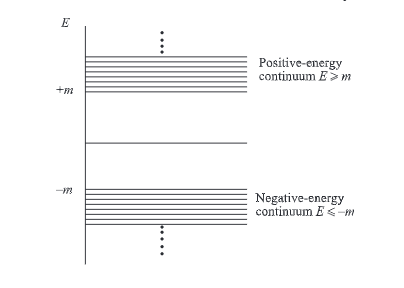
\includegraphics[width=0.65\linewidth]{mardedirac.png}
    \caption{Mar de Dirac }
    \label{fig:mardedirac}
\end{figure}
Dirac propone que el vació esta lleno de partículas de energía negativa o las anti-partículas. 

\begin{align*}
    e^- +e^+ \\
    E'+E \geq 2m
\end{align*}
En 1934 Pauli y weisskoff, proponen: 
\[
\mathcal{J}^\mu = -i \text{e}(\phi ^*\partial ^\mu \phi -\phi \partial^\mu \phi^*) \hspace{3ex} \phi' \to e^{iq x} \phi \hspace{3ex} x =x(\Vec{x},t)
\]
$\rho = \mathcal{J^0}$ 
\begin{align*}
    \mathcal{J}^{\mu } (e^-) &= -2e \abs{N}^2(E, \Vec{ P}) \hspace{4ex} \text{ Partícula} \\
\mathcal{J}^{\mu } (e^+) &=  2e \abs{N}^2(E, \Vec{ P}) \hspace{4ex} \text{Anti-Partícula} \\    
\uparrow e^+ &\equiv \quad \downarrow e^- \\
E>0 &\quad (-E) >0\\
\to e^{-i (-E) (-t)} &= e^{-Et} 
\end{align*}

\underline{Punto crucial:} Hay diagramas que corresponden a la misma observacón, en los que vamos a incluir todos los posibles ordenamientos temporales: 



\subsection{La ecuación de Dirac} 

Escribir una ecuación lineal: 
\[
E^2= \Vec{P} ^2+\not m^0
\]
K-G
\[
E\to \partial_t \hspace{5ex} \Vec{P} \to -i\nabla  \hspace{5ex} m=0
\]
La propuesta de Dirac es:
\[
H \psi = (\Vec{\alpha} \cdot \Vec{ P} +\beta m) \psi \quad \checkmark
\]
pero, ¿Cómo determino $\Vec{\alpha }$ y $\beta$ ?
\begin{align*}
    H^2\psi &=(\Vec{P} +m^2 ) \psi \\
    &= (\alpha_i P_i+\beta m )( \alpha_jPj+\beta m) \psi\\
    &= (\alpha_iP_i\alpha_jP_j +\alpha_iP_i \beta m+ \beta m \alpha_j P_j +\beta^2m ^2  ) \psi \\
    &= (\alpha_i^2 P_i ^2+\underbrace{\alpha_i \alpha_j P_i Pj \big|_{i\not = j} }_{(\alpha_i\alpha_j +\alpha_j\alpha_i)P_iP_j|_{i>j}  } +( \alpha_i \beta +\beta \alpha_i) P_i m +\beta^2m ^2 ) \psi
\end{align*}
Veamos que esto es ciero, si tomo $i = j $ y $i \not =j$ 
\[
\alpha_i^2=\mathbb{I} \quad \& \quad \beta^2 = \mathbb{I}
\]
Tomando al anti-conmutador como: 
\begin{align*}
    \alpha_i \beta +\beta \alpha_i &=0\\
    \{ \alpha_i, \beta\} &=0
\end{align*}
Para la otra parte, si tomamos: 
\begin{align*}
    \alpha_i\alpha_j P_iP_j \big |_{i =j } &= (\alpha_i\alpha_j+ \alpha_j\alpha_i )P_iP_j \big|_{i<j } \\
\end{align*}
Con las combinaciones correspondientes:
\[
 \begin{array}{cc}
      i&j  \\
      1& 2 \\
      1&3\\2&1\\2&3\\3&1\\3&2
 \end{array}
\]
\[
\Rightarrow \{\alpha_i, \alpha_i\} =0
\]
Necesitamos que:
\[
H^2\psi = (\Vec{P}^2+ m ^2 ) \psi 
\]
Entoces, tenemos las siguientes condiciones: 
\begin{itemize}
    \item $\alpha_i^2 = \mathbb{I}$ implica que $\alpha_1,\alpha_2,\alpha_3,\beta $ anti conmutan
    \item $\alpha_i\alpha_j + \alpha_j\alpha_i =0$ implica que $\alpha_1^2=\alpha_2^2=\alpha_3^2=\beta ^2= \mathbb{I}$
    \item $\alpha_i \beta +\beta \alpha_i =0$ 
    \item $\beta ^2= \mathbb{I}$ para $i=1,2,3$ 
\end{itemize}

\begin{tcolorbox}[colback=yellow!10, colframe=red!20!black, title=Tarea ] 
 Mostrar que las propiedades de $\alpha_i$ y $\beta $ son:

 \begin{enumerate}
     \item Hermíticas 
     \item  Traza 0 
     \item  Dimensión par 
     \item  Autovalores $+1$ y $-1$ 
 \end{enumerate}
\end{tcolorbox}
\fbox{

\begin{minipage}{0.9\textwidth}
\underline{Solución}
\begin{enumerate}
    \item \textbf{Hermiticidad: }
Ya que sabemos que la ecuación de Dirac tiene la forma:
\[
H \psi = \qty(\Vec{\alpha } \cdot \Vec{ P}+ \beta m   ) \psi 
\]
Queremos que el hamiltoniano $H$ deba de ser Hermítico, para garantizar una evolución unitaria y probabilidades reales. Entonces, el momentum $P = -i \nabla$ y la masa $m$ son reales y por tanto hermíticos,  debemos requerir que las matrices $\alpha_i , \beta $ sean hermíticas, es decir:
\[
\alpha_i ^\dagger = \alpha_i\quad, \quad \beta^\dagger =\beta 
\]
Entonces:
\begin{align*}
    H^\dagger &= \qty(\Vec{\alpha }\cdot \Vec{P } +\beta m )^\dagger\\
    &= \Vec{\alpha }^\dagger \cdot \Vec{\alpha }^\dagger +\beta ^\dagger m^\dagger=\Vec{\alpha }\cdot \Vec{P } +\beta m  =H.
\end{align*}
Por lo tanto, cada uno de los operadores es Hermítico.
\item  \textbf{Traza 0} 


De lo visto anteriormente, sabemos que las matrices $\alpha_i , \beta$ satisfacen las relaciones de anti-conmutación:
\[
\alpha_i, \beta  = 0
\]
Podemos aprovechar esto y tomar que:
\[
\alpha_i \beta =- \beta \alpha_i
\]

Entonces, tomando su traza y aplicando la propiedad ciclica de la traza: $Tr(AB) = Tr(BA)$, tenemos:
\begin{align*}
    Tr(\alpha_i \beta ) &= -Tr(\beta\alpha_i  )\\
    \Rightarrow 2Tr(\alpha_i \beta ) &=0 \\
    \Rightarrow Tr (\alpha_i \beta) &=0.
\end{align*}
Ahora, manipulemos la expresión de anticonmutación un poco, multiplicando por $\beta$ 
\begin{align*}
    \alpha_i \underbrace{\beta\cdot \beta }_{\mathbb{I}} &=-\beta \alpha_i \beta \\
    \Rightarrow Tr(\alpha_i) &=  - Tr(\beta \alpha_i \beta  ) \\
    Tr(\alpha_i) &=-Tr( \alpha_i \beta^2 )=-Tr(\alpha_i)  \Rightarrow Tr(\alpha_i)  =0
\end{align*}
De forma análoga podemos hacer lo mismo para $\beta$ para obtener también que:
$Tr(\beta  ) =0$.

\end{enumerate}


\end{minipage}
}

\fbox{
\begin{minipage}{0.9\textwidth}
\begin{enumerate}
\item  \textbf{Dimensión par}

Sabemos que la dimensión más pequeña es de matrices de $4\times 4$, aunque solo tenemos 3 matrices de pauli, la cuarta se formaría como una combinación lineal de las matrices de pauli. 

 dado que nos adelantas que solo podemos tener dos valores propios posibles $\pm 1$ y que además, ya vimos que su traza es cero. Entocnes, eel número de valores propios $+1$ debe ser igual an número de valores propios $-1$. 
 Entonces, si interpretamos la dimensión $n$ que es el número total de valores propios esta debe ser par: $n=2k $

Esto no se puede resolver con algebra lineal con el teorema de rango nulidad: 
\[
\text{dim}( Ran T)+\text{dim}(Ker(T)) = \text{dim} V
\]
Porqué no aborda las relaciones entre las matrices de anti conmutación y no podemos forzar a que la matriz $\beta$  anticonmute econ toas las matrices de pauli $\sigma_i$.

Lo correcto sería hacerlo con el álgebra de Clifford.

Donde los generadores serían $\alpha_i, \beta$, de esta tendríamos una metríca que tiene una dimensión minima para 4 generadores que anticonmutan igual a 4. 

Esta es la reprecentación \textbf{Pauli- Dirac} que se ve en la siguiente pagina.


\item \textbf{Autovalores $+1,-1$}

En esta podemos hacer uso de las propiedades:
\[
\alpha_i^2= \mathbb{I} \hspace{5ex} \& \hspace{5ex} \beta^2= \mathbb{ I}
\]
En esta, trabajandolo con álgebra lineal, podemos tener que: por ejemplo, sii tenemos una matriz $M$ con $M^2=\mathbb{ I}$ su polinomio característico es:
\[
\lambda^2-1 =(\lambda-1)(\lambda+1) =0
\]
Y de ello sus valores y vectores propios serían $\lambda = \pm 1 $

Entonces, usando esto, se tiene que: para cualquier valor propio $\lambda $ de $\alpha_i $, tenemos:
\begin{align*}
    \alpha_i v &= \lambda v \Rightarrow \alpha_i^2v = \lambda^2v=v\\
    \Rightarrow \lambda^2&=1 \\
    \Rightarrow \lambda &= \pm 1
\end{align*}

 y analogamente para $\beta$ . 
\end{enumerate}
\end{minipage}

}

La representaciín \textbf{Dirac-Pauli} 
\[
\alpha_i =\begin{pmatrix}
    0 & \vdots&\sigma_i\\\cdots& &\cdots \\\sigma_i & \vdots &0
\end{pmatrix} \hspace{3ex}, \quad \beta = \begin{pmatrix}
    \mathbb{I}_{2\times2} & \vdots&0\\\cdots& &\cdots \\0 & \vdots &\mathbb{I}_{2\times2} 
\end{pmatrix} \quad \checkmark
\]
Representación de Weyl
\[
\alpha_i =\begin{pmatrix}
    -\sigma_i & \vdots&0\\\cdots& .&\cdots \\0 & \vdots &\sigma_i
\end{pmatrix} \hspace{3ex}, \quad \beta = \begin{pmatrix}
    0 & \vdots& \mathbb{I}_{2\times2}\\\cdots& .&\cdots \\\mathbb{I}_{2\times2} & \vdots &0
\end{pmatrix} \quad \checkmark
\]

\begin{tcolorbox}[colback=yellow!10, colframe=blue!20!black, title=Tarea ] 
 Mostrar que la representaciones de Pauli-Dirac y la representacón de Weyl cumplen con las características de la las matrices $\alpha_i, \beta $
\end{tcolorbox}
\fbox{

\begin{minipage}{0.9\textwidth}
\underline{Solución}

\end{minipage}
}

\subsection{Solución a la ecuación de Dirac}

\begin{align*}
    H &= \Vec{\alpha } \cdot \Vec{P} +m \beta \\
    i \frac{\partial  \psi }{\partial t } &= \qty(-i \Vec{\alpha }\cdot \nabla + \beta m  ) \psi \\
\text{ Multiplicamos por } \beta \\
    \qty( i \beta \frac{\partial   }{\partial t }  + i \beta \Vec{\alpha }\cdot \nabla - m  ) \psi &=0  \\
    \gamma ^\mu &=(\beta, \beta\Vec{\alpha } )  \quad (\gamma_{ ij})^\mu \\
    \qty(i \gamma^\mu \partial_\mu  -m   ) \psi &= 0 \hspace{2ex} \text{Notación} \quad \not A=\gamma^\mu A_\mu \\
    (i \not \partial -m )\psi &=0 
    \end{align*}
Donde \[
(\gamma_{ij})^\mu A_\mu= (\gamma_{ij})^0 A_0 +(\gamma_{ij} )^1A_1+(\gamma_{ij})^2A_2
\]
Se tiene:
\[
\sum_k \qty[\sum_\mu i (\gamma^\mu )_{jk} \partial _\mu - m \delta_{jk }   ] \psi_k =0\quad \phi' (x' ) =\phi(x)
\]

La representación \textbf{Dirac-Pauli} es de nuevo:
\[
\alpha_i =\begin{pmatrix}
    0 & \vdots&\sigma_i\\\cdots& &\cdots \\\sigma_i & \vdots &0
\end{pmatrix} \hspace{3ex}, \quad \beta = \begin{pmatrix}
    \mathbb{I}_{2\times2} & \vdots&0\\\cdots& &\cdots \\0 & \vdots &\mathbb{I}_{2\times2} 
\end{pmatrix} \quad \checkmark
\]

\begin{tcolorbox}[colback=yellow!10, colframe=blue!20!black, title=Tarea ] 
 Mostrar que  
\[
\gamma^\mu \gamma^\nu +\gamma^\nu \gamma^\mu =2 \eta^{\mu\nu }
\]

 $\gamma^\mu =\{ \beta, \beta\Vec{\alpha} \}$
\[
\gamma^0= \beta \quad(\gamma^0) ^+ = \gamma^0 \quad (\gamma^0)^2  =1
\]
$k=1,2,3$ $\gamma^k = \beta \alpha ^k $ $(\gamma^k )^+=(\beta\alpha^k)^+ =\alpha^k \beta =- \beta \alpha^k=-\gamma ^k  $ 
\[
(\gamma^k)^2=(\beta\alpha^k\beta\alpha^k)  = - \beta^2 \alpha^{k^2 } =-\mathbb{I}
\]
 \begin{align*}
     (\gamma^\mu ) ^+&= \gamma^0\gamma^\mu \gamma^0 \\
     (\gamma^\mu)^+  &= \gamma^0\gamma^i\gamma^0 =-\gamma^0\gamma^0 \gamma^i =- \gamma^i 
 \end{align*}

 
\end{tcolorbox}
\fbox{

\begin{minipage}{0.9\textwidth}
\underline{Solución}

\end{minipage}
}
\subsubsection{La ecuación de continuidad $\partial_m \mathcal{J}^\mu =0 $}


\[
i \gamma^0\frac{\partial \psi^+}{\partial t } -i \frac{\partial \psi }{\partial x^k } (-\gamma ^k)- m \psi^+=0
\]


El hamiltoniano conjudado:
\[
-i \frac{ \partial \psi^\dagger}{\partial t } \gamma^0 - i \frac{\partial \psi ^\dagger}{ \partial x^k} (\gamma^k)   - m \psi^\dagger  =0
\]
Multiplicando por $\gamma^0 $ 


\[
-i \frac{ \partial ( \gamma^0)}{\partial t } \gamma^0 + i \frac{\partial \psi ^\dagger}{ \partial x^k} \gamma^k \gamma^0 - m \psi^\dagger \gamma^0=0
\]
 Espinor adjunto $\overline{\psi} = \psi^\dagger \gamma^0$  
 \begin{align*}
     -i \frac{\partial \overline{\psi}}{ \partial t} \gamma^0-i \frac{ \partial \overline{\psi}}{ \partial x^k} \gamma^k - m \overline{\psi} &=0  \\
     i \partial_\mu \overline{ \psi} \gamma^\mu +m \overline{\psi} &=0.
 \end{align*}
\begin{tcolorbox}[colback=yellow!10, colframe=blue!20!black, title= Ejercicio ] 

 Mostrar que la ecuación de continuidad tiene la forma 
 \[
 \partial_\mu \underbrace{(\overline{\psi }\gamma^\mu \psi   )}_{\mathcal{J}^\mu }  =0
 \]
 \[
 \rho = \mathcal{ J^0} = \overline{\psi} \gamma ^0 \psi= \psi^\dagger \gamma^0\gamma^0\psi = \abs{\psi}^2 = \sum_i  \abs{\psi_i}^2
 \] 
\end{tcolorbox}
\fbox{

\begin{minipage}{0.9\textwidth}
\underline{Solución}

\end{minipage}
}
\begin{tcolorbox}[colback=yellow!10, colframe=blue!20!black, title=Ejercicio ] 
 Mostrar que operando $\partial^\mu \partial_\nu$ en la ecuación de Dirac cada componente satisface la ecuación de Klein-Gordon
 \[
 (\square +m^2)\psi_i =0
 \]
\end{tcolorbox}
\fbox{

\begin{minipage}{0.9\textwidth}
\underline{Solución}

\end{minipage}
}

Regresando a la ecuación de Dirac: 
\[
i \frac{\partial }{\partial t } \psi  = \left\{ 
-i \qty(\alpha^1 \frac{\partial }{\partial x'  }+\alpha^2 \frac{\partial }{\partial x^2 }+\alpha^3 \frac{\partial }{\partial x^3 }   ) + \beta m \right\} \psi 
\]
\[
\to \psi(\Vec{x} , t) = Nu(P) \underbrace{\text{exp}[ -i ( P\cdot t - \Vec{P} \cdot \Vec{x})]}_{\text{exp}(-i P^\mu \mathcal{X}_\mu )  }
\]
Sustituyendo: 
\begin{align*}
    (\alpha_1 P_1+ \alpha_2 P_2+ \alpha_3 P_3 +\beta m) u - P^0u =0
\end{align*}
\[
u = \begin{pmatrix}
    a\\b\\\dots\\f\\g
\end{pmatrix} \hspace{3ex} \Vec{\alpha} = \begin{pmatrix}
    0 & \vdots &\sigma\\\cdots&.&\cdots \\ \sigma &\vdots&0
\end{pmatrix} \hspace{3ex} \beta = \begin{pmatrix}
    \mathbb{I }& \vdots &0 \\
    \cdots &.&\cdots\\ 0&\vdots&- \mathbb{I}
\end{pmatrix}
\]

\begin{align*}
    \begin{pmatrix}
        \mathbb{I}m-\mathbb{I}{p_0}&\vdots &\sigma_1 P_1+\sigma_2P_2+\sigma_3P_3 \\\cdots & .& \cdots\\
        \sigma_1 P_1+\sigma_2P_2+\sigma_3P_3 & \vdots&-\mathbb{I}m-\mathbb{I}{p_0}
    \end{pmatrix} \begin{pmatrix}
        a\\b  \\\_ \\f\\g
    \end{pmatrix} &=
\end{align*}

\[
\begin{pmatrix}
    m-P_0 &0 & \vdots& P_3& P_1-i P_2 \\
    0 & m-P_0 &\vdots &P_1+iP_2 &-P_3\\
    \cdots &\cdots&. &\cdots& \cdots \\
    P_3 & P_1-iP_2 &\vdots& -(m+P_0) &0\\
    P_1+iP_2&-P_3 &\vdots &0 & -(m+P_0)
\end{pmatrix} \begin{pmatrix}
    a\\b\\\_\\ f\\g
\end{pmatrix}
\]


\begin{tcolorbox}[colback=yellow!10, colframe=blue!20!black, title=Ejercicio ] 
  Calcular el determinante de la matriz anterior. 

  Dobo llegar a: 
  \[
  det[ (.)]  = [m ^2-(P^0)^2+(\Vec{ P})^2]^2 
  \]
\end{tcolorbox}
\fbox{

\begin{minipage}{0.9\textwidth}
\underline{Solución}

\end{minipage}
}
Si el determinante $det(4\times 4) =0$, el sistema no tiene solución porque  existe una relación entre las componentes $a:b:f:g$ 
\begin{tcolorbox}[colback=yellow!10, colframe=blue!20!black, title=Ejercicio ] 
  Calcular el determinante de las matrices menores $\to$ también tiene la forma $(P^0)^2-m^2-(\Vec{P})^2=0. $
\end{tcolorbox}
\fbox{

\begin{minipage}{0.9\textwidth}
\underline{Solución}

\end{minipage}
}
Unicamente 2 de las 4 componentes del espinor son independientes.

Sabiendo que esta relación se debe de cumplir, tenemos dos casos:

\underline{Caso (A)} 

\begin{align*}
    P^0&=(m^2+ \Vec{P}^2 )^{1/2 } \\
    \left\{-(m^2+ \Vec{P}^2 )^{1/2 }+m  \right\}a +P^3 f+(P_1-iP_2)g&=0 \\
    \left\{-(m^2+ \Vec{P}^2 )^{1/2 }+m  \right\}b + f(P_1-iP_2) -P^3 g&=0
\end{align*}
Si fijo dos de ellos, hago la propuesta:

\begin{enumerate}
    \item \[
    a=1,\quad b =0 
    \] 
    \item  \[
    a=0, \quad b=1
    \]
    Entonces
\end{enumerate}
\[
f= \frac{P_1 }{ (m^2+ \Vec{P}^2 )^{1/2 } +m} , \hspace{4ex} g = \frac{P_1+ iP_2}{(m^2+ \Vec{P}^2 )^{1/2 } +m }
\]

La constante de noramalización:
\[
W_1 = N \begin{pmatrix}
    1\\0\\\_\\ \frac{P_1 }{ (m^2+ \Vec{P}^2 )^{1/2 } +m}\\ \frac{P_1+ iP_2}{(m^2+ \Vec{P}^2 )^{1/2 } +m }
\end{pmatrix}
\]
y haciendo lo mismo para la segunda opción, el segundo espinor es:
\[
W_2 = N \begin{pmatrix}
    1\\0\\\_\\  \frac{-P_1- iP_2}{(m^2+ \Vec{P}^2 )^{1/2 } +m } \\\frac{-P_1 }{ (m^2+ \Vec{P}^2 )^{1/2 } +m}
\end{pmatrix}
\]

Repetri para $P^0 = -(m^2 \Vec{P}^2  )^{1/2} $, partiendo que la energía es negativa. 
Donde escogemos las componentes $f=0, g=1$ 
\[
W_3 = N \begin{pmatrix}
     \frac{P_1- iP_2}{(m^2+ \Vec{P}^2 )^{1/2 } +m } \\\frac{P_1 }{ (m^2+ \Vec{P}^2 )^{1/2 } +m} \\ \_ \\0 \\1
\end{pmatrix} 
\]
\[
W_1 = N \begin{pmatrix}
     \frac{-P_3 }{ (m^2+ \Vec{P}^2 )^{1/2 } +m}\\ \frac{-(P_1+ iP_2)}{(m^2+ \Vec{P}^2 )^{1/2 } +m } \\\_\\1\\0
\end{pmatrix}
\]
Esta fue la forma explicita, pero vamos a repetir lo mismo, haciendolo por bloques de 2$\times$ 2. 
Proponemos una solución:
\begin{align*}
    \psi&=u (P) e^{iPx} \\
    (\partial^\mu P_\mu -m ) u(P)&=0. \to (\not P -m  ) u=0.
\end{align*}
Encontramos los auto estados de energía para saber que es lo que nos estan representando, para ello despejamos el hamiltoniano:
\[
Hu( P) = (\Vec{\alpha }\cdot \Vec{P} + \beta m ) u = Eu
\]
En la representación de Pauli -Dirac $P=0$ esto se simplifica,  obtenemos directamente:
\[
H u = \beta m u = \begin{pmatrix}
    m \mathbb{I} &0\\ 0 &- m \mathbb{I} 
\end{pmatrix} u
\]

Veamos que tenemos 4 energías: $E=m,m_1,-m,-m_1$

Los que tienen energía positiva:
\[
\begin{pmatrix}
    1\\0\\0\\0
\end{pmatrix} \quad ,\begin{pmatrix}
    0\\1\\0\\0
\end{pmatrix} \hspace{3ex} E>0 \quad \text{Electrones}
\]
\[
\begin{pmatrix}
    0\\0\\1\\0
\end{pmatrix} \quad, \begin{pmatrix}
    0\\0\\0\\1
\end{pmatrix} \hspace{3ex} E<0 \quad \text{Positrones }
\]
Para $\Vec{P} \not =0$

\[
Hu = \begin{pmatrix}
    m & \Vec{\sigma} \cdot \Vec{P} \\\Vec{\sigma} \cdot \Vec{P}&-m
\end{pmatrix} \begin{pmatrix}
    u_A\\u_B
\end{pmatrix} =E \begin{pmatrix}
    u_A \\U_B
\end{pmatrix}
\]

Esto se reduce a :

\begin{align*}
     m u_A +\Vec{\sigma} \cdot \Vec{P} u_B &= Eu_A \hspace{3ex} \Vec{\sigma} \cdot \Vec{P} u_B = (E-m) u_A \tag{I} \\
     \Vec{\sigma} \cdot \Vec{P}u_A -mu_A &=E u_B \hspace{3ex} \Vec{\sigma} \cdot \Vec{P}u_A =(E+m)u_B \tag{II}
\end{align*}

Para soluciones de, $E>0$
\[
u_A^{(s)} = \mathcal{X}^{(s)}  , \quad \mathcal{X}^{(1)} = \begin{pmatrix}
    1\\0
\end{pmatrix} ,\quad \mathcal{X}^{(2)} = \begin{pmatrix}
    0\\1
\end{pmatrix}
\]
y despejando queda:
\[
u_B^{(s)} = \frac{\Vec{\sigma} \cdot \Vec{P} }{E+m } \mathcal{X}^{(s)} 
\]
\begin{tcolorbox}[colback=yellow!10, colframe=blue!20!black, title=Ejercicio ] 
 Mostrar 
 \[
 (\Vec{\sigma} \cdot \Vec{P})^2=\Vec{P}^2\mathbb{I}
 \]
\end{tcolorbox}
\fbox{

\begin{minipage}{0.9\textwidth}
\underline{Solución}

\end{minipage}
}




Tomando el espinor: $u^{(s)} = \begin{pmatrix}
    \mathcal{X}^{(s)}  \\ \frac{\Vec{\sigma} \cdot \Vec{P}} {E+m}
\mathcal{ X}^{(s)}\end{pmatrix}$


\begin{align*}
    E   \begin{pmatrix}
    \mathcal{X}^{(s)}  \\ \frac{\Vec{\sigma} \cdot \Vec{P} } {E+m}
\mathcal{ X}^{(s)} \end{pmatrix} &= \begin{pmatrix}
    m \mathbb{I} & \Vec{\sigma} \cdot \Vec{P}\\\Vec{\sigma} \cdot \Vec{P} &-m \mathbb{I}
\end{pmatrix} \begin{pmatrix}
    \mathcal{X}^{(s)}  \\ \frac{\Vec{\sigma} \cdot \Vec{P} } {E+m}
\end{pmatrix} \\
&=\begin{pmatrix}
    m \mathcal{X}^{(s)} +   \frac{\Vec{\sigma} \cdot \Vec{P} } {E+m}
\mathcal{ X}^{(s)} \\
  \Vec{\sigma} \cdot \Vec{P}\mathcal{ X}^{(s)}  - \frac{ m(\Vec{\sigma} \cdot \Vec{P} )} {E+m}
\mathcal{ X}^{(s)}
\end{pmatrix}
\end{align*}
De la primera componente: 
\[
m \mathcal{ X}^{(s)} + \frac{\Vec{P}^2 }{E+m }\mathcal{ X}^{(s)} =m\mathcal{ X}^{(s)} +\frac{E^2-m ^2}{E^2+m} \mathcal{ X}^{(s)}
\]
\[
= m \mathcal{ X}^{(s)} +(Ee-m)\mathcal{ X}^{(s)}=E \mathcal{ X}^{(s)}
\]
para la seguna componente tenemos: 
\[
(\Vec{\sigma} \cdot \Vec{P}) \qty(1- \frac{m}{E+m} ) \mathcal{X}^{(s)} = (\Vec{\sigma} \cdot \Vec{P})\frac{(E+m-m) }{E+m} \mathcal{X}^{(s)} 
\]
\[
= E\frac{\Vec{\sigma} \cdot \Vec{P}}{ E+m} \mathcal{X}^{(s)}
\]
Para $E<0$
 Repetimos el mismo procedimiento, pero esta vez tenemos:


 \[
  u_B^{(s)} = \mathcal{X}^{(s)} \to u_A = \frac{\Vec{\sigma} \cdot \Vec{P}}{E-m }u_B = -\frac{\Vec{\sigma} \cdot \Vec{P}}{\abs{E}+m  }  \mathcal{X}^{(s)}
 \]

y obtenemos:
\[
u^{(s)} =N \begin{pmatrix}
    \mathcal{X}^{(s)}  \\\frac{\Vec{\sigma} \cdot \Vec{P}}{E+m}  \mathcal{X }^{(s)}  
\end{pmatrix} \hspace{3ex} u^{(s) }= N \begin{pmatrix}
    - \frac{\Vec{\sigma} \cdot \Vec{P}}{\abs{E +m } } \mathcal{X}^{(s)} \\
    \mathcal{X}^{(s)}
\end{pmatrix}
\]
\[
\mathcal{X}^{(s)}  \to \mathcal{X}^1 = \begin{pmatrix}
    1\\0
\end{pmatrix} \quad \mathcal{X}^2 = \begin{pmatrix}
    0\\1
\end{pmatrix}
\]
\begin{tcolorbox}[colback=yellow!10, colframe=blue!20!black, title=Ejercicio ] 
 Verificar que los 4 espinores son ortogonales:
 \[
 u^{(s )\dagger } + u^{(r)} =0 , \quad r\not =s
 \]
\end{tcolorbox}
\fbox{

\begin{minipage}{0.9\textwidth}
\underline{Solución}

\end{minipage}
}
Un operador que rompa la degeneración 
\[
\Sigma\cdot \hat{P} = \begin{pmatrix}
    \Vec{\sigma} \cdot \hat{P}  & 0\\0&\Vec{\sigma} \cdot \hat{P} 
\end{pmatrix}, \quad \hat{P}  = \frac{\Vec{P}}{\abs{\Vec{P}} }
\]

\begin{tcolorbox}[colback=yellow!10, colframe=blue!20!black, title=Ejercicio ] 
 Verificar que $\Sigma \cdot \hat{P}$ conmuta con $H$ 
\end{tcolorbox}


\subsubsection{Helicidad: }

La proyección del espín en la dirección del momento, la defino como: 
\[
\frac{1}{2} \Vec{\sigma} \cdot \hat{P} 
\]
\[
\lambda = \begin{cases}
    \frac{1}{2} \quad \text{ Helicidad positiva } \quad \Rightarrow \\
    -\frac{1}{2} \quad \text{ Helicidad Negativa} \quad \Leftarrow 
\end{cases}
\]
Recordemos que: 
\[
X^{1} = \begin{pmatrix}
    1\\0
\end{pmatrix}\quad X^2 = \begin{pmatrix}
    0\\1
\end{pmatrix}
\]

Para $\Vec{P}=(0,0 , P) $ 
\[
\frac{1 }{2} \sigma\cdot \hat{P} X^3= \frac{1 }{2} \sigma_3\cdot \hat{P} X^{(s)} = \begin{pmatrix}
    1/2 &0\\0&-1/2
\end{pmatrix}
\]

\begin{tcolorbox}[colback=yellow!10, colframe=blue!20!black, title=Ejercicio ] 
 Calcular el espinor de helicidad $1/2$ para un electrón con momento $P =(P \cos\theta, 0, P \sin \theta)$
\end{tcolorbox}
¿Es la helicidad un buen numero cuántico ? 

Es un buen número cuántico cuando hablamos de partículas sin masa.
\begin{tcolorbox}[colback=yellow!10, colframe=blue!20!black, title=Ejercicio ] 
Confirmar que la ecuación de Dirac describe partículas con momento angular intrínseco $\frac{1}{2}$ (espín $1/2$) 

\begin{enumerate}
    \item Usando el conmutador $[x_i, P_j  ] = i \delta_{ij} $ mostrar
    \[
    [H,L]= -i (\Vec{\alpha } \times \Vec{P} ) 
    \]

    \item  \[
    \Sigma = \begin{pmatrix}
        \sigma &0 \\0 &\sigma
    \end{pmatrix} \hspace{5ex} [H, \Sigma] =2i(\Vec{\alpha}\times \Vec{P} )
    \] 
    \item  $J = L+ \underbrace{1/2 \Sigma} $ El operador de espín. 
    \[
    [H, J] =0
    \]
\end{enumerate}
 
\end{tcolorbox}

\subsection{Teoría de Perturbaciones No relativistas} 
Partícula libre independiente del tiempo. 

\[
\to H_0  \phi _n= E_n \phi_n 
\]
\[
\int d  ^3z \phi_n \phi_ m^* = \delta_{nm}
\]
En presencia de $V$, en notación de Schrodinguer:
\[
(H_0 +V(\Vec{x}, t))\psi = -i \frac{ \partial \psi}{ \partial t } \hspace{5ex}|\quad  V(\Vec{x}, t) = \lambda  H'
\]
La solución; 
\[
\psi = \sum_n a_n(t) \phi _n (\Vec{x}) \text{e}^{-i E_n t} 
\]
Sustituyendo:
\begin{align*}
    (H_0+ V(\Vec{x}, t)) \sum_n a_n(t) \phi _n (\Vec{x} ) e^{-i E_n t} &= i \sum_n   \frac{ d a_n(t)}{dt} \phi _n (\Vec{x} ) e^{-i E_n t}+\sum_n E_n a_n(t) \phi _n (\Vec{x} ) e^{-i E_n t}\\
    i \sum_n \frac{d a_n(t)}{dt }\phi _n (\Vec{x} ) e^{-i E_n t} &= \sum_n V(\Vec{x}, t)a_n(t)\phi _n (\Vec{x} ) e^{-i E_n t}
\end{align*}

Multiplicamos por $\phi_f ^*$ y integando $\int d^3x$ 
\begin{align*}
    i \sum_n \frac{d a_n(t)}{dt } e^{-i E_n t} \int \underbrace{d^3x \phi^*_f\phi _n (\Vec{x} ) }_{\delta_{nf}}   &= i \frac{d a_f(t)}{ dt} e^{-iE_f t} \\
    \frac{d a_f(t)}{dt} &= -i \sum_n a_n (t) \int d^3 x \phi _f^* (\Vec{x} )\phi_n e^{-i(E_f-E_n )t}. 
\end{align*}
\begin{align*}
    (H_0 +V(\Vec{x} ,t)) \psi &= i \frac{\partial \psi }{\partial t  } \hspace{5ex }|\quad H_0\phi_n = E_n \phi_n \\
    \to \psi &=  \sum_n a_n (t) \phi_n (x) e^{-i E_n t} \hspace{4ex} |\quad \int d^3 x \phi^* _n \phi_m = \delta _{nm} \\
    \rho &= \psi^*\psi = \qty(\sum_n a_n^*(t) \phi_n^* (\Vec{x})e^{i E_n t} ) \qty(\sum_m a_m (t) \phi_m (x) e^{-i E_m t})\\
    &= \sum_n\sum_m a_n^*a_m \phi_n^*\phi_m e^{i E_n t-iE_m t } \\
    P &= \int d^3 x \rho =\sum_{m,n }a_n^*a_m \int d^3x \phi_n ^*\phi_m e^{i E_n t-iE_m t } \\
    &= \sum_n \abs{a_n} ^2
\end{align*}
\[
\frac{d a_f (t)}{dt } = -i \sum_n a_n(t) \int d^3 x \phi_f^* V(\Vec{x}, t) \phi_n (\Vec{x}) e^{i  (E_f -E_i)t }. 
\]

\[
H = H_ 0+V(\Vec{x }, t) =\underbrace{ H_0 + \lambda H '}_{\text{Muy pequeño }}
\]

Vamos a considerar, que el potencial es pequeño, perturbativo y transitorio. 

Siguiendo Halzen, tomando $t=(-\tau/2 , \tau/2)$ 

A primer orden, tomando $t_{inicial} =-T/2$ 
\[
a_i (-T/2 )=1 
\]
\[
a_n(-T/2) =0\quad, \quad n \not= i 
\]


    \hspace{1cm}\begin{tikzpicture}[remember picture, overlay]
\node [circular drop shadow={shadow scale=1.05},minimum size=1cm,
decorate, decoration=zigzag,
fill=gray!20,draw,thick,circle] (A) {. };
\draw[arrows=->] (-0.5,-0.8)--(A.center);
\draw[arrows=->] (A.center) --(1.5,0.5); 
\node[] at (-0.6, -0.6 ) {$i$};
\node[] at (1.3,0.1) {$f$};
\node[] at (-1.3, 1) {Interacción de tipo: };
\fill (0,0) circle (1pt); 
\end{tikzpicture}
 \[
 \frac{d a_f}{dt} = -i \lambda  \int_v d^3x \phi^*_f \underbrace{V(\Vec{x,t})}_{\lambda H'} \phi_i e^{i (E_f-E_i)t}
 \]

\begin{align*}
    \int_{-T/2}^{t' } dt a_f (t) &= - i \int_{-T/2}^{t'} dt\int _v d^3 x \phi_f^* V(\Vec{x}, t ) \phi _i e^{i (E_f-E_i) t} \\
    \to a_f (t' )-a_f(\not^0 T/2^) &= - i \int_{-T/2}^{t'} dt\int _v d^3 x [\phi_f e^{-i E_f t} ]^* V(\Vec{x}, t ) \phi _i e^{-i E_i t} \\
    t_f = T/2 \\
    \to T_{fi} ^{(1)} = a_f^{(1)} &= - i \int_{-T/2}^{t'} dt'\int _v d^3 x [\phi_f e^{-i E_f t} ]^* \underbrace{V(\Vec{x}, t )}_{\lambda H'(x,t)} [\phi _i e^{-i E_i t}] \\
    &= -i \int d^4 x\phi^*_f(x)V(x) \phi (x)
\end{align*}
Válido solo sí, $a_f(t) \ll 1 $

\[
\to \abs{T_{f_i}^{(1 )} }^2 = \abs{a_f^{(1)} }  ^2 =\text{ Probabilidad Transición}
\]
Considerar un potencial independiente del tiempo: $T \to \infty:$ 

\[
T_{fi} -i V_{fi } \int_{-\infty }^\infty dt e^{i(E_f-E_i) t} ,\quad V_{fi} = \int d^3 x\phi^*_f(x) \underbrace{V(x)}_{\lambda H'} \phi_i(x)
\]
\[
= -i V_{fi }\delta(E_f-E_i)
\]
Es más útil definir la tasa de transición: 
\begin{align*}
    W &= \lim_{T\to \infty } \frac{\abs{T_{fi} }^2}{ T} \\
    W&= \lim_{T \to \infty  } \frac{ 2\pi \abs{V_{fi}}^2 }{T } \delta(E_f-E_i)\int_{-T/2} ^{T/2}e^{i (E_f-E_i )t}  dt
\end{align*}
Recordemos que: 
\[
\int d E_f \delta (E_f-E_i) e^{i(E_F-E_i)t}  =e^0
\]
Entonces: 
\begin{align*}
    W &= \lim_{T \to \infty} \frac{2\pi \abs{V_{fi} }^2 }{T} \delta (E_f -E_i) \underbrace{\int_{-T/2 }^{T/2}dt  }_{T} \\
    W&= 2\pi \abs{V_{if}}^2 \delta(E_f -E_i ) \\
    W_{fi} &= \int d_Ef \rho (E_f) W = 2\pi \abs{ V_{fi}}^2 \rho (E_i). \quad \text{ Regla de oro de Fermi.}
\end{align*}


\begin{align*}
    T_{ik} &= -i V_{ik}\int_0^T dt' e^{i \Delta E_{ki} t'  } =-\frac{V_{ki }}{\Delta E_{ki} } \qty(e^{i \Delta E_{ki} t} -1 ) \\
    T_{ki }&= -\frac{ V_{ki} }{\Delta E_{ki} } e^{\frac {i \Delta E_{ki} T}{2}} \underbrace{\qty(e^{\frac {i \Delta E_{ki} t }{2}  } -e^{\frac {i \Delta 
    E_{ki} T}{2}  })  }_{ 2\sin \qty(  \frac{\Delta E_{ki} t } {2}  )}    \\
    T_{ik }&= -\frac{2 V_{ ki} }{\Delta E_{ki} }  e^{\frac{i \Delta E_{ki} t}{2} } \sin\qty(\frac{\Delta E_{ki} t}{2} ) . \\
    P(i \to k) &= \frac{4 \abs{V_{ki } }^2 }{ (\Delta E_{ki})^2} \sin ^2\qty(\frac{\Delta E_{ki} t}{ 2} ). \quad \checkmark
\end{align*}



\begin{tikzpicture}
    % Configuración de ejes en pgfplots
    \begin{axis}[
        domain=-4*pi:4*pi,
        samples=280,
        axis lines=middle,
        xlabel={\large $\Delta E_{ki}$},
        ylabel={\large $P(i \to k) $},
        xmin=-4.3*pi, xmax=4.3*pi,
        ymin=0,      % Asumimos que la función >=0
        ymax=1.05,   % Para que sobresalga un poco la curva
        width=14cm,
        height=7cm,
        % Etiquetas en el eje x para -3\pi, -2\pi, -\pi, 0, \pi, 2\pi, 3\pi
        xtick={-3.14159*3, -3.14159*2, -3.14159, 0, 3.14159, 2*3.14159, 3*3.14159},
        xticklabels={$\frac{-3\pi}{t}$,$\frac{ -2\pi}{t}$,$-\frac{\pi}{t}$,0,$\frac{\pi}{t}$,$\frac{2\pi}{t}$,$\frac{3\pi}{t}$},
        tick label style={font=\large},
        label style={font=\large},
        legend style={at={(0.98,0.95)},anchor=north east}
    ]
    % Curva principal: sin^2((x)/2) como ejemplo
    % Puedes sustituir x por \Delta E_{ki} * t si deseas
    \addplot[thick,blue,domain=-4*pi:4*pi]
        {4*(sin(deg(x/2)))^2/x^2 }; 
    \addlegendentry{$\frac{4\abs{V_{ik} }^2 }{\Delta E_{ki}^2  } \sin^2\!\bigl(\tfrac{\Delta E_{ki}\,t}{2}\bigr)$}
        
    \end{axis}
\end{tikzpicture}

Pico
\begin{align*}
     \sin^2 (x) &=1, \hspace{3ex} x = \frac{\pi}{2} + n \pi \\
     \frac{\Delta E_{ik} t}{2} &=\frac{\pi }{2 } (1+2n ) \\
     \Delta E_{ki} &= \frac{\pi }{t} (2n +1 ) = (\frac{\pi}{t},\frac{3\pi}{t}, \frac{5\pi}{t} )
\end{align*}
Vertices:
\begin{align*}
    \sin^2(x) &=0\hspace{3ex} x = \pi m \\
    \Delta E_{ki} &= \frac{2 \pi m}{t } = (0, \frac{2\pi}{t},\frac{ 4\pi}{t}, \dots  )
\end{align*}

En los picos 
\begin{align*}
    P = \frac{4 \pi \abs{V_{ki}}^2 }{(\Delta E_{ki} )^2 } = \propto \frac{t^2}{\pi} \abs{V_{ki}}^2 
\end{align*}


\begin{tcolorbox}[colback=yellow!10, colframe=blue!20!black, title= Tarea ] 
 Mostrar que en la siguiente aproximación 
 \[
 T_{fi} = -2 \pi V_{fi} \delta  (E_f -E_i) -2\pi i \sum_{n \not=i} \frac{V_{fn}V_{ni} }{E_i-E_n +i \epsilon  } \delta (E_f-E_i )
 \]
 que en otras palabras 
 \[
 V_{fi} \to V_{fi }+ \sum_{n\not= i } V_{fn} \frac{1}{E_i -E_n +i \epsilon  } V_{ni} 
 \]
 
\end{tcolorbox}

\subsection{ Potencial que oscila en el tiempo: Radiación electro magnética.} 

Para incluir la presencia de un campo electro magnético: 
\[
P ^\mu \to P^\mu -e A^\mu 
\]
 Haciendo la sistitución o partiendo del  hamiltoniano clásico: 

 \[
 -\frac{1}{2m } \nabla^2\psi -\underbrace{\frac{i e}{m }\Vec{A}\cdot \Vec{\nabla }\psi -\frac{i e}{2m }\psi \nabla \Vec{A}+ \frac{e^2 \Vec{A}^2 }{ 2m}\psi       }_{V(x)} =E \psi 
 \]
Todo lo extra que me quede libre. porque es lo que puedo resolver con teoría de perturbaciones. 

Como el electromagnetismo es invariante gauge, El Gauge de Coulomb $\nabla\cdot \Vec{A } $ =0:
\[
V(x,t ) = -\frac{i e}{m } \overbrace{\Vec{A}}^{\text{fotones } } \cdot \nabla 
\]
Cuando hablamos de radiación electromagnética: \[
\nabla ^2 \Vec{ A }- \frac{1}{c^2}\frac{\partial ^2 A}{\partial t^2 }  =0 
\]

Con $A_0 = (a+ib) \Vec{\epsilon }$ , $\Vec{k} \cdot \Vec{\epsilon } =0$ 

\begin{align*}
    A(x,t) &= A_0 \text{exp} \{ i (\Vec{k} \cdot \Vec{\epsilon }- \omega t ) \}+A_0 ^*\text{exp} [ -i (\Vec{k} \cdot \Vec{\epsilon }-\omega t )], \quad \omega = c\abs{\Vec{k}} \\
    a_f^{(1)} (t) &=  \int_{t_0 }^t dt' V_{fi} (t') e^{i(E_f-E_i)t } \\
    V_{fi}&=\int d^3x \phi_f ^*V(\Vec{x} , t) \phi _i \\
    &=-\frac{ie}{m} \int d^3 x\phi _f ^* \{ \Vec{A} \cdot \nabla  \} \phi_i
\end{align*}
\begin{align*}
    V_{fi} (t) &= -\frac{i e}{m} \int d^3 x \phi _f ^* \left\{ \Vec{A}_0 e^{i \Vec{k} \cdot \Vec{x  }-i \omega t  }+ \Vec{A}_0^* e^{-i \Vec{k} \cdot \Vec{x  }+i \omega t  }   \right\}\cdot \nabla \phi  \\
    &= -\frac{i e}{m}  \left\{e^{-i \omega t   } \underbrace{\int d^3  x\phi_f^* e^{-i \Vec{k} \cdot \Vec{x  }  } A_0 \cdot \nabla \phi_ i }_{H_{fi}} + e^{i \omega t}  \underbrace {\int d^3x \phi_f ^*e^{i\Vec{k} \cdot \Vec{x  }  }A_0^* \cdot \nabla \phi_i  }_{H_{fi}^* }    \right\} \\
    &=- \frac{ie}{m } \left\{ e^{-i \omega t} H_{fi}+i e^{i\omega t} H_{fi}^*  \right\}
\end{align*}

Esto lo puedo reescribir como: 
\begin{align*}
    a_f^{(1)}(t) &= -\frac{e}{ m} H_{fi} \int_{t_0}^t dt' e^{-iwt }e^{i(E_f-E_i )t' } - \frac{e}{m}H_{fi}^*\int_{t_0}^tdt' e^{iwt' } e^{i(E_f-E_i)t' } \\
    \vdots \\
    a_f^{(1)}(t)&=\frac{2i \frac{e}{m }H_{fi}\sin[ (E_f-E_o w)t/2 ]  }{E_f-E_i -w} e^{i(E_f-E_i-w)t/2 }+ \frac{2ie }{ m} \frac{H_{fi}^* \sin [(E_f-E_i+w) t/2]  }{E_f-E_i+w} e^{ i( E_f-E_i +w)t/2 }
\end{align*}
A tiempos muy largos la probabilidad de transición es muy grande solo para 
\[
E_f-E_i -w =0 \tag{I}
\]
\begin{fmffile}{complex-a}
\begin{fmfgraph*}(150,100)
    \fmfleft{i1}
    \fmfright{o1,o2}
    \fmf{fermion,label=$e$ }{i1,w1}
    \fmf{photon,label=$\gamma $}{w1,o1}
    \fmf{fermion,label=$e$}{w1,o2}
     
    \fmfv{lab=Absorcion de un foton ,lab.dist=0.09w}{w1}
\end{fmfgraph*}
\end{fmffile}

\[
E_f= E_i +w 
\]
Y 
\[
E_f-E_i +w =0 \tag{ II}
\]
\[
E_f= E_i -w 
\]

\begin{fmffile}{emision-simple}
\begin{fmfgraph*}(150,80)
    \fmfleft{i1}
    \fmfright{o1,o2}
    \fmf{fermion}{i1,v1,o1} 
    \fmf{photon}{v1,o2}     
    \fmflabel{$e$}{i1}
    \fmflabel{$e$}{o1}
    \fmflabel{$\gamma$}{o2}
        \fmfv{lab=Emision de un foton ,lab.dist=0.09w}{v1}
\end{fmfgraph*}
\end{fmffile}
De la tarea para revisar el nivel de cuantica, a segundo orden: 
\[
V_{fi} = \int d^3 x \phi _{\rho }^* \underbrace{V(x)}_{\lambda H' }  \phi_i 
\]
\[
V_{fi} \to V_{fi} +\sum_{n\not= i } V_{fn} \frac{1}{E_i-E_n +i \epsilon }V_{ni}+ \cdots
\]
Dibujamos, asumiendo que $\uparrow$ el tiempo en la coordenada $y$  y $\to $ al espacio: 


 \begin{tikzpicture}[baseline=(current bounding box.center)]
    \begin{feynman}
        \vertex (i) {$i$} ;                  
        \vertex [right=2cm of i] (v1);        
        \vertex [above right=1cm of v1] (f) {\(f\)};  
        \vertex [right=2cm of v1] (plus) {\(+\)};     
        \diagram*{
            (i) -- [fermion] (v1) -- [fermion] (f),
        };      
        \draw[dashed] (v1) circle (0.5);
        \node[below=0.1cm] at (v1) {$V_{f1}$};
    \end{feynman}
    
    \begin{feynman}[shift={(5,0)}] % Desplazamiento horizontal
        \vertex (i) {\(i\)};
        \vertex [right =1.5cm of i] (v1);     
        \vertex [below right=0.5cm of v1] (v2);    
        \vertex [above right=1.5cm of v2] (f) {\(f\)};
        \diagram*{
            (i) -- [fermion] (v1) -- [fermion] (v2) -- [fermion] (f)  , 
        };
        \draw[dashed] (v2) circle (1.0);
        \node[above=0.1cm] at (v1) {$V_{f1}$};
        \node[below=0.1cm] at (v2) {$V_{f2}$};
    \end{feynman}
\end{tikzpicture}
En este arreglo notamos que: 
\begin{itemize}
    \item Por cada vértice aparece un término de interacción $\abs{V_{ni}} $ 
    \item Por la propagación de un estado intermedio aparece un propagador:
    \[
    \frac{1}{E_i -E_n  } 
    \] 
    \item  Los estados intermedios, partículas virtuales, no se conserva la energía en los vértices. 
\end{itemize}

\subsection{Mecánica Cuántica Relativista}



Formalismo de función de onda, $\rho$ muchas partículas: 
\[
\begin{array}{cc}
     \text{Partícula } & \text{anti-partícula }  \\
     \big \uparrow_{tiempo }  e^+ \quad \uparrow &  \equiv  \quad \downarrow \quad e^{-} 
\end{array}
\]
\subsection{Absorción de un fotón} 
\begin{center}
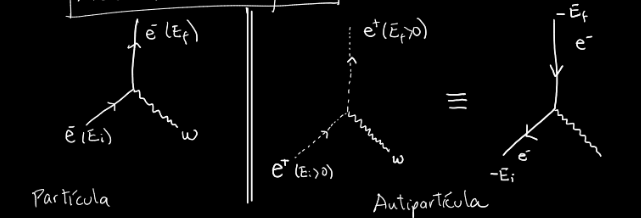
\includegraphics[width=12cm]{absorcionfoton.png}    
\end{center}
 
Volvamos a las ecuaciones de interacción de una partícula con Radicación: 

Partícula:
\[
\int dt (e ^{iE_f t})^* e^{-iwt } e^{-iE_i t}  \to 2\pi \delta (E_f -w -E_i )
\]
\[
E_f = E_i +w 
\]
Anti-Parícula
\[
\int dt  [e ^{-(-iE_f )t}]  ^* e^{-iwt } e^{-i( -E_f) t}  \to 2\pi \delta (-E_i -w +E_f )
\]
\[
E_f = E_i +w
\]
Una partícula cargada relativista en presencia de un potencial electromagnético: 


 Ecuación de Klein-Gordon,
\begin{align*}
    ( \partial^\mu \partial_\mu-m ^2  )\phi &=0 \hspace{3ex} \phi = \text{ sol. ec. de la partícula libre} \\
    \partial^\mu \to \partial^\mu +iq A^\mu  \\
    ( \partial^\mu \partial_\mu-m ^2  )\phi &=0\to [ ( \partial^\mu  -ieA^\mu    )(\partial_ \mu -ieA_ \mu ) - m^2  ]\phi =0\\
    [ \partial^\mu \partial _\mu -i e A^\mu \partial _\mu - ie\partial ^\mu A_\mu 
 -e^2 A^\mu A_\mu -m^2 ]\phi &=0
\end{align*}
Reescribiendo:
\[ 
[\partial ^\mu \partial _\mu -m ^2 ]\phi =-V\phi 
\]
\[
V= -i e (\partial _\mu A^\mu +A^\mu \partial _\mu ) - e^2A^2
\]
Despreciamos el término $\propto e^2$ 

\begin{tcolorbox}[colback=red!10, colframe=red!20!black, title=Tarea  ] 
 Mostrar que puedo resolverlo con teoría de perturbaciones. 
\end{tcolorbox}
\fbox{

\begin{minipage}{0.9\textwidth}
\underline{Solución}

\end{minipage}
}

\begin{align*}
    T_{fi} ^{1} &=- i \int d^4 x [ \phi_f e^{ -i E_f t}]^* V(x) [\phi_i e^{-iE_i t }]  \\ 
    T_{fi} ^{1} &=- i \int d^3 x dt \underbrace{[\phi_f e^{-iE_f t } ]^* }_{\varphi_f ^*} (A^\mu \partial_\mu +\partial_\mu A^\mu ) \underbrace{[ \phi_i e^{-i E_i t}  ]^*}_{\varphi_i} 
\end{align*}
Reescribiendo:
\[
\varphi_f^*\partial_\mu (A^\mu \varphi_i )  = \partial_\mu (\varphi_f ^* A^\mu \varphi_i ) - (\partial_\mu \varphi_f^* )A^\mu \varphi_i 
\]
Entonces, puedo escribir:
\[
\int d^4 x \varphi_f^*\partial_\mu (A^\mu \varphi_i  ) = - \int d^4x (\partial_\mu \varphi_f^* )A^\mu \varphi_i 
\]
Sustituyendo: 
\begin{align*}
    T_{fi } &= i (ie) \int d^4 x \left\{\phi^*_f A^\mu \partial_\mu \varphi_i   -(\partial_\mu \varphi_f^*  )A^\mu \varphi_i    \right\} \\ 
    &= -i \int d^4 x \mathcal{J}_\mu^{fi} A^\mu, \quad \mathcal{J}_\mu ^{fi} = -i e \{\phi_f^* (\partial_\mu \varphi_i   )-(\partial_\mu \varphi_f ^* )\varphi_i   \} 
\end{align*}
$\to \mathcal{J}_\mu ^{fi}:$ corriente de carga. 

\subsection*{21 de marzo}

\[
T_{fi}^{(1) } =- i \int d^4 x \qty[ \phi_f e^{-i E_f t}]^*V (x) [\phi_i e^{-iE_i t }]^*
\]
\[
T_{fi}^{(1) } =- i \int d^4 x \underbrace{\qty[ \phi_f e^{-i E_f t}]^*}_{\varphi_f ^* }\qty(A^\mu \partial_\mu +\partial_\mu A ^\mu  ) \underbrace{\qty[\phi_i e^{-iE_i t }]^*}_{\varphi_i }
\]

Reescribiendo esto: 
\[
\varphi_f^* \partial_\mu (A^\mu \varphi_i ) = \partial_\mu \qty(\varphi_f ^* A^\mu  \varphi_i  )- (\partial_\mu \varphi _f^* )A^\mu \varphi_i 
\]
Entonces, puedo escribir:


\begin{align*}
    T_{fi} &= i (ie) \int d^4 x \{  \phi_f^* A^\mu \partial_\mu \varphi_i - (\partial_\mu \varphi_f^*) A^\mu \varphi_i \} \\
    &= -i \int d^4 x \mathcal{J}_\mu ^{fi} A^\mu \quad, \quad \mathcal{J}_\mu ^{fi} = -ie \{ \phi_f^* (\partial_\mu \varphi_i ) - (\partial_\mu \varphi_f^*   )\varphi_i \} 
\end{align*}

$\to \mathcal{J}_\mu ^{fi}: $ Corriente de carga. 

\begin{minipage}{0.9\textwidth}
\begin{multicols}{2}  
    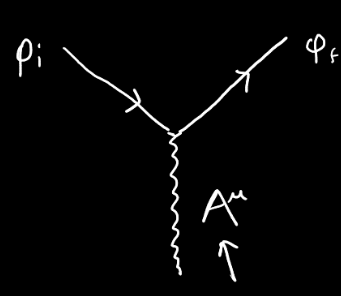
\includegraphics[width=8 cm]{0321.png}
 
 
\begin{align*}
    \varphi_i &= N_i e^{-i P_i \cdot x}\\
    \varphi_f &= N_f e^{-i p_f \cdot x } \\ 
    \mathcal{J}_\mu ^{fi} &= -e N_fN_i (P_i +P_f )_ \mu e^{i (P_f -P_i )\cdot x }
\end{align*}
\end{multicols}
\begin{multicols}{2}
    
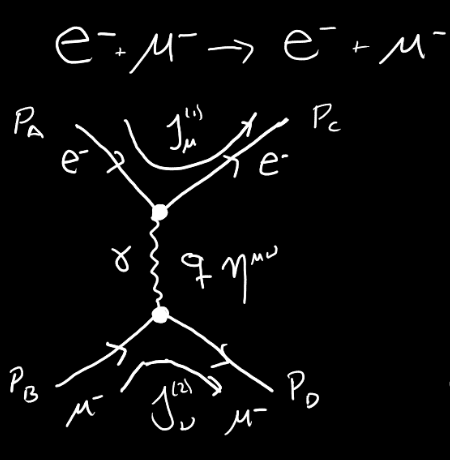
\includegraphics[width= 0.5 \textwidth ]{1321.png}

\begin{align*}
\to A+B \to C+D    
\end{align*}

Las ecuaciones de Maxwell
\[
\square A^\mu = J^\mu_{(2)} 
\]

\[
J_{(2)}^{\mu}  =- i e N_D N_B (P_D+P_B) e^{i (P_D -P_B)x}
\]

\[
\square (e^{iq\cdot x }) = - q^2 e^{iq \cdot x } 
\]



\end{multicols}
  

\end{minipage}


Promonemos: 
\[
A ^\mu  = - \frac{1}{q^2 } \mathcal{J}^\mu _{ (2)}, \quad q =P_D -P_B 
\]
 
Sustituyendo: 

\begin{align*}
T_{fi} &= \int d^4 x \mathcal{J}_\mu ^{(1) }  A^\mu =  \int d^4 x \mathcal{J}_ \mu ^{ (1)} \qty(-\frac{1}{q^2}\mathcal{J}_{(2)}^\mu   ) \\
\end{align*}


\begin{align*}
    T_{fi} &= - i \int d ^4 x e^2 N_AN_BN_CN_D (P_A+P_C )_ \mu \qty(-\frac{1}{q^2} ) \qty(P_B+P_D)^\mu \underbrace{e^{i (P_C-P_A+P_D-P_B )}}_{(2\pi )^4 \delta^4(P_D+P_C-P_B-P_A)} \\
    T_{fi}&= -i N_AN_BN_CN_D(2\pi )^4 \delta^4 (P_B+P_C-P_B-P_A) \mu \\ 
    -i \mu &= [i e(P_A+P_C )^\mu  ] \qty(-\frac{ \eta_{\mu \nu}}{q^2} ) [ie (P_B+P_D)]^\nu . \quad q =P_D-P_B
\end{align*}
$\to \delta ^4 (\quad)$ Representa la conservación de energía y momento. 


\begin{minipage}{0.9\textwidth}
\begin{multicols}{2}  
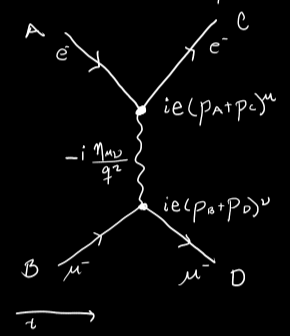
\includegraphics[width=6.5cm ]{2321.png}

El scattering entre un $e^-$ y un $\mu^-$  a orden \[
e^2
\] 

\begin{itemize}
    \item Por cada intercambio (propagador) de fotón \[ - \frac{\eta_{\mu \nu} }{q^2}\]
    \item  La conservación de energía y momento en el vértice. \[P=(E,P), \quad P^\mu P_\mu = E^2-P^2=m^2=P^2 \] .
\end{itemize}

\end{multicols}
\begin{itemize}
    \item $q^2 \not = 0$ en general, $q = P_D-P_B $, decimos que el fotón es virtual. 
    \item  Por cada vértice asociamos un término proporcional a $e$ y a la suma de los cuadrimomentos conectados al vértice. 
\end{itemize}
\end{minipage}

 

\begin{minipage}{0.9\textwidth}
\begin{multicols}{2}
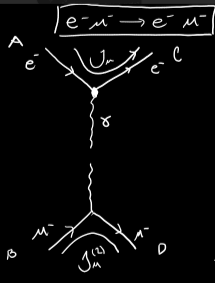
\includegraphics[width=6cm]{3321.png}

\begin{align*}
&-i \int d^4 x A^\mu \mathcal{J}_ \mu  \\
&\square A^\mu = \mathcal{j}^\mu _{(2)} \\
& T_{fi} = -i N_AN_BN_CN_D (2\pi )^4 \delta^4 (P_A+P_B-P_C-P_D ) \mu \\
& -i \mu = \underbrace{\qty[i e (P_A+P_C)^\mu ] }_{\texttt{vértices}} \underbrace{\qty(- \frac{i \eta_{\mu \nu}}{q^2})}_{\texttt{Propoagadores}} \underbrace{\qty[ie (P_B+P_D )^\nu]}_{\texttt{vértice}}
\end{align*}
\end{multicols}
\end{minipage}
\vspace{2ex}

$\to $ vértice  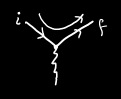
\includegraphics[width=2cm]{4321.png} \[ ie (P_i +P_f )^\mu  \]
 
 $\to $ Propagador:
\begin{tikzpicture}[remember picture, overlay]
  \feynmandiagram {
    a -- [photon] b,
  };
\end{tikzpicture}
\[
- \frac{i  \eta_{\mu \nu }}{q^2}
\]
$q:$ por conservación de energía-momento
  
\subsection{El origen del propagador}


\begin{align*}
\to T_{fi}^{(2)} &= -i \sum_{n\not =j} V_{fn} \frac{1}{E_i-E_n } V_{ni } 2 \pi \delta (E_f-E_i) \\
\text{ Cómo puedo pasar} \\
\frac{1}{E_i -E_n} &\to \frac{1}{(P_A+P_B)^2} \quad\Large\text{? }
\end{align*}

Consideremos $e^- e^+$ 

\begin{center}
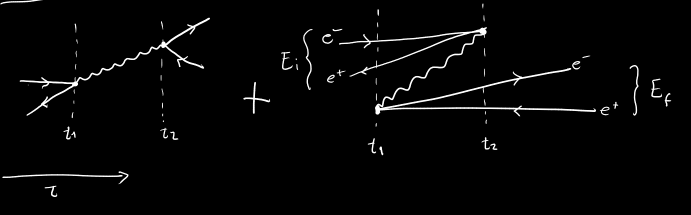
\includegraphics[width=13.5cm]{5321.png}
\end{center}
\begin{align*}
\mu &= V_{in} \frac{1}{E_i -E_ \gamma }V_{nf} + V_{in} \frac{1}{E_i-\underbrace{E_i+E_f+E_\gamma}_{2E_i +E_\gamma} } \\
\mu &= V_{in}  \qty(\frac{1}{E_i -E_\gamma } - \frac{1}{ E_i +E_\gamma } )V_{fn} \\
&= V_{in} \qty(\frac{E_i +E_f -E_i+E_\gamma }{E_i^2 -E_\gamma^2} ) V_{nf} = V_{in} \qty(\frac{2E_\gamma}{E_i^2-E_\gamma^2 } )V_{nf}
\end{align*}
$\Rightarrow $ La energía no se conserva, se conserva el momento.

$\Rightarrow$ Las partículas son físicas \( P^2 = m^2\)

\begin{align*}
    (E_i)^2 &= (P_i)^2+(\Vec{P}_i)^2= (P_A+P_B)^2+(\Vec{P}_A+\Vec{P}_B)^2 \\
    (E_\gamma) &= m \gamma^2 + (\Vec{P}_\gamma)^2, \quad \Vec{P}_\gamma = \Vec{P}_A +\Vec{P}_B \\
    \frac{1}{E_i^2 -E_\gamma} &= \frac{1}{(P_A+P_B)^2+(\Vec{P}_A +\Vec{P}_B )^2- m \gamma^2- (\Vec{P}\gamma )^2 } = \frac{1}{(P_A+P_B)^2-m \gamma^2 } \to \frac{1}{q^2}
\end{align*}

Para el proceso: \( \gamma e^- \to \gamma e^-\) \hspace{1cm} VS

\begin{minipage}{0.9\textwidth}
\begin{multicols}{2}
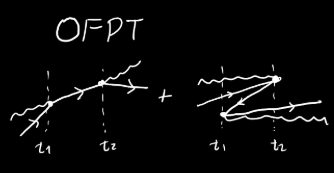
\includegraphics[width=6cm]{6321.png}

\begin{itemize}
    \item EL momento se conserva pero la energía no.
    \item  Las partículas  intermedias Están siempre en la capa de masas $( P^2 =m ^2)$. 
\end{itemize}
\newpage
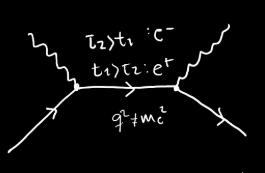
\includegraphics[width=6cm]{7321.png}


\begin{itemize}
    \item Los cuadrimomentos se conservan en el vértice. 
    \item La partícula intermedia no está en la capa de masas.
\end{itemize}
\end{multicols}


\end{minipage}


\subsection*{25 de marzo }

Se discute lo visto en la clase del 21 de marzo, para la interacción $\boxed{e^- \mu ^- \to e^- \mu^- }$. 
\subsection{ Scattering de Electrones}
\begin{minipage}{0.9\textwidth}
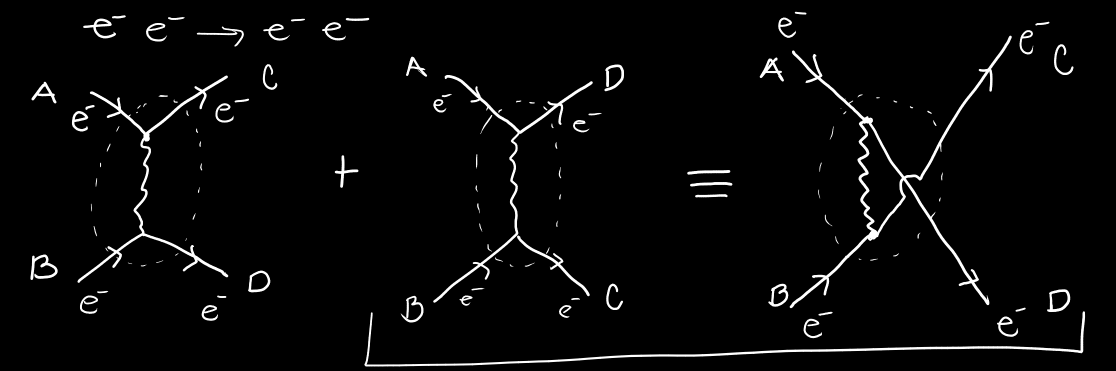
\includegraphics[width=0.90 \textwidth]{C2503/01.png}
\end{minipage}

\begin{align*}
    - \mu _{e^-e^- \to e^-e^-} &= ie (P_A +P_C )^\mu \frac{- i \eta_{\mu \nu } }{ (P_D-P_B)^2 }ie (P_B+P_D)^\nu \textbf{+} ie (P_A+P_D)^\mu  \frac{-i \eta_{ \mu \nu }}{(P_C-P_B)^2 } ie(P_B+P_C)^\nu 
\end{align*}

Notar que hay una simetría con respecto de $C\leftrightarrow D $, nos asegura una simetría $A\leftrightarrow B$. 

\[
-i \mu_{e^-e^- \to e^- e^-  } = -i \qty(-\frac{e^2(P_A+P_C)^\mu (P_B+P_D)_\mu  }{(P_D-P_B)^2  }  -\frac{e^2 (P_A +P_D )^\mu (P_B +P_C)_\mu  }{(P_C-P_B)^2 })
\]
\subsection{Scattering electrón- positrón  ($e^- e^+\to e^- e^+$)} 


\begin{center}
    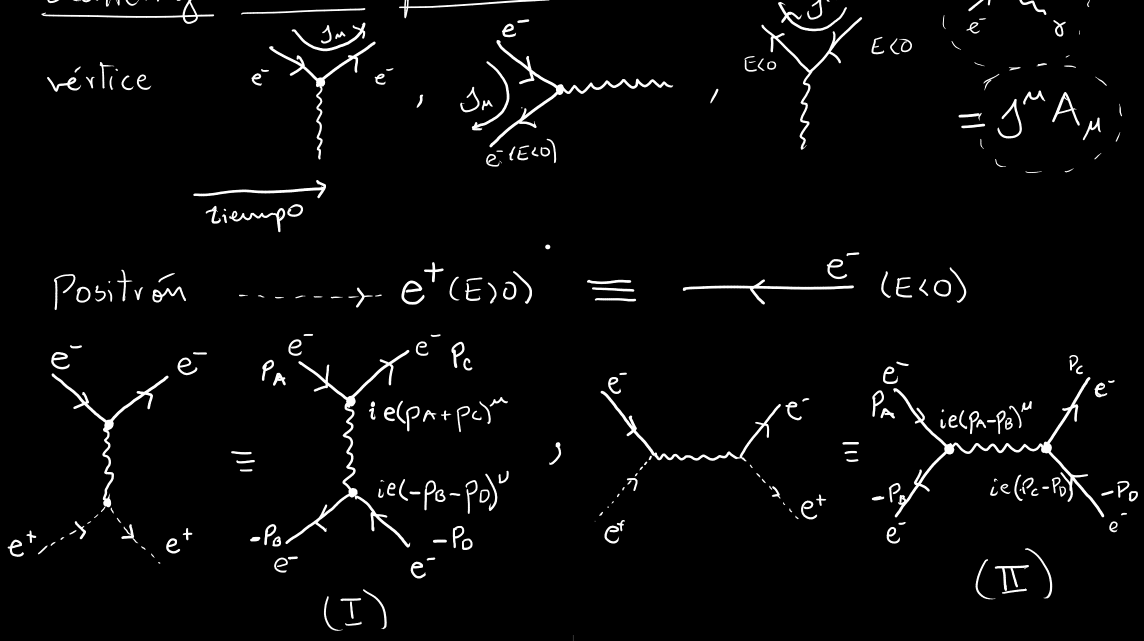
\includegraphics[width= 0.8\textwidth ]{C2503/02.png}
\end{center}
\[
-i \mu_{e^-e^+ \to e^-e^+} = -i \qty(\frac{-e(P_A +P_C )^\mu (-P_B-P_D)_\mu  }{(p_B-P_D)^2  } -\frac{e ^2(P_A -P_B)_\mu (P_C -P_D)^\mu   }{(P_C+P_D)^2 } )
\]
Simetría $P_C \leftrightarrow -P_B $
\begin{ejercicio}
    Verificar:
    \[
    \mu_{e^+ e^- \to e^+e^-} (P_A,P_B,P_C, P_D) = \mu_{ e^-e^- \to e^-e^-} (P_A, -P_D, P_C, -P_B)
    \]
\end{ejercicio}

\begin{tarea}
Usando las reglas de Feynmann para obtener la amplitud de los procesos:
\begin{itemize}
    \item $e^- \mu ^+ \to e^- \mu^+$ 
    \item  $e^+ e^- \to \mu^- \mu^+$
\end{itemize}
\end{tarea}

\subsection*{28 de marzo }
\subsection{Sección Eficaz }



Función de onda de la partícula libre 
\[
\phi = N e^{-i p \cdot x } 
\]
Recordemos que la densidad de probabilidad para partículas de espín 0
\[
\rho =2 E \abs{N}^2
\]
$\to $ El que sea proporciona a la energía compensa la contracción de volumen y nos deja el número total de partículas invarainte. 

Vamos a escoger la normalización para que existan  2E partículas por unidad de volumen $V$ 
\[
\int_V d V \rho = 2 E \to  N = \frac{1}{\sqrt{V} } 
\]

Para un proceso $A+B \to C+D$, calculamos la transición por unidad de tiempo y volumen.

\begin{center}
\begin{minipage}{0.85\textwidth}
\begin{multicols}{2}
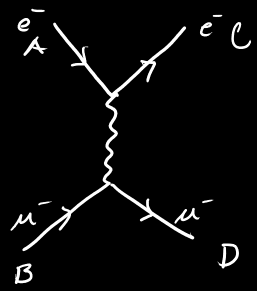
\includegraphics[width= 0.35 \textwidth]{C2503/283.png}


\[
W_{fi } = \frac{\abs{_{T_{fi}} }^2 }{TV}
\]

Donde 
\[
T_{fi} = - i N_AN_BN_CN_D (2 \pi)^4 \delta^4 (P_C+P_D-P_A-P_B) \mu 
\]
\end{multicols}
\end{minipage}
\end{center}


Al elevar al cuadrado $T_{fi}$ dejamos una de las deltas como la integral de una función exponencial. Al utilizar $\delta^4 (\sum P_i )$ para evaluar la función exponencial dando como resultado la integral de volumen y tiempo $(TV)$:

\begin{align*}
W_{fi} &= \frac{\frac{1}{V4 }(2\pi )^4 \delta^4 (P_C+P_D-P_A-P_B)(TV) \abs{\mu}^2  }{TV} \\
W_{fi} &= \frac{(2 \pi)^4 \delta^4 (P_C+P_D-P_A-P_B) \abs{\mu }^2  }{V^4}
\end{align*}

Sección eficaz $=\frac{W_{fi}}{\text{flujo inicial}} $ ( número de estados finales) 


Número de estados finales en un volumen V:

Primero, vamos mostrar que $dt dv$ es un invariante. Consideremos dos sistemas de referencia, uno en reposo $\mathcal{O}_x$ y otro que se mueve a velocidad $v, \mathcal{O}_y$ 
\[
y^\mu = \Lambda^\mu_{\hspace{2ex}   \nu}  x^\nu 
\]
Para pasar del diferencial de volumen $d^4 x$ hacemos un cambio de variable: 
\[
\int d^4 x \Rightarrow \int d^4 y \abs{ \frac{\partial y^\mu }{ \partial x^\alpha }}, \quad \frac{\partial y^\mu }{\partial x ^\alpha } = \Lambda ^\mu_{\hspace{2ex} \nu } \frac{ \partial x^\nu }{\partial x^\alpha  } = \Lambda ^\mu _{\hspace{2ex} \alpha }
\]
El  jacobiano es el determinante de $\Lambda $, que sabemos para las transformaciones de lorentz propias y homogéneas = 1. 

\begin{ejercicio}
4.1 de Halzen: 

Para un volumen $V = L ^3$ mostrar que el número de estados de momento permitidos en un rango $P_x, P_x+dP_x$ es $\frac{L}{2\pi } dP_x$ 
\end{ejercicio}

Número de estados finales/partícula =$\frac{V d^3 P}{(2\pi )^3 2E  }$ 


Número de estados finales = $\frac{V d^3 P_c}{(2\pi)^3 2E_c }\frac{ Vd^3 P_D}{(2\pi )^3 2E_D} $


Respecto al flujo inicial, en el sistema de referencia del laboratorio: 
Número de partículas atravesando una unidad de área por unidad de tiempo: 
\[
\abs{\vec V _A} \frac{2E_A}{V} 
\]

 Por lo que el flujo inicial $= \abs{\vec V_A } \frac{ 2E_A}{V}\frac{2 E_B}{V} $ 

Al sustituir los factores de volumen se cancelan: 
\[
d\sigma = \frac{ \abs{ \mu  }^2 }{F } d Q
\]
¿ Esto es invariante Lorentz ? 
\begin{align*}
    \to& \underbrace{ \int d^4 P}_{\texttt{invariante} } \delta \underbrace{ (P_0^2 - \vec P ^2-m ^2 )}_{\texttt{invariante }} \Big|_{P_0 > 0} = \int d^3 \vec P\frac{ 1}{2E } \\
    \to& F = \abs{\vec A} 2 E_A \cdot 2E_B \quad \text{ si } \quad \abs{\vec V_a} = \vec P_A/E_A\\
    & F= \abs{\vec V_A-\vec V_B  } \cdot 2E_A \cdot 2E_B \\
    & = 4(\abs{P_A}E_B  -\abs{P_B}E_A  ) = \dots = 4\qty[(P_A-P_B)^2- m_A^2m_B^2  ]^{1/2}
\end{align*}
\subsection{La ecuación de Pauli} 

\[
\underbrace{\frac{1}{2m } \vec P^2 \psi = E \psi}_{\text{partícula libre}} \to \begin{cases}
    \vec P \to \vec P +e \vec A \\
    P^0 \to P^0+e \phi 
\end{cases}\to \underbrace{\frac{1}{2m }(\vec P+e \vec A )^2\psi = E \psi   }_{\text{No término de espín }} \Big|_{\phi =0}
\]

Ecuación de Pauli $\{\frac{1}{2m}  (\vec P + e\vec A )^2 + \frac{e}{2m} \vec S \cdot \vec B \}\psi = E \psi  $

Pero $\psi = \phi(x) \mathcal{X}$ 


El término 
\[
(\vec P +e \vec A  )^2 \psi \to \qty (-\frac{\nabla^2 \psi  }{2m }+ \underbrace{ \frac{e}{2m} \vec B \cdot \vec L }_{\text{E potencial }}+\frac{e^2}{2m^2} A^2 )\psi 
\]
\[
\vec M = -\frac{e }{2m } \vec L 
\]
De forma análoga puedo proponer que la energía a autovalores $\pm \frac{1}{2}$ de $S_z$. 

Para $\vec B = (0,0,B)$ 
\[
\frac{e B}{2m } S_z \quad \text{donde} \quad [S_i, S_j] = i \epsilon_{ijk}S_k
\]
Pero el valor observado e el doble para autovalores $\pm \frac{1}{2}$ de $S_z$ 
\begin{align*}
    \frac{g e B}{2m} S_z \hspace{4ex} g&: \text{ Razón giromagnética del electrón }  \\
    g &\approx  2
\end{align*}
Uno de los triunfos de la ecuación de Dirac es predecir $g =2$ . El término asociado al espín:
\[
\qty( \frac{e}{ 2m}\vec \sigma \cdot \vec B  ) \psi  \quad \psi = \phi(x )\chi
\]
La ecuación de DIrac: 

$\to $ En el límite no relativista $\psi = u(p) e^{-i P\cdot x}$ 

\begin{align*}
    H u &= (\vec \alpha \cdot \vec P + \beta m) u = Eu \\
    &= \begin{pmatrix}
        m & \vec \sigma \cdot \vec P\\ \vec \sigma \cdot \vec P &-m
    \end{pmatrix} \begin{pmatrix}
        u_A \\u_B
    \end{pmatrix} =E\begin{pmatrix}
        u_A \\u_B
    \end{pmatrix}
\end{align*}
que se puede reescribir como: 
\begin{align*}
    \vec \sigma \cdot \vec P u_B &= (E-m) u_A \\
    \vec \sigma \cdot \vec P u_A&= (E+m) u_B
\end{align*}
Cimparemos el tamañano de los espinores: 
\begin{align*}
    (\vec \sigma \cdot \vec P  )^2 \abs{u_B }^2 &= ( E-m)^2 \abs{u_A}^2 \\
    \frac{\abs{u_B}^2 }{\abs{u_A}^2  } &= \frac{ (E-m)^2 }{P^2 }\xrightarrow{N.R.} \frac{ (m+\frac{P^2}{2m }-m )^2 }{P^2} = \frac{P^2}{4m^2} = \frac{v }{4}
\end{align*}


\section{1 de abril }
\subsubsection{Ecuación de dirac }
En el límite no- relativista de la ecuación de Dirac 
\[
\psi = \begin{pmatrix}
    \psi_A \\ \psi_B 
\end{pmatrix}, \quad \frac{\abs{\psi_A}}{ \abs{\psi_B} } \propto \frac{c}{v}
\]

 La ecuación de Dirac $P'$ partícula cargada en presencia $A^\mu $
\[
P^\mu \Rightarrow P^\mu +e A^\mu 
\]
\begin{align*}
    \begin{pmatrix}
        \mathbb{I}_{2\times 2} m & \sigma\cdot (\vec P +e \vec A ) \\\sigma\cdot (\vec P +e \vec A ) & -m \mathbb{I} _{2\times 2} 
    \end{pmatrix}\begin{pmatrix}
        \psi_A\\\psi _B
    \end{pmatrix} &= (E+e A^0) \begin{pmatrix}
        \psi_A \\\psi_B
    \end{pmatrix} \\
    (m-e A^0) \psi_A +\sigma\cdot (\vec P +e \vec A )\psi_B &= E \psi_A \\
    \sigma\cdot (\vec P +e \vec A )-(m+e A^0) \psi_B&= E \psi_B \quad \leftarrow
\end{align*}
En el límite No relativista $m \gg e A^0$ , m $ m \gg E_{\rm Kin}^{\rm NR} $, $E = m +E_{\rm Kin}^{\rm NR}$

\begin{align*}
\sigma\cdot (\vec P +e \vec A ) \psi_A &= \underbrace{ (E+m+eA^0)\psi _B }_{m+2E_{\rm Kin }^{NR}  =2m} \\
\psi_B &= \frac{\sigma\cdot (\vec P +e \vec A ) }{ 2m }\psi_A
\end{align*}
Sustituyendo: 
\[
\boxed{[\sigma\cdot (\vec P +e \vec A )] [\sigma\cdot (\vec P +e \vec A )]\psi_A =2m (E-m eA^0 )\psi_A   }
\]



\begin{align*}
[\sigma\cdot (\vec P +e \vec A )][\sigma\cdot (\vec P +e \vec A )]&= ( \vec \sigma\cdot \vec P)( \vec \sigma\cdot \vec P)+ e(\sigma\cdot \vec P)( \vec \sigma\cdot \vec A) +e(   \sigma\cdot \vec A)( \vec \sigma\cdot \vec P) +e^2( \vec \sigma\cdot \vec A)( \vec \sigma\cdot \vec A) \\
\text{Pero} \\
( \vec \sigma\cdot \vec P)( \vec \sigma\cdot \vec P)&= P^2\\
&= \vec P^2 +e^2 \vec A^2+e [( \vec \sigma\cdot \vec P)( \vec \sigma\cdot \vec A) +( \vec \sigma\cdot \vec A) ( \vec \sigma\cdot \vec P)  ] 
\end{align*}
Tomando solo el último término:
\begin{align*}
( \vec \sigma\cdot \vec P)( \vec \sigma\cdot \vec A) +( \vec \sigma\cdot \vec A)( \vec \sigma\cdot \vec P) &= \sigma^i P^i\sigma^j A^j+\sigma^i A^i\sigma^j P^j \quad ij =1,2,3 \\
&= \mathbb{I} \vec P \cdot A+ \mathbb{I} \vec A \cdot \vec P  + \sigma^i\sigma^j(P^i A ^j+A^i P^j)_{i \not =j}\\
\sigma^i\sigma^jP^iA^j+\sigma^j\sigma^i P^j A^i &= i \epsilon^{ijk} \sigma^k (P ^iA^j-P^j A^i )_{i<j}\\
&= i \sigma^k [\epsilon^{ijk} (P^i A^j-P^j A^i) ]_{i<j} \\
&= i\sigma \cdot (\vec P \times \vec A) \\
\sigma^i\sigma^j A^jP^i\Big |_{i \not = j}&=i \sigma\cdot (\vec A\times \vec P)
\end{align*}

\begin{align*}
    \sigma^iP ^i\sigma^jA^j&=\underbrace{i \epsilon_{ijk} P^iA^j}_{(P\times A)_k } \sigma_k
\end{align*}
\begin{tarea}
    Mostrar que: 
    \[
    (\vec P \times \vec A  +\vec A \times \vec P ) \psi = -i \nabla \times A \psi = -i B \psi 
    \]
\end{tarea}

Sustituyendo
\[
i \sigma \cdot (\vec P \times \vec A  + A \times \vec P ) \psi = \vec \sigma \cdot \vec B
\]
Uniendo todas las partes: 
\[
[\sigma \cdot  (\vec P +\vec A) ] [\sigma\cdot (\vec P + \vec A  )]= (\vec P +e \vec A )^2 +e\vec \sigma \cdot \vec B
\]
\subsubsection{El límite no relativista de la ecuación de dirac.}
   \[
   P^\mu \to P ^\mu +e A^\mu
   \]
\[
[\sigma (\vec P + \vec A)][\sigma\cdot (\vec P +\vec A ) ] = (\vec P +e \vec A )^2 +e \vec \sigma\cdot \vec B
\]
Sustituyendo
\[
\{  (P +e\vec A )^2+e \vec \sigma \cdot \vec B\} \psi _A= \underbrace{(E+m )}_{2m}(E-m +e A ^0) \psi_A 
\]
No relativista: 
\[
E =m +E_{\rm Kin}^{\rm NR}, \quad m \gg E_{\rm Kin}^{\rm NR}, \quad m \gg e A^0
\]
Sustituyendo: 
\[
\{ (P+e\vec A)^2+e\vec \sigma \cdot \vec B\} \psi _A= 2m (E_{\rm Kin}^{NR}+eA^0 )\psi_A\Big|\psi= \phi (x) \chi 
\]
\[
\qty[\frac{1}{2m} (P+e\vec A)^2+ \frac{e}{2m } \vec \psi \cdot \vec B -e A^0] \psi_A = E_{\rm Kin }^{\rm NR} \psi_A .
\]
$\psi$ no es una función escalara, lo debo de escribir como :
\[
\psi = \phi(x) \chi 
\]
 

\[
\vec \mu  = -\frac{e}{2m}\vec L.
\]


Resultado muy importanta: 

\[
\vec \mu = -\frac{e}{m} \vec \sigma= -g \frac{e}{2m}\vec S
\]
Donde \[
g=2.
\]

Esta es la razón giro-magnética del electrón. 
El valor experimental es $g=2.000232$

\begin{center}
\begin{minipage}{0.85\textwidth}
\begin{multicols}{2}
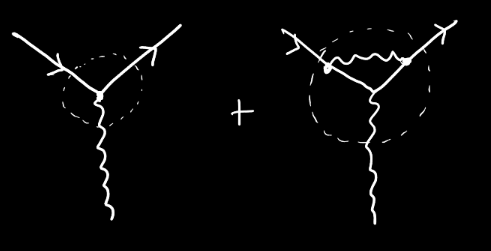
\includegraphics[width=0.5 \textwidth]{C2503/014.png}


\[
g = 2 + \frac{\alpha}{\pi }
\]
Hasta orden $\alpha^3$
\[
\qty( \frac{g-2}{2})  =(1159655.4\pm 3.3)\times10^{-9}
\]
\[
\qty(\frac{g-2}{2} )_{\rm exp} =(1159657 \pm 3.5) \times 10^{-9}
\]

\end{multicols}
\end{minipage}
\end{center}

\begin{ejercicioimportante}
Ejercicio 8.4 de Aitchison
\begin{center}
 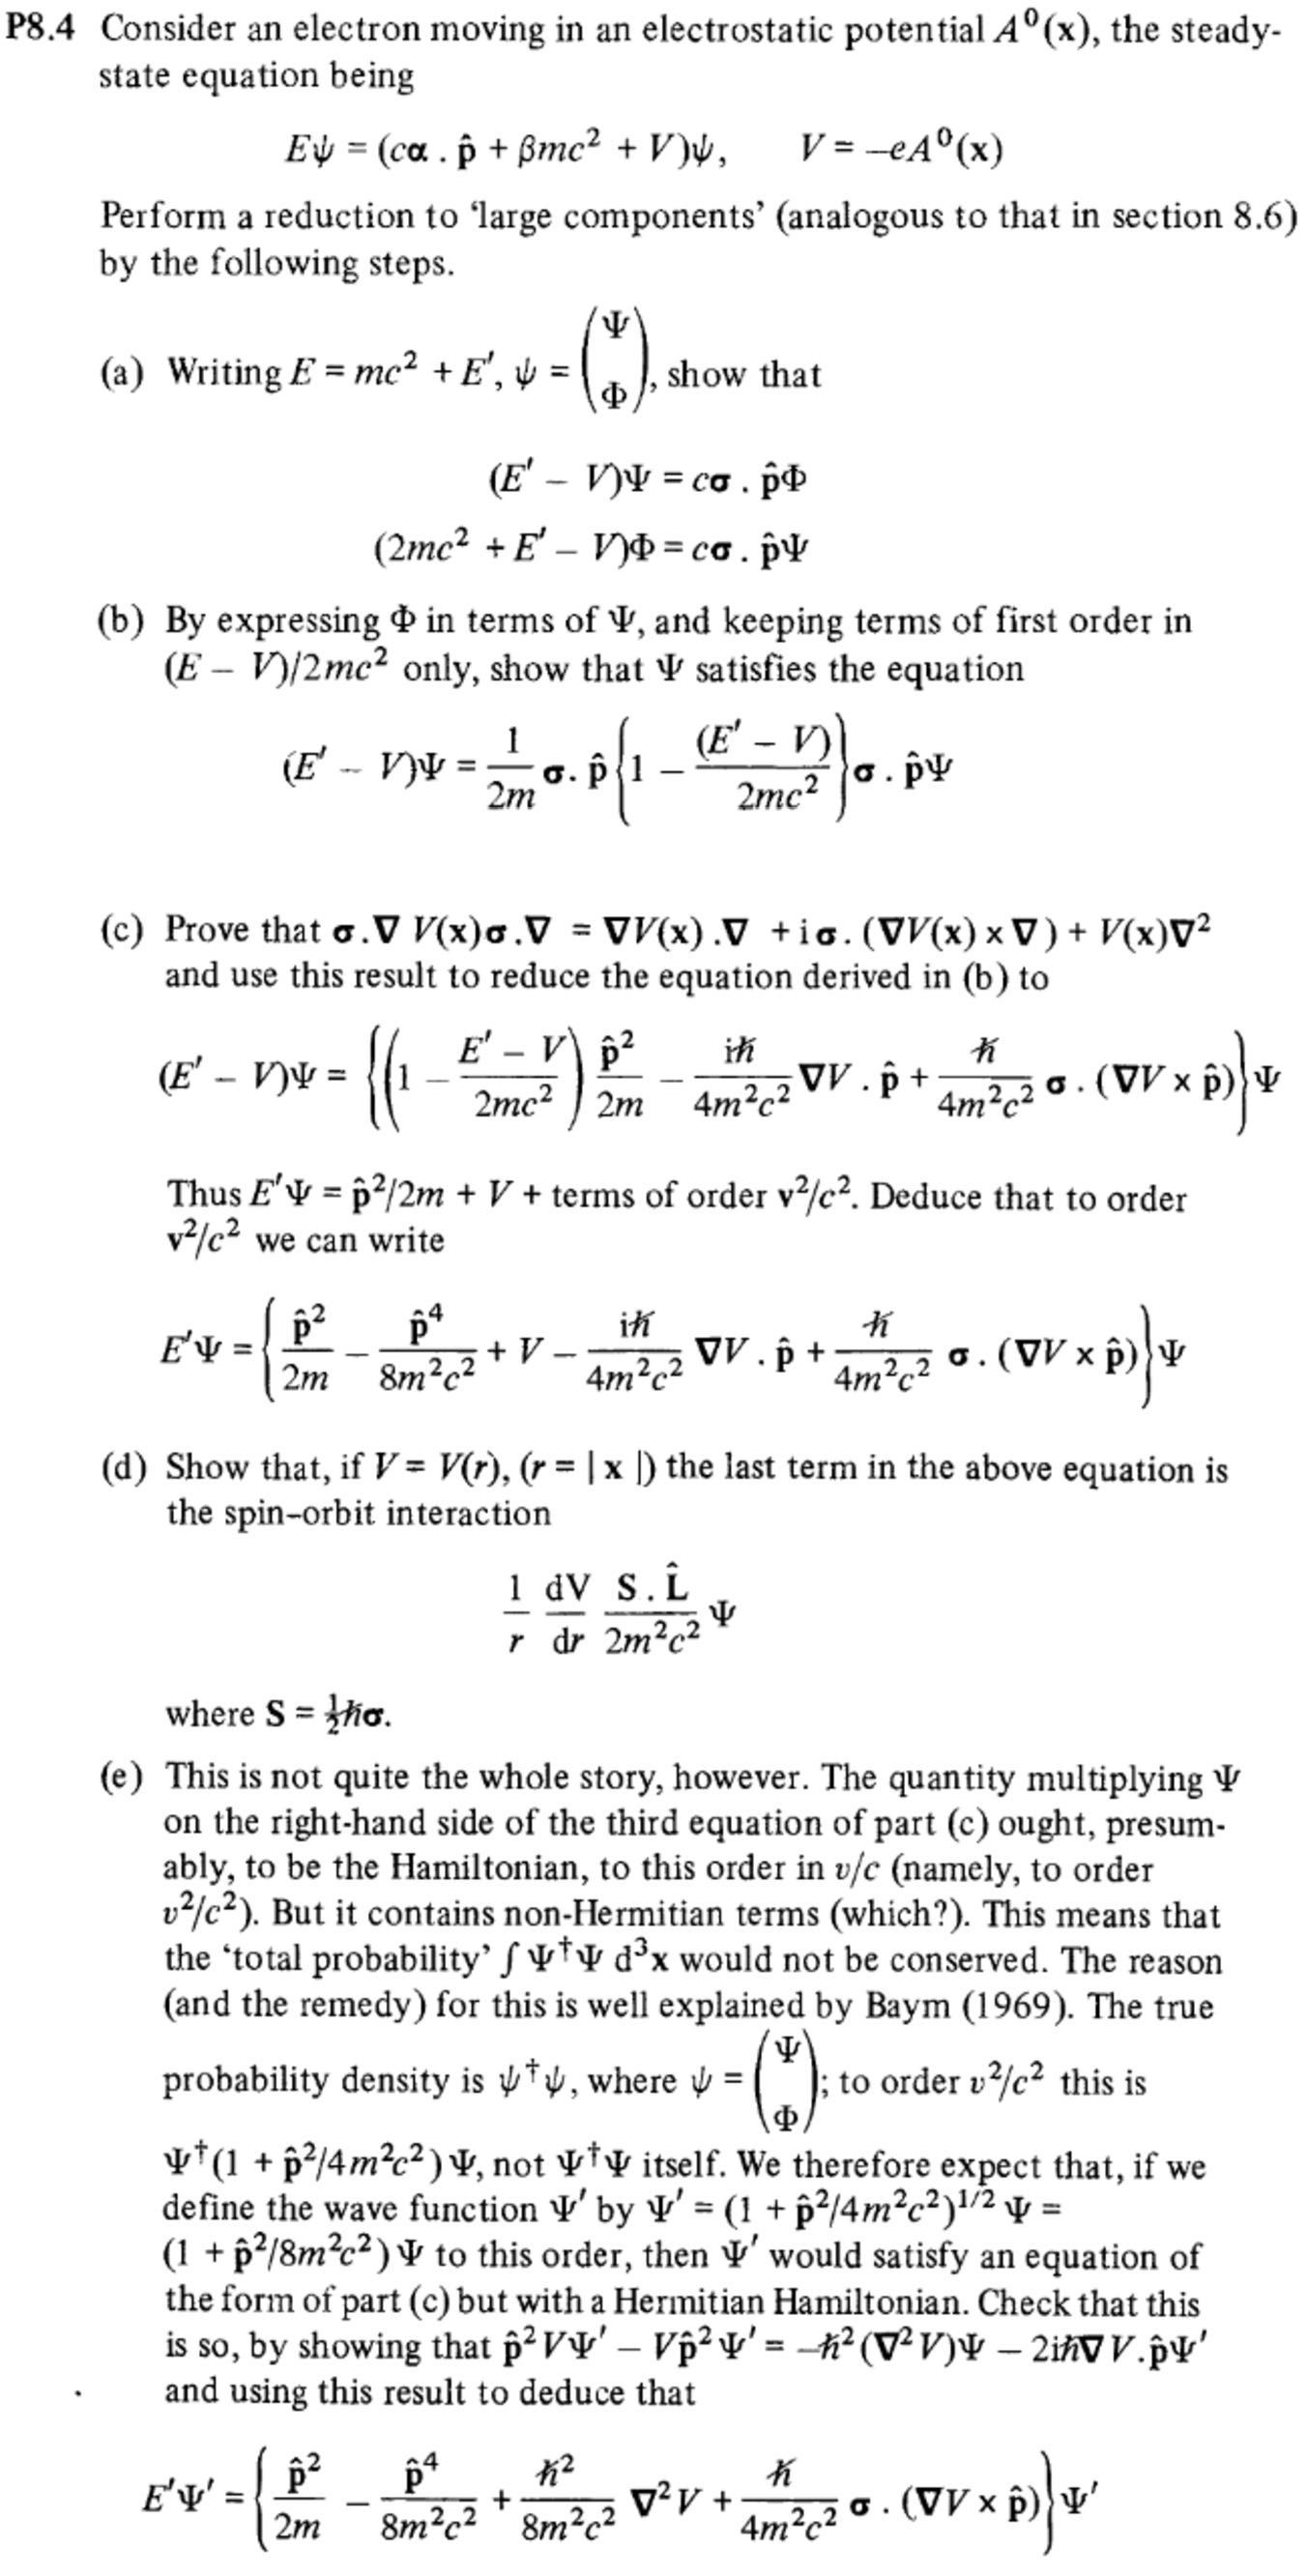
\includegraphics[width=0.7\textwidth ]{Aitchison_ejercicio-8.4.pdf}   
\end{center}
 
\end{ejercicioimportante}
La ecuación de Dirac para $u(\vec p)$ $\not A = \gamma^\mu A_\mu$
\[
\boxed{(\not P -m  )u(\vec p  ) =0 }
\]

Para $v(\vec p)$ 
\begin{align*}
    (-\not P -m ) u(-\vec p) &=0\\
    (\not P +m) v (\vec p) &=0, \quad P^0= E>0
\end{align*}
\subsubsection{Operador de carga}
\[
[\gamma^\mu (i \partial_\mu +e A_\mu   )- m ] \psi =0 \quad \checkmark
\]
Debe de debería poder escribir la ecuación de Dirac, para positrnes: 
\[
[ \gamma^\mu(i \partial_\mu -e A_\mu    )- m  ]\psi_c =0 \quad \leftarrow \quad \checkmark
\]
Necesitamos encontrar una transformación que cambie de signo el término proporcional a $e$.
\begin{align*}
\qty([\gamma^\mu (i \partial_\mu +e A_\mu  )-m ]\psi  ) ^* &=0 \\
[(-)\gamma^{\mu *  }( i \partial_\mu-eA_\mu ) -m ]\psi^*&=0
\end{align*}

Un operador que satisfaga
\begin{align*}
    \Rightarrow \quad - (C \gamma^0 ) \gamma^{\mu *}  = \gamma^\mu (c \gamma ^0)\hspace{5ex} \psi_c &= C\gamma^0\psi^* = c(\psi^\dagger\gamma^0)^T \\
    \psi_c&= C \overline{ \psi} ^T.
\end{align*}
\[
O [ -\gamma^{\mu * } ( i \partial_\mu-e A_\mu) -m  ]\psi^*=0
\]
 
\[
\begin{array}{cc}
   -\text{O} \gamma^{\mu  *}= \gamma^\mu\text{O}    &  - m \underbrace{ \text{O}\psi^* }_{\psi_c}  =0, \quad \psi_c= \text{O} \psi^*
\end{array}
\]
\[
\gamma ^\mu \quad (i \partial_\mu -eA_\mu ) \underbrace{\text{O} \psi^*}_{\psi_c}=0
\]
\begin{tarea}
    En la representación de Pauli-Dirac. Mostrar que una opción para $C$ es: 
    \[
    C\gamma^0 = i \gamma^2= \begin{pmatrix}
        0&0&0&1\\0&0&-1&0\\0&-1&0&0\\1&0&0&0
    \end{pmatrix}
    \]
\end{tarea}
\begin{ejercicio}
    \begin{align*}
        C^{-1} \gamma^\mu C &= (-\gamma^\mu)^T \\
        C &= -C^{-1} =-C^\dagger= -C^T \\
        \overline{\psi}_c&= - \psi^TC^{-1}
    \end{align*}
\end{ejercicio}


\subsection{4 de abril }
\subsubsection{Antipartículas }

\[
\mathcal{U}^{(1,2)} e^{-i px} \quad \text{ Electrones, con } E>0
\]
recordemos la interpretación de Feynamnnn - Stückelberg. 
\[
\begin{array}{c| |c}
     \texttt{Ecuación K-G  }&  e^-: E, \vec P \to \mathcal{J}^\mu (e^-)=2e \abs{N}^2(E, \vec P)    \\
     \mathcal{J}^\mu =-ie (\phi^* \partial^\mu \phi -\phi \gamma^\mu \phi^*  ) & \texttt{ Positrón} \\
     = -2e \mathcal{P}^\mu & e^+: \vec E, \vec P \to \mathcal{J}^\mu(e^+) = 2e \abs{N}^2(\vec E,  \vec P  )\\
     & =-2e\abs{N}^2 (-\vec E, -\vec P)
\end{array}
\]
\[
\mathcal{U}^{(3,4 )}  (-\vec P)e^{-i (-P)x } \equiv \mathcal{V}^{2,2 } e^{+ i Px }.
\]

Para $\mathcal{V}^{1,2} $, $P^0=E>0$ 

La ecuación de Dirac para $u(p)$  $\not A = \gamma ^\mu A_\mu$ 
\[
(\not P-m) u(\vec P)=0
\]
para $v(\vec p)$ 
\begin{align*}
(-\not P-m ) u(-\vec P ) &=0 \\
(\not P + m) v(\vec P)&=0. \quad P^0=E>0
\end{align*}
\subsubsection{Covarianza}
$\to$ Para la ecuación de Schrödinger sea covariante: $\phi'(x') =  \phi(x)$.
\[
\psi(x) = \phi(x) \mathcal{X}_{1/2}
\]
Entonces
\[
\phi'(\vec r) = \phi (R^{-1} \vec r) . \quad \vec r' =R \vec r
\]
\begin{align*}
\phi' &= u \phi  \\
u\phi (x,y,z)&= \phi ( \underbrace{R^{-1} \vec r }_{r'}\approx \phi (x+\epsilon y, y - \epsilon x, z), \quad \epsilon \ll 1
\end{align*}
Expansión para $\phi$ en términos de $\epsilon $.
\begin{align*}
&\approx \phi(x,y,z) + \epsilon \qty(\frac{\partial \phi }{\partial x } y - \frac{\partial\phi }{\partial y }  x) \\
&= \qty(1- i \epsilon \underbrace{(xP_y -y P_x )}_{\texttt{ Momento angular en z}} ) \phi (x)\quad \checkmark \\
\mathcal{U} \phi(x,y,z) &= (1-i \epsilon J_3 ) \phi \quad e^{i\theta _a T_a } \quad SO(3)
\end{align*}
Puedo identificar el generador $J_3 $ de las rotaciones. Con el operador momento angular. 
\[
\phi ^a (x) \to D [\Lambda ]^a _{\hspace{2ex}b  } \phi^b(\Lambda ^{-1} x) 
\]
$D[\Lambda ]:$ Elemto de una representación del grupo de lorentz. 

$\to $ Introducimos las álgeras de Clifford: 
\[
\{ \gamma^\mu, \gamma^\nu \} = \gamma ^\mu \gamma^\nu + \gamma ^\nu \gamma^\mu =2 \eta^{\mu \nu }, \quad \mu  =0,1,2,3
\]
\[
S^{\rho \sigma } = \frac{1}{4} [\gamma^\rho, \gamma ^\sigma ] = \begin{cases}
    0 \quad \rho =0 \\
    \frac{1}{2} \gamma^\rho \gamma ^\sigma \quad \sigma \not = \rho 
\end{cases} = \frac{1}{2} \gamma^\rho \gamma^\sigma- \frac{1}{2} \eta^{\rho \sigma }
\]
Los generadores del grupo de Lorentz: 
\[
(\mu^{\rho \sigma} ) ^{\mu \nu } = \eta^{\rho \mu } \eta^{\sigma \nu } - \eta^{\rho \nu} \eta^{\sigma \mu } \quad \checkmark
\]
Se puede verificar: 
\begin{align*}
    [S^{\mu \nu }, \gamma^\rho ] &= \gamma^\mu \eta^{\nu \rho }  - \gamma^\nu \eta^{\rho \mu } \\
    [S^{\mu\nu}, S^{\rho \sigma} ]  &= S^{\mu \sigma }-S^{\nu \sigma }- S^{\nu \sigma } \eta^{\rho \mu} + S^{\rho \mu } \eta^{\nu \sigma}-S^{\rho \nu  }  \eta^{\sigma \mu }
\end{align*}

Los objetos sobre los que actúa las matrices $(S^{ \mu \nu})^\alpha_{\hspace{2ex} \beta } $ Son los espinores de Dirac. 
\[
\psi^\alpha(x) = S[\Lambda ]^\alpha_{ \hspace{2ex }\beta  }\psi ^\beta(\Lambda ^{-1}) 
\]
\begin{align*}
 \Lambda &= \text{ exp} \qty(\frac{1}{2}\Omega_{\rho \sigma } \mu^{\rho \sigma}  ) \\
 S(\Lambda ) &= \text{exp}  \qty(\frac{1}{2}\Omega_{\rho \sigma}S^{\rho \sigma}   )
\end{align*}
\subsection{25 de abril }
Recapitulación de Covarianza.


Puedo desmostar que $S^{\rho \sigma  }$ tiene la misma álgebra de Lie que  los generadores del Grupo de lorentez. 


Rotaciones:  $\rho, \sigma =i,j $ con $i,j =1,2,3$
\[
S^{ij } = \frac{1}{2} \begin{pmatrix}
    0& \sigma^i \\-\sigma^i &0 
\end{pmatrix} \begin{pmatrix}
    0& \sigma^j\\-\sigma^j &0 
\end{pmatrix} = -\frac{1}{2} \begin{pmatrix}
    \sigma^i\sigma^j&0 \\0&\sigma^i\sigma^j 
\end{pmatrix} =- \frac{i}{2} \epsilon^{ijk} \begin{pmatrix}
    \sigma^k&0\\0&\sigma^k
\end{pmatrix}
\]

Representación de weyl  

\begin{align*}
    \Omega_{ij} &= -\epsilon_{ijk }\theta^k \to \Omega_{12} = -\theta^3 \\
    \epsilon_{ijk} \theta^k\epsilon^{ijl} \sigma^l &= \delta^l_{\hspace{2ex } k} \theta^k \sigma^l = \vec \theta \cdot \vec \sigma \\
    S[ \Lambda ] &= \text{ exp} \qty(\frac{1}{2}\Omega_{\rho \sigma}S^{\rho \sigma}    ) \xrightarrow[\texttt{ rot}]{} \begin{pmatrix}
        e^{i\frac{\vec \theta \cdot \vec \sigma }{2}} &\vdots& 0 \\\dots &.& \dots \\0 &\vdots & e ^{i\frac{\vec \theta \cdot \vec \sigma }{2}}
    \end{pmatrix} \begin{pmatrix}
        \psi_L \\\dots \\\psi_R
    \end{pmatrix}
\end{align*}
$\texttt{ Rot} 2 \pi$ al rededor de $z$ .

\[
\Omega_{12} =-\Omega_{21} =- \theta_z \quad \vec \theta =(0,0, 2\pi )
\]

\begin{align*}
S[\Lambda] &= \begin{pmatrix}
    e^{i \pi \sigma^3 } &0\\0&e^{i \pi \sigma^3} 
\end{pmatrix} =    -\mathbb{I} \quad \begin{pmatrix}
    e^{i \pi}&&&\\&e^{-i \pi}&&\\&&e^{-i \pi}&\\&&&e^{-i \pi}
\end{pmatrix}\\
\psi^\alpha(x) &\to \psi^\alpha (x) 
\end{align*} 

Para un boost: 
\begin{align*}
S^{oi } &= \frac{1}{2} \begin{pmatrix}
    0&1\\1&0
\end{pmatrix} \begin{pmatrix}
    0&\sigma^i\\-\sigma^i&0
\end{pmatrix}= \frac{1}{2} \begin{pmatrix}
    -\sigma^i &\vdots &0\\\dots &. &\dots \\0& \vdots & \sigma^i
\end{pmatrix} \\
\Omega_{o i} &= - \Omega_{ i o} = \beta_i  \\
S[\Lambda ] &= \begin{pmatrix}
    e^{i\beta \sigma/2} &\vdots  &0 \\\dots& . &\dots \\0 &\vdots  & e^{- \vec \beta\cdot \vec \sigma/2}
\end{pmatrix}
\end{align*}

$\to $ Las representaciónes del generador de Lorentz no son unitarias: 
\[
S[\Lambda ]^{-1} = S [- \Lambda ]^\dagger \hspace{5ex} (S^{\rho \sigma}) ^\dagger=-S^{ \rho \sigma } \leftarrow \quad S[\Lambda ]^\dagger S[\Lambda ] = \mathbb{I} 
\]
\begin{align*}
\qty(\mathbb{ I}  + \frac{1}{2}\Omega_{\rho \sigma }   S^{\rho \sigma })^\dagger   \qty(  \mathbb{1} +\frac{1}{2} \Omega_{\mu \nu } S^{\mu \nu } )&=\mathbb{I} \\
1+\frac{1}{2} \Omega_{\rho \sigma} S^{\rho \sigma \dagger}  + \frac{1}{2} \Omega_{ \mu \nu }S^{\mu \nu }&= \mathbb{I }
\end{align*}
\begin{align*}
    S^{\mu \nu }&= \frac{1}{4} [\gamma^\mu, \gamma^\nu ] \\
    (S^{\mu \nu })^\dagger &= \frac{1}{4} \qty[( \gamma^\nu )^\dagger, (\gamma^\mu) ^\dagger  ] \\
    &= \frac{1}{4} \qty(\gamma^{\nu \dagger }\gamma^{\mu \dagger}- \gamma^{\mu \dagger}\gamma^{\nu \dagger}     ) \\
    &= - \gamma^0\qty(\frac{1}{4}[\gamma^\mu, \gamma^\nu ]    ) \gamma^0
\end{align*}
Recordemos $\gamma^0 \gamma^\mu \gamma^0=\gamma^{\mu \dagger} $, $(\gamma^0)^2=\mathbb{I}  $ \[
=- \gamma^0 S^{\mu \nu } \gamma^0 
\]
\[
\gamma^0(S^{\mu \nu } )^{-1} \gamma^0 
\]
\begin{align*}
\psi(x) &= \mathbb{I} + \frac{1}{2} \Omega _{ \rho \sigma} (S^{\rho \sigma}) ^{-1} \quad (S^{\rho \sigma -1 })^2\\
\psi^\dagger(x) &= \psi ^\dagger (\Lambda^{-1}x)   S[\Lambda]^\dagger\\
\psi^{'\dagger} \psi ' &= \psi^\dagger (\Lambda^{-1} x) S [  \Lambda ] ^\dagger S[\Lambda  ]\psi (\Lambda^{-1}x )+\psi^\dagger(x) \psi(x)\\
    S^{-1}&= \mathbb{I} +\frac{1}{2}\Omega_{\rho \sigma} (S^{ \rho \sigma })^{-1} \\
S[\Lambda ]^\dagger&= \gamma^0 (S[\Lambda]^{-1} ) \gamma^0
\end{align*}

\begin{align*}
    \overline{\psi} \psi = \psi^\dagger \gamma^0\psi \to & \psi^\dagger S[ \Lambda ] ^\dagger\gamma^0S[\Lambda ] \psi \\
    &\psi^\dagger \gamma^0 ( S[\Lambda ]^{-1} )\underbrace{\gamma^0\gamma^0}_{\mathbb{I}} S[\Lambda ] \psi \\
    &  \psi^\dagger \gamma^0\psi \\ 
    &= \overline{\psi} \psi 
\end{align*}

\subsubsection{Complemento de la clase:} 

$\to  \overline{\psi }\gamma^\mu \psi '= \overline{\psi}S[\Lambda ] ^{-1 }\gamma^\mu S[\Lambda ] \psi   $  

Qué esperaríamos:
\[
S[\Lambda] ^{-1} \gamma^\mu S[\Lambda] = \Lambda^\mu_{\hspace{2ex}\nu } \gamma^\nu 
\]

\begin{align*}
    \overline{\psi} ' \gamma^\mu \psi ' &= \Lambda^\mu_{ \hspace{2ex}\nu  } \overline{\psi} \gamma^\nu \psi \\
    \mathcal{J}'^\mu&= \Lambda^\mu_{\hspace{2ex}\nu  } \mathcal{J} ^\nu
\end{align*}
Transformación infinitesimal: 
\begin{align*}
\Lambda &= \text{ exp} \qty[ \frac{1}{2}\Omega_{\sigma\rho   }\mu^{\sigma \rho }   ] \approx \mathbb{I}+ \frac{1}{2} \Omega_{\sigma\rho } \mu^{\sigma \rho }  \\
S[\Lambda]&= \text{exp} \qty[ \frac{1}{2}\Omega_{\sigma \rho }  S^{\sigma \rho } ] \approx \mathbb{I} +\frac{1}{2} \Omega _{\sigma \rho  } S^{\sigma
 \rho} 
\end{align*}





\subsection{2de mayo Paridad} 

\[
P: \quad x^0 \to x ^o \quad x^i \to -x^i
\]
la paridad es una transformación que no puede ser descrita de esta forama( no puedo describir infinitesimalmente alrededor de $\mathbb{I}$) . pero si regreso a las características de las transformaciones de lorentz: 
\[
\Lambda = \begin{pmatrix}
    1&0&0&0\\0&-1&0&0\\0&0&-1&0\\ 0&0&0&-1\\
\end{pmatrix}
\]
Bajo transformaciones de paridad puedo mostrar que mi espinor: 
$\psi \to \gamma^0 \psi$.  


¿Cómo transforman los bilineales ? 
$\overline{\psi}\psi  \to $  $\overline{\psi }\psi $  escalar:

 

Veamos cómo transforma ahora: 

\[
\mathcal{J}^\mu = \overline{\psi } \gamma^\mu \psi  \to  
\begin{cases}
    (\overline{\psi} \gamma^0)\gamma^0 (\gamma^0 \psi) = \overline{\psi} \gamma^0 \psi  \\
        (\overline{\psi }\gamma^0 ) \gamma^i (\gamma ^0\psi) = - \overline{\psi } \gamma^i \psi 
\end{cases}  \quad \mathcal{J^\mu} ' = \Lambda ^\mu_{\hspace{2ex} \nu} \mathcal{J}^\nu 
\]

\subsection{Chiralidad } 
\[
\gamma^5 = i \gamma^0 \gamma^1\gamma^2 \gamma^ 3 
\]
\[
\{ \gamma^\mu , \gamma^5 \} =0 \quad (\gamma^5)^2 = \mathbb{I}  \quad [S^{\mu \nu  }, \gamma ^5 ] =0
\]
\[
P_{\pm} = \frac{1}{2} (1 \pm \gamma_5) \quad (P_\pm)^2 = P_\pm \quad P_+ P_- =0
\]

hay dos tipos de representaciones: pauli-dirac y la represntacion de weyl, la que hemos estado usando es la de pauli-dirac.

En la representación de weyl
\[
\gamma_5 = \begin{pmatrix}
    1&0\\0&-1
\end{pmatrix} \quad \psi_\pm  = P_\pm \psi \quad \psi = \psi_+ +\psi_-
\]

la representación no tuvo mucho exito porqué  los auto estados que representa no son autoestados físicos. 


 que pasa si en lugar de tener una matriz $\gamma$ tengo un $\gamma^5$? 

 \[
 \overline{\psi} \gamma^5\psi \Rightarrow P: \overline{\psi} \gamma^5 \psi \to \overline{\psi} \gamma^0 \gamma^5\gamma^0 \psi = - \overline{\psi} \gamma^5\psi
 \]
Esto transforma como un "pseudoescalar" 


que pasa si tengo: 
\[
\mathcal{F}^\mu   =  \overline{\psi}\gamma^5\gamma^\mu \psi \Rightarrow P: \overline{\psi} \gamma^5 \gamma^\mu \psi \to \overline{\psi} \gamma^0\gamma^5 \gamma^\mu  \gamma^0\psi= -\overline{\psi}\underbrace { \gamma^5\gamma^0\gamma^\mu \gamma^0}_{\gamma^{\mu \dagger}} \psi  
\]
\[
= \begin{cases}
    -\overline{\psi} \gamma ^5\gamma ^0 \psi \\
    \overline{\psi} \gamma^5\gamma^i \psi 
\end{cases} \quad i =1,2,3
\]

Esto representa como un vector axial. 


¿Cuál es la relevancia ? 

Lo que nos puede llamar la atención que el gamma 5 puede representar una proyección. 

Para entontrarle utilidad a esto, regresamos a 
\subsection{Fermiones sin masa}
Cuando escribimos la ecuación de dirac: 

\[
H \psi = (\overline{ \alpha}\cdot \Vec{P}+ \not\beta ^0m  ) \psi
\]
\[
\to \alpha_i \alpha_j+ \alpha_j \alpha_i =2 \delta_{ij} \hspace{2cm} \alpha_i^+ = \alpha_i 
\]
puedo escribir(puedo usar las matrices de pauli porque son de dimension par) : 

\begin{align*}
    E \mathcal{X} &= - \Vec{ \sigma }\cdot \Vec{P}  \mathcal{X} \quad \nu_{L}, 
 \overline{\nu }_R\tag{1}    \\
    E \phi &=  \Vec{ \sigma }\cdot \Vec{P} \phi\quad \nu_R, \overline{\nu }_L  \tag{2}
\end{align*}
1) representa una parte de la partícula. 
2) la particula sigue siendo puntual. 


Tomando (1) : $\to E >0 $ 
\[
E = \abs{ \Vec{P}} \quad -\Vec{ \sigma }\cdot \Vec{P}  \mathcal{X} = -\Vec{ \sigma }\cdot \hat{P}\abs{\Vec{P}}  \mathcal{X} = E \mathcal{ X} 
\]
Puedo reescribirlo como: 
\[
- \underbrace{\Vec{ \sigma }\cdot \hat{P}}_{\text{helicidad}}  \mathcal{X} =- \mathcal{X}
\]
$\mathcal{X}$: neutrino izquierdo.

y tiene helicidad $\lambda=-1/2$ 


Ahora: $\to E< 0$ 

\[
E = -\abs{ \Vec{P}} \quad  \Vec{ \sigma }\cdot (-\Vec{P})  \mathcal{X} = -\Vec{ \sigma }\cdot \hat{P}\abs{\Vec{P}}  \mathcal{X} =- E \mathcal{ X} 
\]

 
\[
  \underbrace{\Vec{ \sigma }\cdot \hat{P}}_{\text{helicidad}}  \mathcal{X} = \mathcal{X}
\]
$\mathcal{X}$: neutrino derecho.

Con helicidad $\lambda = 1/2$


\begin{tcolorbox}[colback=yellow!10, colframe=blue!20!black, title= Ejercicio ] 
\[
E\phi = \Vec{ \sigma} \cdot \Vec{P} \phi 
\]

  Neutrino $\nu_R$ 

  Anti-neutrino $\overline{\nu}_L $
\end{tcolorbox}


Empezo a ser útil cuando comenzamos a hablar de los neutrinos. 

Los neutrinos solo interactúan con su parte izquierda. 

La forma de la interacción: existe una interacción
\[
J^\mu = \overline{\psi}_e \gamma^\mu \frac{1}{2}  \qty(1- \gamma_5 ) \psi_\nu \quad V-A
 \]
\begin{align*}
    \frac{1}{2} \qty(1- \gamma_5 ) \mathcal{U}_ \nu &= \frac{1}{2}  \qty[\begin{pmatrix} 1&0\\0&1
    \end{pmatrix}- \underbrace{ \begin{pmatrix}
        1&0\\0&-1
    \end{pmatrix}}_{\gamma_5 } ]\mathcal{U}_\nu = \begin{pmatrix}
        0&0\\0&1
    \end{pmatrix}  \mathcal{U}_ \nu
\end{align*}

\[
\mathcal{U}_ \nu = \begin{pmatrix}
    \nu_R \\\nu _L
\end{pmatrix}
\]
Este tipo de corriente se llama $V-A$. 

\begin{figure}[h]
    \centering
    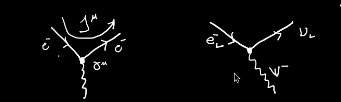
\includegraphics[width=0.75\linewidth]{025.png}
\end{figure}

\begin{tcolorbox}[colback=yellow!10, colframe=blue!20!black, title= Tarea ] 
Mostrar que en el límite ultra relativista. La helicidad es equivalente a la cliralidad.
 
\end{tcolorbox}

\begin{tcolorbox}[colback=yellow!10, colframe=red!20!black, title= Tarea ] 

Mostrar que la ecuación de Dirac es covariante Lorentz. 

\[
i \gamma^\mu \frac{\partial \psi }{\partial x^\mu  }- m \psi =0
\]
 
\end{tcolorbox}


\subsection{13 de mayo}


Tenemos la interacción: 
\[
e^{-}e^{-} \to e^{-} e^{-}
\]
%\includegraphics[]{diagrama13}


\begin{align*}
    T_{fi}^{(1)} &= -i \int d^2 \mathcal{X}  \dot{\mathcal{J}}_\mu \hspace{5ex} 
         \mathcal{J}^\mu = \overline{\psi} \gamma ^\mu \psi  \quad \psi = \mathcal{U }(p) e^{-px} \\
 T_{fi}^{(1)} &= (-e \overline{ \mathcal{U}_c  } \gamma^\mu  \mathcal{U}_A   )\qty( -\frac{\eta_{\mu \nu }}{q^2})(\overline{ -\mathcal{U}  }_D \gamma^\mu  \mathcal{U}_B)   \int d^2 \mathcal{X}         e^{i p_C\cdot \mathcal{X}-p_A\cdot \mathcal{X} +p_D\cdot \mathcal{X}-p_B\cdot \mathcal{X}} 
\end{align*}









Si haceamos el otro diagrama: 
%\includegraphics[]{diagrama132}


\[
\mathcal{M} = \mathcal{M}_a+\mathcal{M}_b 
\]
Necesito que mi función sea anti simetríca, dbemos incluir el signo menos.  

\begin{align*}
    -i \mathcal{M}_b = -\qty(i e \overline{\mathcal{U} }_D \gamma^\mu \mathcal{U}_A ) \qty(-\frac{\eta_{ \mu \nu }}{q^2 } ) (i e \overline{\mathcal{U}}_C \gamma^\nu  \mathcal{U}_B )
\end{align*}
Cuando sumo los espinores, debo de considerar todos los espinores. 


En la sección eficaz usamos: 

\[
\abs{\mathcal{M}}^2 \to \overline{\abs{\mathcal{M}}^2 } = \frac{1}{2S_A+1  } \frac{1}{ 2S_B+1} \sum_{Spin} \abs{\mathcal{M}}^2
\]

$\mathcal{M}(\uparrow_A \uparrow_B\to \uparrow_C \uparrow_D) = \mathcal{M} = (\downarrow_A \downarrow _B \to  \downarrow _C \downarrow_D) =  e ^2\frac{(2m) (2m) }{(P_D-P_A)^2 }   - \frac{e^2 (2m)^2 }{(P_C -P_A)^2  }  = -e^2 (4m^2)\qty(\frac{1}{t} - \frac{1}{u} )$

\[
\mathcal{M} (\uparrow \downarrow \to \uparrow \downarrow ) = \mathcal{M} (\downarrow \uparrow \to \downarrow \uparrow  )=0 - \frac{e ^2 (2m)^2 }{(P_C-P_A)^2 }
\]
\[
\mathcal{M} (\uparrow \downarrow \to \downarrow \uparrow )=  \mathcal{M} (\downarrow \uparrow \to \uparrow \downarrow) = \frac{e^2 (2m)^2 }{(P_D-P_A)^2}+0
\]


Primero formamos un poco de intuición: considerando el caso No-Relaticista: $P \to 0$ 

Electrón entratne $ \mathcal{U}^{(s)} = \sqrt{2m}\begin{pmatrix}
    \mathcal{X}^{(s)} \\0
\end{pmatrix}  $

Electrón saliente: $\overline{\mathcal{U}  }^{(s)}\sqrt{2m} \begin{pmatrix}
    \mathcal{X}^{(s)^+  } &0
\end{pmatrix}  $


Entonces: tenemos: (esto es cierto si tenemos la particula con el mismo espín) 
\[
\overline{\mathcal{U}}^{(s)}  \gamma^\mu \mathcal{U}^{(s)} = \begin{cases}
    \mathcal{U}^\dagger \gamma^0\gamma^0 \mathcal{U}  =2m  \\
    \mathcal{U}^\dagger \gamma^0 \gamma^i \mathcal{U} = \begin{pmatrix}
        \mathcal{X  } ^{(s)} &0  
    \end{pmatrix} \begin{pmatrix}
        0&\sigma^i \\\sigma^i &0
    \end{pmatrix} \begin{pmatrix}
        \mathcal{X}^{(s)}  \\0
    \end{pmatrix} =0\quad i =1,2,3
 \end{cases}
\]





\[
\gamma^0\gamma^i = \begin{pmatrix}
    0 &\sigma^k \\ \sigma^k &0
\end{pmatrix} 
\]

\subsubsection{variables  de interacción de dos a dos} 

\[
A+B \to C+D
\]
puedo construir:
\[
P_A\cdot P_B \quad P_A\cdot P_C\quad P_A\cdot P_D
\]
sabemos que $P_i ^2 =m_i^2$ también que: $P_A+P_B=P_C+P_D$

Escogemos las siguientes variables: 
\begin{align*}
    S &= (P_A+P_B)^2 \\
    t &= (P_A-P_C)^2 \\
    u &= (P_A-P_D)^2
\end{align*}

\[
S+t+u= m_A^2+m_B^2+m_C^2+m_D^2
\]
\subsection*{Normalización}  


nececitamos que: 
\[
\rho = \psi^\dagger \psi
\]
A esto le llamamos normalización covariante, esto es: 
\[
\int \rho d V= \int \psi ^\dagger \psi d V = 2E 
\]
Si tomo un valor mayor que 1, se cumple la ecuación anterior.  al fijar esta normalización. y partiendo del espinor: 

\[
u^{(s)} = N \begin{pmatrix}
    \mathcal{X }^{(s)} \\
    \frac{\sigma \cdot P}{ E+m} \mathcal{X }^{(s)}
\end{pmatrix} \quad u^{(r)^\dagger u^{(s)}  } = 2E \delta_{rs  }
\]

\begin{tcolorbox}[colback=red!10, colframe=red!20!black, title=Ejercicio  ] 
 mostar que 
\begin{align}
    \overline{ u}^{(s) }u ^{(s)} &=2m \\
    \overline{ v}^{(s) }v ^{(s)} &=2m 
\end{align}
Derivar las relaciones de completitud: 
\begin{align*}
    \sum_{s=1,2} u ^{(s)}(P) \overline{ u}^{(s) }(P)  = \not P+ m \mathbb{I} \\
    \sum_{s=1,2} v ^{(s)}(P) \overline{ v}^{(s) }(P)  = \not P- m \mathbb{I} \\
\end{align*}
 
\end{tcolorbox}
\begin{tcolorbox}[colback=blue!10, colframe=blue!20!black, title=Ejercicio opcional  ] 

\begin{align*}
    \Lambda_+ &= \frac{ \not P + m }{2m }   \quad \Lambda = \frac{\not P -m}{2m} \\
    \Lambda_\pm^2 &= \Lambda_\pm  \quad \Lambda_+ + \Lambda_- = \mathbb{I}
\end{align*}
\end{tcolorbox}
 

Tomemos la interacción $ e^- \mathcal{M}^-\to e^- \mathcal{M}^- $



%\includegraphics[]{diragrma1303}

\[
-i\mathcal{M} = (i e \overline{\mathcal{U}}(R' , S' )  \gamma^\mu \mathcal{U}_A (R,S))  \qty(\frac{-i}{q^2}) (i e \overline{\mathcal{U}}_D(p' , r' )  \gamma^\mu \mathcal{U}_B (P,r))
\]


La aplitud es : 
\[
\overline{ \abs{ \mathcal{M}}^2 } = \frac{ e ^4}{ q^4} \lfloor_e ^{\hspace{2ex }\mu \nu  } \lfloor_{\mu \nu }^{ \quad muon}
\]

\[
\lfloor_e ^{\hspace{1ex}\mu \nu  } = \frac{1}{2} \sum_{spin} [(i e \overline{\mathcal{U}}(R' , S' )  \gamma^\mu \mathcal{U}_A (R,S))][(i e \overline{\mathcal{U}}_C(R' , S' )  \gamma^\nu \mathcal{U}_A (R,S)) ]^*
\]
Entonces vamos a usar:

\begin{align*}
    &=[\overline{\mathcal{ U}}(R',S')\gamma^\nu \mathcal{ U} (R,S)    ]^\dagger\\
&=[\mathcal{ U}^\dagger (R',S')\gamma^0\gamma^\nu \mathcal{ U}(R,S) ] ^\dagger \\
&= [\mathcal{ U}^\dagger (R,S)(\gamma^\nu)^\dagger \gamma^0 \mathcal{ U}(R',S') ] ^\dagger\\
&= [\mathcal{ U}^\dagger (R,S)\gamma^0\gamma^\nu\gamma^0 \gamma^0 \mathcal{ U}(R',S') ] ^\dagger \\
&= [\overline{\mathcal{ U}} (R ,S )\gamma^\nu \mathcal{ U}(R',S') ]
\end{align*} Entonces:

\[
\lfloor_e ^{\hspace{1ex}\mu \nu  } = \frac{1}{2} \sum_{spin } \qty[i e u(R',S')\gamma ^\mu u_A(R,s)   ] \qty[-ie \overline{ u}(R,S)\gamma^\nu u (R',S')   ]
\]


\[
\lfloor_e ^{\hspace{1ex}\mu \nu  } = = -\frac{e ^2}{2} \sum_{s,s'} \overline{u}_i (R',S') \gamma_{ij} ^\mu  u (R,S)_j \overline{u}_R (R,S) \gamma_{k,l}^\nu u _l (R',S') 
\]

para poder usar la relacion de completitud voy a cambiar de lugar la expresión anterior
\[
\lfloor_e ^{\hspace{1ex}\mu \nu  } = -\frac{e ^2}{2} \sum_{s,s'} \overline{u}_l (R',S') \gamma_{ij} ^\mu  \overline{u_i} (R,S)_j \gamma_{i,j}^\mu u(R,S)_j u_R (R,S)  \gamma _{kl}^\nu 
\]

Usando la relacion de completitud tenemos: 
\begin{align*}
&=\sum_{1,2} u(p,r)_v  \overline{u} (p',r)_y = ( \not P +m \mathbb{I})_{v y} \\
&= \sum_{ijkl} (R' +m)_{li} \gamma_{ij}^\mu (\not R +m )_{jk} \gamma_{kl}^\nu  \\
& =Tr[(\not R ' +m )\gamma ^\mu (\not R+m )\gamma^\nu   ]
\end{align*}






\end{document}
